\documentclass[11pt, titlepage]{article}

\usepackage[letterpaper, hmargin=1in, bmargin=1in, tmargin=1.3in,
headheight=26pt]{geometry}

\usepackage{graphicx}
\usepackage{booktabs}
\usepackage{longtable}
\usepackage{tabularx}
\usepackage{hyperref}
\usepackage{array}   % Used for table formatting
\newcolumntype{P}[1]{>{\raggedright\let\newline\\\arraybackslash\hspace{0pt}}m{#1}}
\newcolumntype{C}[1]{>{\centering\arraybackslash}m{#1}}
\newcolumntype{N}[1]{>{\centering\arraybackslash}p{#1}}
\usepackage{multirow}
\usepackage[shortcuts]{extdash}
\usepackage[usenames,dvipsnames,table]{xcolor}
\usepackage{amsfonts}
\usepackage{amsmath}
\usepackage{float}
\usepackage{pdflscape}

\usepackage[nottoc,notlof,notlot,numbib]{tocbibind}

\usepackage{natbib}

\usepackage[page]{totalcount}

\usepackage{fancyhdr}
\fancyhf{}
\lhead{System, Integration, and Unit Test Plan \\ \progname{}}
\rhead{Geneva M. Smith \\ Dept. of Computing and Software---McMaster University}
\lfoot{Ver.~\ref{current_version_TestPlan}}
\rfoot{\thepage\ of \thepages}

\renewcommand{\footrule}{\vbox to 0pt
    {\makebox[\textwidth]{\hrulefill}\vss}}

\definecolor{CoolPurple}{RGB}{117, 0, 235}
\definecolor{NatureGreen}{RGB}{8, 104, 11}
\definecolor{SeaBlue}{RGB}{6, 97, 122}
\definecolor{Lilac}{RGB}{178, 131, 206}

\hypersetup{
    bookmarks=true,
    colorlinks=true,
    linktoc=all,
    linkcolor=CoolPurple,
    citecolor=NatureGreen,
    filecolor=WildStrawberry,
    urlcolor=SeaBlue
}

\newcommand{\colourRow}{\rowcolor[gray]{0.9}}
\newcommand{\colourCell}{\cellcolor[gray]{0.9}}

\newcommand{\citepg}[2]{\citeauthor{#1}, \citeyear{#1}, p.~#2}
\newcommand{\citeg}[1]{\citeauthor{#1}, \citeyear{#1}}

\makeatletter
\newcommand\newref[1]{#1\def\@currentlabel{#1}}
\makeatother

%% Comments

\usepackage{color}

\newif\ifcomments\commentstrue

\ifcomments
\newcommand{\authornote}[3]{\textcolor{#1}{[#3 ---#2]}}
\newcommand{\todo}[1]{\textcolor{red}{[TODO: #1]}}
\else
\newcommand{\authornote}[3]{}
\newcommand{\todo}[1]{}
\fi

\newcommand{\wss}[1]{\authornote{blue}{SS}{#1}}
\newcommand{\wgs}[1]{\authornote{teal}{GS}{#1}}
\newcommand{\wjc}[1]{\authornote{purple}{JC}{#1}}

\newcommand{\progname}{EMgine} % PUT YOUR PROGRAM NAME HERE

\newcommand{\conceptVersion}{1.0}
\newcommand{\srsVersion}{1.5.1}
\newcommand{\mgversion}{1.5}
\newcommand{\misversion}{0.1.1}
\newcommand{\codeversion}{0.1}
\newcommand{\mastertestplanVersion}{1.0}
\newcommand{\verifytestplanVersion}{1.0}
\newcommand{\validatetestplanVersion}{1.0}
\newcommand{\manualversion}{?}

\newcommand{\timetype}{\mathbb{T}}
\newcommand{\deltatimetype}{\mathbb{T}_{\Delta}}
\newcommand{\energytype}{\mathbb{J}}
\newcommand{\energychangetype}{\mathbb{J}_{\Delta}}
\newcommand{\stringtype}{\text{String}}
\newcommand{\emotionintensitytype}{\mathbb{I}}
\newcommand{\responsestrength}{\mathbb{I}_{\Delta}}
\newcommand{\emotionstatetype}{\mathbb{ES}}
\newcommand{\emotionstatedecaytype}{\mathbb{ES}_\lambda}
\newcommand{\emotiontype}{\mathbb{E}}
\newcommand{\emotionkindstype}{\mathbb{K}}
\newcommand{\emotionequilibriumtype}{\mathbb{ES_{\rightleftharpoons}}}
\newcommand{\emotiondecaytype}{\mathbb{I_{\lambda}}}
\newcommand{\egotype}{\mathbb{O}}
\newcommand{\egoidentitytype}{\mathbb{ID}}
\newcommand{\goaltype}{\mathbb{G}}
\newcommand{\plantype}{\mathbb{P}}
\newcommand{\padpoint}{P_{\left(P,A,D\right)}}
\newcommand{\goallabeltype}{\mathbb{L}}
\newcommand{\worldtype}{\mathbb{W}}
\newcommand{\worldstatetype}{\mathbb{S}}
\newcommand{\worldstatechangetype}{\mathbb{S}_{\Delta}}
\newcommand{\statedistancetype}{\mathbb{D}}
\newcommand{\statedistancechangetype}{\mathbb{D}_{\Delta}}
\newcommand{\indexsettype}{\mathbb{IS}}
\newcommand{\goalegotype}{\mathbb{GE}}
\newcommand{\socialrelationtype}{{R^{S}}}
\newcommand{\socialattachmenttype}{\mathbb{SA}}
\newcommand{\actiontype}{\mathbb{AC}}
\newcommand{\actortype}{\mathbb{A}}
\newcommand{\attentiontype}{\mathbb{AT}_x}
\newcommand{\probabilitytype}{\left[0,1\right]}
\newcommand{\maxval}{\mathsf{MAX}}
\newcommand{\True}{\mathit{True}}
\newcommand{\False}{\mathit{False}}
\newcommand{\defEq}{\text{ } \mathlarger{\mathlarger\circeq} \text{ }}

\newcommand{\mOtherChange}{\mathit{otherChange}}
\newcommand{\mActor}{\mathit{actor}}
\newcommand{\mDeliberate}{\mathit{deliberate}}
\newcommand{\mImportance}{\mathit{importance}}
\newcommand{\mFear}{\mathtt{Fear}}
\newcommand{\mAnger}{\mathtt{Anger}}
\newcommand{\mSadness}{\mathtt{Sadness}}
\newcommand{\mJoy}{\mathtt{Joy}}
\newcommand{\mInterest}{\mathtt{Interest}}
\newcommand{\mSurprise}{\mathtt{Surprise}}
\newcommand{\mDisgust}{\mathtt{Disgust}}
\newcommand{\mTrust}{\mathtt{Acceptance}}
\newcommand{\mStore}{\mathit{Store}}
\newcommand{\mControl}{\mathit{Control}}
\newcommand{\mGenerate}{\mathit{Generate}}
\newcommand{\mDecay}{\mathit{Decay}}
\newcommand{\mAppraisal}{\mathit{Appraisal}}

\usepackage{xr}
\externaldocument{../../SRS/EMgine_SRS}
\newcommand{\rref}[1]{R\ref{#1}}
\newcommand{\nfref}[1]{NF\ref{#1}}

\externaldocument{../../Design/MG/EMgine_MG}
\newcommand{\mref}[1]{M\ref{#1}}

\externaldocument{../MTP/EMgine_MTP}

% From https://tex.stackexchange.com/questions/101040/how-to-remove-unnecessary
% -space-after-flalign-environment
\newenvironment{nospaceflalign*}
{\setlength{\abovedisplayskip}{0pt}\setlength{\belowdisplayskip}{0pt}%
    \csname flalign*\endcsname}
{\csname endflalign*\endcsname\ignorespacesafterend}
%%%

\usepackage[shortlabels, inline]{enumitem}

\begin{document}

    \newcounter{pages}

    \begin{titlepage}

        \thispagestyle{empty}

        \title{System, Integration, and Unit Test Plan for \progname{}: A
        Computational Model of Emotion for Enhancing Non-Player Character
        Believability in Games}
        \author{Geneva M. Smith}
        \date{Version~\ref{current_version_TestPlan} (April 20, 2023)}

        \maketitle

    \end{titlepage}

    \pagestyle{fancy}

    \vspace*{\fill}
    \noindent\textbf{\Large Revision History}
    \begin{center}
        \begin{tabular}{m{0.18\linewidth}C{0.13\linewidth}m{0.59\linewidth}}
            \toprule {\bf Date} & {\bf Version} & {\bf Notes}\\
            \midrule
            \vspace*{1mm}April 20, 2023 &
            \vspace*{1mm}\newref{0.1}\label{current_version_TestPlan} &
            \vspace*{5mm}
            \begin{itemize}[noitemsep, nosep]
                \item Initial document with the Emotion Intensity Component
                (Emotion Intensity Type [\mref{mIntensity}] and Emotion State
                Type [\mref{mStateType}] Modules) based on SRS Version~1.5.1,
                MG Version~1.5, and MIS Version~0.1.1
            \end{itemize} \\
            \bottomrule
        \end{tabular}
    \end{center}
    \vspace*{\fill}

    \clearpage

    \tableofcontents

    \listoftables

    \listoffigures

    \clearpage

    \section{Symbols, Abbreviations and Acronyms}\label{sec:refs}
For \progname{}'s other symbols, abbreviations, and acronyms, see the:
\begin{itemize}
    \item Software Requirement Specification (SRS) at
    \href{https://github.com/GenevaS/EMgine/blob/main/docs/SRS/EMgine_SRS.pdf}{https://github.com/GenevaS/EMgine/blob/
        \newline main/docs/SRS/EMgine\_SRS.pdf}, and
    \item Module Guide (MG) at
    \href{https://github.com/GenevaS/EMgine/blob/main/docs/Design/MG/EMgine_MG.pdf}{https://github.com/GenevaS/EMgine/blob/main/docs/Design/\newline
        MG/EMgine\_MG.pdf}, and
    \item Module Interface Specification (MIS) at
    \href{https://github.com/GenevaS/EMgine/blob/main/docs/Design/MIS/EMgine_MIS.pdf}{https://github.com/GenevaS/EMgine/blob/main/
        \newline docs/Design/MIS/EMgine\_MIS.pdf}.
\end{itemize}

\begin{center}

    \renewcommand{\arraystretch}{1.2}
    \begin{tabular}{c l}
        \toprule
        \textbf{Abbrv.} & \textbf{Description} \\

        \midrule

        \colourRow ATP & Acceptance Test Plan \\

        CME & Computational Model of Emotion \\

        %CS & Computer Science \\

        %\colourRowHCI & Human-Computer Interaction \\

        \colourRow IDE & Integrated Development Environment \\

        M & Module defined in the MG \\

        \colourRow MG & Module Guide \\

        MIS & Module Interface Specification \\

        \colourRow MTP & Master Test Plan \\

        NF & Nonfunctional Requirement defined in the SRS \\

        \colourRow NPC & Non-Player Character (Video Games) \\

        R & Functional Requirement defined in the SRS \\

        \colourRow SDA & Software Development Artifact \\

        %SE & Software Engineering \\

        SIUTP & System, Integration, and Unit Test Plan \\

        \colourRow SDLC & Software Development Life Cycle \\

        SRS & Software Requirements Specification \\

        \colourRow T & Test\\

        V \& V & Verification and Validation \\

        \colourRow VS & Microsoft Visual Studio \\

        \bottomrule

    \end{tabular}

\end{center}

    \clearpage

    \section{Introduction}
This document describes the System, Integration, and Unit Test Plan (SIUTP) for
\progname{}. Its purpose is to describe the testing efforts to verify the
ability of \progname{}'s implementation to meet its functional and
nonfunctional requirements as described in its Software Requirements
Specification (SRS, Version~\srsVersion) and additional data types and models
as described in its Module Guide (MG, Version~\mgversion) and Module Interface
Specification (MIS, Version~\misversion). This also acts as a basis for
regression testing as \progname{} is developed further. It describes tests for
each requirement and module, traceability between tests and \progname{}'s
requirements, and testing and verification tools.

This test plan does \textit{not} include validation efforts to evaluate
\progname{}'s acceptability for its end-users and stakeholders. That
information is in its Acceptance Test Plan (ATP).

The document's content and organization is loosely based on IEEE Std 829-2008
Clause 9: Level Test Plan (LTP)~\citep{vvDocIEEE}.

\subsection{Summary of \progname{}'s Purpose and Design Goals}
\progname{} is a Computational Model of Emotion (CME) for Non-Player Characters
(NPCs) to enhance their believability, with the goal of improving long-term
player engagement. \progname{} is for \textit{emotion generation}, accepting
user-defined information from a game environment to determines what emotion and
intensity a NPC is ``experiencing''. How the emotion is expressed and what
other effects it could have on game entities is left for game
designers/developers to decide.

\progname{} aims to provide a feasible and easy-to-use method for game
designers/developers to include emotion in their NPCs, they perceive to be
challenging with the current tools and
restrictions~\citep{broekens2016emotional}. \progname{} should be modular and
portable such that game designers/developers can use it in their regular
development environment, and should not require knowledge of affective science,
psychology, and/or emotion theories. Therefore, it is a library of components
to maximize a game designer/developer's control over how and when \progname{}
functions.

\subsection{Scope of Testing Efforts}
The overall goals of \progname{}'s system, integration, and unit testing effort
are:
\begin{enumerate}

    \item Ensure traceability between \progname{}'s verification efforts and
    its SRS, MG, and MIS

    \item Build confidence in the correctness and accuracy of \progname{}'s
    source code

    \item Build confidence in \progname{}'s overall verification efforts

\end{enumerate}

This test plan must be \textit{reviewed} for each new major version of
\progname{}'s SRS, MG, and/or MIS and revised accordingly. This ensures that
these testing efforts remain relevant throughout \progname{}'s development. For
new minor versions of \progname{}'s SRS, MG, and/or MIS, the review can be
limited to only those sections related to SRS, MG, and/or MIS modifications to
help reduce the effort required when testing the next major version.

This test plan must be \textit{executed} in full for each new major version of
\progname{}'s source code. Previous versions do not need to be retested. The
SIUTP can be partially executed for new minor versions of the source code to
help reduce the effort required when testing the next major version.

The SIUTP describes the ``Dynamic Testing Method'' for Implementation
Verification referenced in \progname{}'s Master Test Plan (MTP)
Section~\ref{plan:implementation}.

\subsection{Project Organization}
\progname{}'s development uses the general software development life cycle
processes of requirements analysis, architecture and design definition,
implementation, verification, and validation. Each of these processes outputs at
least one Software Development Artifact (SDA) which serves as a description of
the process's results and becomes an input to subsequent processes
(Figure~\ref{fig:dependencies}). Each SDA has an associated verification and/or
validation plan (Table~\ref{tab:verificationPlanLocation}) to ensure that it
adheres to the \progname{}'s concept.

\vspace*{\fill}
\begin{figure}[!h]
    \centering
    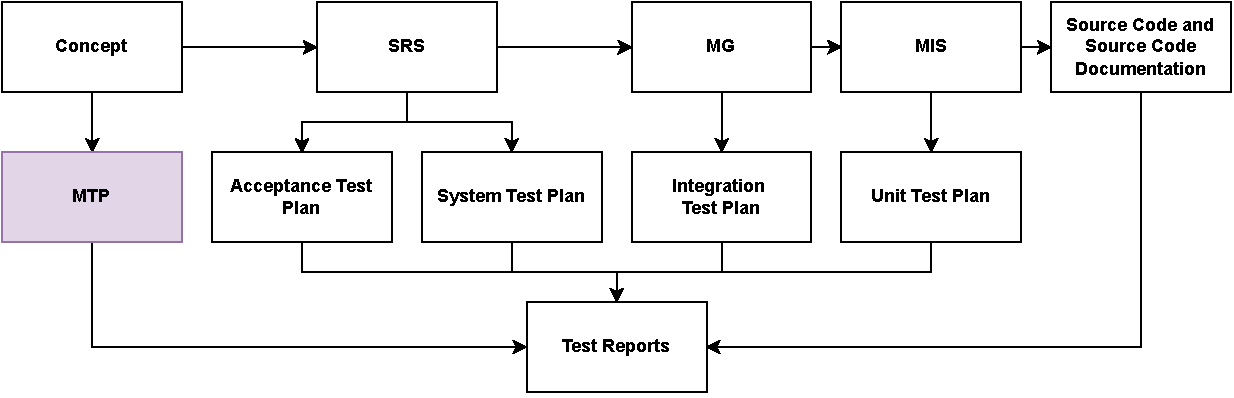
\includegraphics[width=\textwidth]{figures/mtpOrg.pdf}
    \caption{Dependencies Between \progname{}'s SDAs (MTP Highlighted)}
    \label{fig:dependencies}
\end{figure}

\begin{table}[!h]
    \renewcommand{\arraystretch}{1.2}
    \centering
    \caption{Location of V \& V Plans for \progname{}'s SDAs}
    \label{tab:verificationPlanLocation}
    \begin{tabular}{P{0.38\linewidth}P{0.5\linewidth}}
        \toprule
        \textbf{SDA} & \textbf{Location of V \& V Plan} \\

        \midrule

        \colourRow Concept Summary & -- \\

        Master Test Plan & Master Test Plan \\

        \colourRow Software Requirements Specification & Master Test Plan \\

        Module Guide & Master Test Plan \\

        \colourRow Module Interface Specification & Master Test Plan \\

        System, Integration, and Unit Test Plan & Master Test Plan \\

        \colourRow Acceptance Test Plan & Master Test Plan \\

        Source Code and Source Code Documentation& System, Integration, and
        Unit Test Plan \newline Acceptance Test Plan \\

        \bottomrule
    \end{tabular}
\end{table}
\vspace*{\fill}

\subsection{Relevant Documentation}
The Master Test Plan (MTP) refers to the following Software Development
Artifacts (SDAs):
\begin{itemize}

    \item \textbf{Title}: Concept Summary for \progname{}: A Computational
    Model of Emotion for Enhancing Non-Player Character Believability in Games
    \\
    \textbf{Location}:
    \href{https://github.com/GenevaS/EMgine/blob/main/docs/ConceptSummary/EMgine_ConceptSummary.pdf}{https://github.com/GenevaS/EMgine/blob/main/docs/ConceptSummary/\newline
     EMgine\_ConceptSummary.pdf} \\
    \textbf{Description}: Product of the concept definition process. An
    overview of \progname{} purpose, design goals, and motivation.

    \item \textbf{Title}: Software Requirements Specification for \progname{}:
    A Computational Model of Emotion for Enhancing Non-Player Character
    Believability in Games \\
    \textbf{Location}:
    \href{https://github.com/GenevaS/EMgine/blob/main/docs/SRS/EMgine_SRS.pdf}{https://github.com/GenevaS/EMgine/blob/main/docs/SRS/EMgine\_SRS.pdf}
     \\
    \textbf{Description}: Product of the requirements analysis process.
    \progname{}'s problem domain, purpose, underlying models, requirements
    (functional and nonfunctional), and likely changes.

    \item \textbf{Title}: Module Guide for \progname{}: A Computational Model
    of Emotion for Enhancing Non-Player Character Believability in Games \\
    \textbf{Location}:
    \href{https://github.com/GenevaS/EMgine/blob/main/docs/Design/MG/EMgine_MG.pdf}{https://github.com/GenevaS/EMgine/blob/main/docs/Design/MG/\newline
     EMgine\_MG.pdf} \\
    \textbf{Description}: Product of the architecture definition process. An
    overview of \progname{}'s architecture and component modules.

    \item \textbf{Title}: Module Interface Specification for \progname{}: A
    Computational Model of Emotion for Enhancing Non-Player Character
    Believability in Games \\
    \textbf{Location}: TDB \\
    \textbf{Description}: Product of the design definition process.
    Specifications of each module in \progname{} such that they are readily
    implementable.

    \item \textbf{Title}: Source Code and Documentation for \progname{}: A
    Computational Model of Emotion for Enhancing Non-Player Character
    Believability in Games \\
    \textbf{Location}: TDB \\
    \textbf{Description}: Product of the implementation process. A
    software-based realization of \progname{}'s requirements and design,
    accompanied by documentation of the resulting components and/or processes.

    \item \textbf{Title}: User Manual for \progname{}: A Computational Model
    of Emotion for Enhancing Non-Player Character Believability in Games \\
    \textbf{Location}: TDB \\
    \textbf{Description}: Product of the implementation process. A document
    written for \progname{}'s users to help them learn about and use
    \progname{}.

\end{itemize}

\noindent \progname{} has additional test plan documents as follows:
\begin{itemize}

    \item \textbf{Title}: System, Integration, and Unit Test Plan for
    \progname{}: A Computational Model of Emotion for Enhancing Non-Player
    Character Believability in Games \\
    \textbf{Location}: TDB \\
    \textbf{Description}: Test specifications to evaluate \progname{}'s models
    with respect to its design specifications (see
    Section~\ref{plan:implementation}).

    \clearpage\item \textbf{Title}: Acceptance Test Plan for \progname{}: A
    Computational Model of Emotion for Enhancing Non-Player Character
    Believability in Games \\
    \textbf{Location}: TDB \\
    \textbf{Description}: Test specifications to evaluate the ability of
    \progname{}'s models to produce expected emotions and intensities (see
    Section~\ref{plan:validate}).

\end{itemize}

\noindent This document also refers to the:
\begin{itemize}

    \item IEEE Standard for Software and System Test Documentation (IEEE
    Std 829-2008)~\citep{vvDocIEEE} to inform the creation of this document,
    the System, Integration, and Unit Test Plan, and the Acceptance Test Plan

    \item IEEE Standard for System, Software, and Hardware Verification and
    Validation (IEEE Std 1012-2016)~\citep{vvIEEE} to inform the creation of
    this document and the System, Integration, and Unit Test Plan

    \item IEEE Recommended Practice for Software Requirements Specifications
    (IEEE Std 830-1998 (R2009))~\citep{srsIEEE} to inform the evaluation of
    \progname{}'s Software Requirements Specification (SRS)

    \item ISO/IEC/IEEE International Standard - Systems and software
    engineering -- System life cycle processes (ISO/IEC/IEEE
    15288:2015(E))~\citep{slcIEEE} to inform the evaluation of \progname{}'s
    design

\end{itemize}

\subsection{Testing and Verification Tools}\label{sec:tools}
\progname{}'s development uses the C\# programming language because it is one
of the languages supported in Unity, a well-known game development
platform~\citep{unity3Dcsharp}. The supporting Integrated Development
Environment (IDE), Microsoft Visual Studio (VS), is the default script editor
in Unity. \progname{} development uses VS 2022 (Community Edition), which can
access the following tools:
\begin{itemize}

    \item \textbf{NUnit Unit Testing Framework} \\
    This supports the bulk of the automated testing approach for unit,
    integration, system, and regression testing. The IDE is configured to
    automatically run existing unit tests when it is compiling the code base.
    Unity Testing Framework uses custom integration of NUnit
    3.5~\citep{unity3Dtestingfw}.

    \item \textbf{Moq Library for .NET} \\
    This supports tests that rely on components that do not have a concrete
    implementation, such as the user-defined data types
    %(Section~\ref{sec_sysUserDataTypes}).
    It allows the definition of mocked
    interface calls within unit tests that are type-safe~\citep{moq}.

    \item \textbf{Performance Analysis} \\
    \progname{} uses the performance tools built into VS 2022, which includes
    CPU, memory, and time usage tools~\citep{vs2022perf}.

    \item \textbf{Code Style and Quality Analyzers} \\
    \progname{}'s development uses the official .NET Compiler Platform
    (Roslyn)~\citep{roslyn} and the third-party Roslynator~\citep{roslynator}
    analyzers to help adhere to good code quality and style practices. The
    Unity documentation also references Roslyn analyzers for code style and
    quality~\citep{unity3Droslyn}.

\end{itemize}

    \clearpage

    \section{System and Integration Test Description}\label{siutp_SystemTests}
These tests evaluate \progname{}'s implementation for adherence to the solution
described in the Software Requirements Specification (SRS). Dependencies
between data types and methods means that some tests are also integration-level
tests.

\subsection{Tests for Functional Requirements}
\progname{}'s SRS clearly distinguishes between its data types and methods.
Therefore, the test plan separates tests into groups for \progname{}-defined
data types (Section~\ref{sec_sysDataTypes}) and methods
(Section~\ref{sec_sysMethods}).

\subsubsection{\progname{}-Defined Data Types}\label{sec_sysDataTypes}
These tests evaluate the correctness and precision of \progname{}-defined data
types as described in the SRS. Tests that check for adherence to data type
constraints (\rref{R_Types}) also address \progname{}'s response to recoverable
(Section~\ref{sec:sys-nf-recover}) %and non-recoverable
%(Section~\ref{sec:sys-nf-nonrecover})
 errors. Unless otherwise specified:
\begin{itemize}
    \item The NUnit Unit Testing Framework (Section~\ref{sec:tools}) automates
    all tests,
    \item Tests have an error tolerance $\epsilon = 1 \times 10^{-15}$, and
    \item All user messages are printed to the console.
\end{itemize}

\noindent Section~\ref{sec_unitFunctional} describes tests of other functions
necessary to manipulate data types that are \textit{not} described in the SRS.

\paragraph{\thesubsubsection.1 Emotion Intensity $\emotionintensitytype$ and
Intensity Change
$\responsestrength$}\label{sec_IntensityAndIntensityChg}
These tests check the satisfaction of \rref{R_IntensityTypeUse},
\rref{R_IntensityChangeType}, and adherence to the constraints on
$\emotionintensitytype$ and $\responsestrength$ (\rref{R_Types}). This includes
testing their constructors and comparison methods.

\begin{enumerate}

    \item{systemtest-IntensityConstructor\_GivenPositiveNumber}
    \begin{table}[H]
        \centering
        \begin{tabular}{P{0.25\linewidth}P{0.6\linewidth}}
            \toprule
            \textbf{Initial State} & New Session \\
            \textbf{Input} & $5 : \mathbb{R}$ \\ \midrule
            \textbf{Expected Output} & $5 : \emotionintensitytype$ \\
            \textbf{User Message} & -- \\ \bottomrule
        \end{tabular}
    \end{table}

    \item{systemtest-IntensityConstructor\_GivenPositiveNumberWithDecimals-1}
    \begin{table}[H]
        \centering
        \begin{tabular}{P{0.25\linewidth}P{0.6\linewidth}}
            \toprule
            \textbf{Initial State} & New Session \\
            \textbf{Input} & $5.8 : \mathbb{R}$ \\ \midrule
            \textbf{Expected Output} & $5.8 : \emotionintensitytype$ \\
            \textbf{User Message} & -- \\ \bottomrule
        \end{tabular}
    \end{table}

    \clearpage

    \item{systemtest-IntensityConstructor\_GivenPositiveNumberWithDecimals-2}
    \begin{table}[H]
        \centering
        \begin{tabular}{P{0.25\linewidth}P{0.6\linewidth}}
            \toprule
            \textbf{Initial State} & New Session \\
            \textbf{Input} & $2.000000000000001 : \mathbb{R}$ \\ \midrule
            \textbf{Expected Output} & $2.000000000000001 :
            \emotionintensitytype$ \\
            \textbf{User Message} & -- \\ \bottomrule
        \end{tabular}
    \end{table}

    \item{systemtest-IntensityConstructor\_GivenZero}
    \begin{table}[H]
        \centering
        \begin{tabular}{P{0.25\linewidth}P{0.6\linewidth}}
            \toprule
            \textbf{Initial State} & New Session \\
            \textbf{Input} & $0 : \mathbb{R}$ \\ \midrule
            \textbf{Expected Output} & $0 : \emotionintensitytype$ \\
            \textbf{User Message} & -- \\ \bottomrule
        \end{tabular}
    \end{table}

    \item{systemtest-IntensityConstructor\_GivenNegativeNumber}
    \begin{table}[H]
        \centering
        \begin{tabular}{P{0.25\linewidth}P{0.6\linewidth}}
            \toprule
            \textbf{Initial State} & New Session \\
            \textbf{Input} & $-5 : \mathbb{R}$ \\ \midrule
            \textbf{Expected Output} & $0 : \emotionintensitytype$ \\
            \textbf{Test Case Derivation} & When given a negative value,
            \progname{} sets the intensity value to $0$ because values of
            $\emotionintensitytype$ must be $\geq 0$.\\
            \textbf{User Message} & \texttt{Warning: Value for emotion
            intensity is out of bounds. Clamping to the range [0, infty).} \\
            \bottomrule
        \end{tabular}
    \end{table}

    \item{systemtest-IntensityChgConstructor\_GivenPositiveNumber}
    \begin{table}[H]
        \centering
        \begin{tabular}{P{0.25\linewidth}P{0.6\linewidth}}
            \toprule
            \textbf{Initial State} & New Session \\
            \textbf{Input} & $5 : \mathbb{R}$ \\ \midrule
            \textbf{Expected Output} & $5 : \responsestrength$ \\
            \textbf{User Message} & -- \\ \bottomrule
        \end{tabular}
    \end{table}

    \item{systemtest-IntensityChgConstructor\_GivenPositiveNumberWithDecimals-1}
    \begin{table}[H]
        \centering
        \begin{tabular}{P{0.25\linewidth}P{0.6\linewidth}}
            \toprule
            \textbf{Initial State} & New Session \\
            \textbf{Input} & $5.8 : \mathbb{R}$ \\ \midrule
            \textbf{Expected Output} & $5.8 : \responsestrength$ \\
            \textbf{User Message} & -- \\ \bottomrule
        \end{tabular}
    \end{table}

    \clearpage

    \item{systemtest-IntensityChgConstructor\_GivenPositiveNumberWithDecimals-2}
    \begin{table}[H]
        \centering
        \begin{tabular}{P{0.25\linewidth}P{0.6\linewidth}}
            \toprule
            \textbf{Initial State} & New Session \\
            \textbf{Input} & $2.000000000000001 : \mathbb{R}$ \\ \midrule
            \textbf{Expected Output} & $2.000000000000001 : \responsestrength$
            \\
            \textbf{User Message} & -- \\ \bottomrule
        \end{tabular}
    \end{table}

    \item{systemtest-IntensityChgConstructor\_GivenZero}
    \begin{table}[H]
        \centering
        \begin{tabular}{P{0.25\linewidth}P{0.6\linewidth}}
            \toprule
            \textbf{Initial State} & New Session \\
            \textbf{Input} & $0 : \mathbb{R}$ \\ \midrule
            \textbf{Expected Output} & $0 : \responsestrength$ \\
            \textbf{User Message} & -- \\ \bottomrule
        \end{tabular}
    \end{table}

    \item{systemtest-IntensityChgConstructor\_GivenNegativeNumber}
    \begin{table}[H]
        \centering
        \begin{tabular}{P{0.25\linewidth}P{0.6\linewidth}}
            \toprule
            \textbf{Initial State} & New Session \\
            \textbf{Input} & $-5 : \mathbb{R}$ \\ \midrule
            \textbf{Expected Output} & $-5 : \responsestrength$ \\
            \textbf{User Message} & -- \\ \bottomrule
        \end{tabular}
    \end{table}



    \item{systemtest-IntensityChgConstructor\_GivenNegativeNumberWithDecimals}
    \begin{table}[H]
        \centering
        \begin{tabular}{P{0.25\linewidth}P{0.6\linewidth}}
            \toprule
            \textbf{Initial State} & New Session \\
            \textbf{Input} & $-1.000000000000007 : \mathbb{R}$ \\ \midrule
            \textbf{Expected Output} & $-1.000000000000007 : \responsestrength$
            \\
            \textbf{User Message} & -- \\ \bottomrule
        \end{tabular}
    \end{table}

    \item{systemtest-CompareToIntensity\_FirstIsLarger-1}
    \begin{table}[H]
        \centering
        \begin{tabular}{P{0.25\linewidth}P{0.6\linewidth}}
            \toprule
            \textbf{Initial State} & $\mathit{i1} : \emotionintensitytype = 5$,
            $\mathit{i2} : \emotionintensitytype = 1$ \\
            \textbf{Input} & $\mathit{i1}$.CompareToIntensity($\mathit{i2}$) \\
            \midrule
            \textbf{Expected Output} & $1 : \mathbb{Z}$ \\
            \textbf{User Message} & -- \\ \bottomrule
        \end{tabular}
    \end{table}

    \item{systemtest-CompareToIntensity\_FirstIsLarger-2}
    \begin{table}[H]
        \centering
        \begin{tabular}{P{0.25\linewidth}P{0.6\linewidth}}
            \toprule
            \textbf{Initial State} & $\mathit{i1} : \emotionintensitytype = 5$,
            $\mathit{i2} : \emotionintensitytype = 2.1$ \\
            \textbf{Input} & $\mathit{i1}$.CompareToIntensity($\mathit{i2}$) \\
            \midrule
            \textbf{Expected Output} & $1 : \mathbb{Z}$ \\
            \textbf{User Message} & -- \\ \bottomrule
        \end{tabular}
    \end{table}

    \item{systemtest-CompareToIntensity\_FirstIsSmaller-1}
    \begin{table}[H]
        \centering
        \begin{tabular}{P{0.25\linewidth}P{0.6\linewidth}}
            \toprule
            \textbf{Initial State} & $\mathit{i1} : \emotionintensitytype = 1$,
            $\mathit{i2} : \emotionintensitytype = 5$ \\
            \textbf{Input} & $\mathit{i1}$.CompareToIntensity($\mathit{i2}$) \\
            \midrule
            \textbf{Expected Output} & $-1 : \mathbb{Z}$ \\
            \textbf{User Message} & -- \\ \bottomrule
        \end{tabular}
    \end{table}

    \item{systemtest-CompareToIntensity\_FirstIsSmaller-2}
    \begin{table}[H]
        \centering
        \begin{tabular}{P{0.25\linewidth}P{0.6\linewidth}}
            \toprule
            \textbf{Initial State} & $\mathit{i1} : \emotionintensitytype = 5$,
            $\mathit{i2} : \emotionintensitytype = 5.8$ \\
            \textbf{Input} & $\mathit{i1}$.CompareToIntensity($\mathit{i2}$) \\
            \midrule
            \textbf{Expected Output} & $-1 : \mathbb{Z}$ \\
            \textbf{User Message} & -- \\ \bottomrule
        \end{tabular}
    \end{table}

    \item{systemtest-CompareToIntensity\_FirstIsSmaller-3}
    \begin{table}[H]
        \centering
        \begin{tabular}{P{0.25\linewidth}P{0.6\linewidth}}
            \toprule
            \textbf{Initial State} & $\mathit{i1} : \emotionintensitytype = 2$,
            $\mathit{i2} : \emotionintensitytype = 2.000000000000001$ \\
            \textbf{Input} & $\mathit{i1}$.CompareToIntensity($\mathit{i2}$) \\
            \midrule
            \textbf{Expected Output} & $-1 : \mathbb{Z}$ \\
            \textbf{User Message} & -- \\ \bottomrule
        \end{tabular}
    \end{table}

    \item{systemtest-CompareToIntensity\_EqualValues}
    \begin{table}[H]
        \centering
        \begin{tabular}{P{0.25\linewidth}P{0.6\linewidth}}
            \toprule
            \textbf{Initial State} & $\mathit{i1} : \emotionintensitytype = 5$,
            $\mathit{i2} : \emotionintensitytype = 5$ \\
            \textbf{Input} & $\mathit{i1}$.CompareToIntensity($\mathit{i2}$) \\
            \midrule
            \textbf{Expected Output} & $0 : \mathbb{Z}$ \\
            \textbf{User Message} & -- \\ \bottomrule
        \end{tabular}
    \end{table}

    \item{systemtest-EqualsMinIntensity\_IntensityIsLarger-1}
    \begin{table}[H]
        \centering
        \begin{tabular}{P{0.25\linewidth}P{0.6\linewidth}}
            \toprule
            \textbf{Initial State} & $\mathit{i} : \emotionintensitytype = 5$,
            $\mathit{i_{min}} : \emotionintensitytype = 0$ \\
            \textbf{Input} & $\mathit{i}$.EqualsMinIntensity() \\ \midrule
            \textbf{Expected Output} & $\False : \mathbb{B}$ \\
            \textbf{User Message} & -- \\ \bottomrule
        \end{tabular}
    \end{table}



    \item{systemtest-EqualsMinIntensity\_IntensityIsLarger-2}
    \begin{table}[H]
        \centering
        \begin{tabular}{P{0.25\linewidth}P{0.6\linewidth}}
            \toprule
            \textbf{Initial State} & $\mathit{i} : \emotionintensitytype$ =
            2.3, $\mathit{i_{min}} : \emotionintensitytype = 0$ \\
            \textbf{Input} & $\mathit{i}$.EqualsMinIntensity() \\ \midrule
            \textbf{Expected Output} & $\False : \mathbb{B}$ \\
            \textbf{User Message} & -- \\ \bottomrule
        \end{tabular}
    \end{table}

    \item{systemtest-EqualsMinIntensity\_IntensityIsLarger-3}
    \begin{table}[H]
        \centering
        \begin{tabular}{P{0.25\linewidth}P{0.6\linewidth}}
            \toprule
            \textbf{Initial State} & $\mathit{i} : \emotionintensitytype =
            0.000000000000001$, $\mathit{i_{min}} : \emotionintensitytype = 0$
            \\
            \textbf{Input} & $\mathit{i}$.EqualsMinIntensity() \\
            \midrule
            \textbf{Expected Output} & $\False : \mathbb{B}$ \\
            \textbf{User Message} & -- \\ \bottomrule
        \end{tabular}
    \end{table}

    \item{systemtest-EqualsMinIntensity\_IntensityIsMin}
    \begin{table}[H]
        \centering
        \begin{tabular}{P{0.25\linewidth}P{0.6\linewidth}}
            \toprule
            \textbf{Initial State} & $\mathit{i} : \emotionintensitytype = 0$,
            $\mathit{i_{min}} : \emotionintensitytype = 0$ \\
            \textbf{Input} & $\mathit{i}$.EqualsMinIntensity() \\
            \midrule
            \textbf{Expected Output} & $\True : \mathbb{B}$ \\
            \textbf{User Message} & -- \\ \bottomrule
        \end{tabular}
    \end{table}

    \item{systemtest-CompareToIntensityChg\_FirstIsLarger-1}
    \begin{table}[H]
        \centering
        \begin{tabular}{P{0.25\linewidth}P{0.6\linewidth}}
            \toprule
            \textbf{Initial State} & $\mathit{d1} : \responsestrength = 5$,
            $\mathit{d2} : \responsestrength = 0$ \\
            \textbf{Input} & $\mathit{d1}$.CompareToIntensityChg($\mathit{d2}$)
            \\ \midrule
            \textbf{Expected Output} & $1 : \mathbb{Z}$ \\
            \textbf{User Message} & -- \\ \bottomrule
        \end{tabular}
    \end{table}

    \item{systemtest-CompareToIntensityChg\_FirstIsLarger-2}
    \begin{table}[H]
        \centering
        \begin{tabular}{P{0.25\linewidth}P{0.6\linewidth}}
            \toprule
            \textbf{Initial State} & $\mathit{d1} : \responsestrength = 5.8$,
            $\mathit{d2} : \responsestrength = 2.1$ \\
            \textbf{Input} & $\mathit{d1}$.CompareToIntensityChg($\mathit{d2}$)
            \\ \midrule
            \textbf{Expected Output} & $1 : \mathbb{Z}$ \\
            \textbf{User Message} & -- \\ \bottomrule
        \end{tabular}
    \end{table}

    \item{systemtest-CompareToIntensityChg\_FirstIsLarger-3}
    \begin{table}[H]
        \centering
        \begin{tabular}{P{0.25\linewidth}P{0.6\linewidth}}
            \toprule
            \textbf{Initial State} & $\mathit{d1} : \responsestrength = 5.8$,
            $\mathit{d2} : \responsestrength = -1.7$ \\
            \textbf{Input} & $\mathit{d1}$.CompareToIntensityChg($\mathit{d2}$)
            \\ \midrule
            \textbf{Expected Output} & $1 : \mathbb{Z}$ \\
            \textbf{User Message} & -- \\ \bottomrule
        \end{tabular}
    \end{table}

    \item{systemtest-CompareToIntensityChg\_FirstIsSmaller-1}
    \begin{table}[H]
        \centering
        \begin{tabular}{P{0.25\linewidth}P{0.6\linewidth}}
            \toprule
            \textbf{Initial State} & $\mathit{d1} : \responsestrength = 0$,
            $\mathit{d2} : \responsestrength = 5$ \\
            \textbf{Input} & $\mathit{d1}$.CompareToIntensityChg($\mathit{d2}$)
            \\ \midrule
            \textbf{Expected Output} & $-1 : \mathbb{Z}$ \\
            \textbf{User Message} & -- \\ \bottomrule
        \end{tabular}
    \end{table}

    \item{systemtest-CompareToIntensityChg\_FirstIsSmaller-2}
    \begin{table}[H]
        \centering
        \begin{tabular}{P{0.25\linewidth}P{0.6\linewidth}}
            \toprule
            \textbf{Initial State} & $\mathit{d1} : \responsestrength = 5$,
            $\mathit{d2} : \responsestrength = 5.8$ \\
            \textbf{Input} & $\mathit{d1}$.CompareToIntensityChg($\mathit{d2}$)
            \\ \midrule
            \textbf{Expected Output} & $-1 : \mathbb{Z}$ \\
            \textbf{User Message} & -- \\ \bottomrule
        \end{tabular}
    \end{table}

    \item{systemtest-CompareToIntensityChg\_FirstIsSmaller-3}
    \begin{table}[H]
        \centering
        \begin{tabular}{P{0.25\linewidth}P{0.6\linewidth}}
            \toprule
            \textbf{Initial State} & $\mathit{d1} : \responsestrength = -1.7$,
            $\mathit{d2} : \responsestrength = 5.8$ \\
            \textbf{Input} & $\mathit{d1}$.CompareToIntensityChg($\mathit{d2}$)
            \\ \midrule
            \textbf{Expected Output} & $-1 : \mathbb{Z}$ \\
            \textbf{User Message} & -- \\ \bottomrule
        \end{tabular}
    \end{table}

    \item{systemtest-CompareToIntensityChg\_FirstIsSmaller-4}
    \begin{table}[H]
        \centering
        \begin{tabular}{P{0.25\linewidth}P{0.6\linewidth}}
            \toprule
            \textbf{Initial State} & $\mathit{d1} : \responsestrength = -1.7$,
            $\mathit{d2} : \responsestrength = 0$ \\
            \textbf{Input} & $\mathit{d1}$.CompareToIntensityChg($\mathit{d2}$)
            \\ \midrule
            \textbf{Expected Output} & $-1 : \mathbb{Z}$ \\
            \textbf{User Message} & -- \\ \bottomrule
        \end{tabular}
    \end{table}

    \item{systemtest-CompareToIntensityChg\_FirstIsSmaller-5}
    \begin{table}[H]
        \centering
        \begin{tabular}{P{0.25\linewidth}P{0.6\linewidth}}
            \toprule
            \textbf{Initial State} & $\mathit{d1} : \responsestrength = 5$,
            $\mathit{d2} : \responsestrength = 5.000000000000001$ \\
            \textbf{Input} & $\mathit{d1}$.CompareToIntensityChg($\mathit{d2}$)
            \\ \midrule
            \textbf{Expected Output} & $-1 : \mathbb{Z}$ \\
            \textbf{User Message} & -- \\ \bottomrule
        \end{tabular}
    \end{table}

    \item{systemtest-CompareIntensityChg\_EqualValues}
    \begin{table}[H]
        \centering
        \begin{tabular}{P{0.25\linewidth}P{0.6\linewidth}}
            \toprule
            \textbf{Initial State} & $\mathit{d1} : \responsestrength = 5$,
            $\mathit{d2} : \responsestrength = 5$ \\
            \textbf{Input} & $\mathit{d1}$.CompareToIntensityChg($\mathit{d2}$)
            \\ \midrule
            \textbf{Expected Output} & $0 : \mathbb{Z}$ \\
            \textbf{User Message} & -- \\ \bottomrule
        \end{tabular}
    \end{table}


    \item{systemtest-CompareIntensityChgtoMinIntensity\_ChgIsLarger-1}
    \begin{table}[H]
        \centering
        \begin{tabular}{P{0.25\linewidth}P{0.6\linewidth}}
            \toprule
            \textbf{Initial State} & $\mathit{d} : \responsestrength = 5$,
            $\mathit{i_{min}} : \emotionintensitytype = 0$ \\
            \textbf{Input} & $\mathit{d}$.CompareToMinIntensity() \\ \midrule
            \textbf{Expected Output} & $1 : \mathbb{Z}$ \\
            \textbf{User Message} & -- \\ \bottomrule
        \end{tabular}
    \end{table}

    \item{systemtest-CompareIntensityChgtoMinIntensity\_ChgIsLarger-2}
    \begin{table}[H]
        \centering
        \begin{tabular}{P{0.25\linewidth}P{0.6\linewidth}}
            \toprule
            \textbf{Initial State} & $\mathit{d} : \responsestrength = 5.8$,
            $\mathit{i_{min}} : \emotionintensitytype = 0$ \\
            \textbf{Input} & $\mathit{d}$.CompareToMinIntensity() \\ \midrule
            \textbf{Expected Output} & $1 : \mathbb{Z}$ \\
            \textbf{User Message} & -- \\ \bottomrule
        \end{tabular}
    \end{table}

    \item{systemtest-CompareIntensityChgtoMinIntensity\_ChgIsLarger-3}
    \begin{table}[H]
        \centering
        \begin{tabular}{P{0.25\linewidth}P{0.6\linewidth}}
            \toprule
            \textbf{Initial State} & $\mathit{d} : \responsestrength = 2.1$,
            $\mathit{i_{min}} : \emotionintensitytype = 0$ \\
            \textbf{Input} & $\mathit{d}$.CompareToMinIntensity() \\ \midrule
            \textbf{Expected Output} & $1 : \mathbb{Z}$ \\
            \textbf{User Message} & -- \\ \bottomrule
        \end{tabular}
    \end{table}

    \item{systemtest-CompareIntensityChgtoMinIntensity\_ChgIsSmaller-1}
    \begin{table}[H]
        \centering
        \begin{tabular}{P{0.25\linewidth}P{0.6\linewidth}}
            \toprule
            \textbf{Initial State} & $\mathit{d} : \responsestrength = -5$,
            $\mathit{i_{min}} : \emotionintensitytype = 0$ \\
            \textbf{Input} & $\mathit{d}$.CompareToMinIntensity() \\ \midrule
            \textbf{Expected Output} & $-1 : \mathbb{Z}$ \\
            \textbf{User Message} & -- \\ \bottomrule
        \end{tabular}
    \end{table}

    \item{systemtest-CompareIntensityChgtoMinIntensity\_ChgIsSmaller-2}
    \begin{table}[H]
        \centering
        \begin{tabular}{P{0.25\linewidth}P{0.6\linewidth}}
            \toprule
            \textbf{Initial State} & $\mathit{d} : \responsestrength = -1.7$,
            $\mathit{i_{min}} : \emotionintensitytype = 0$ \\
            \textbf{Input} & $\mathit{d}$.CompareToMinIntensity() \\ \midrule
            \textbf{Expected Output} & $-1 : \mathbb{Z}$ \\
            \textbf{User Message} & -- \\ \bottomrule
        \end{tabular}
    \end{table}

    \item{systemtest-CompareIntensityChgtoMinIntensity\_ChgIsSmaller-3}
    \begin{table}[H]
        \centering
        \begin{tabular}{P{0.25\linewidth}P{0.6\linewidth}}
            \toprule
            \textbf{Initial State} & $\mathit{d} : \responsestrength =
            -0.000000000000001$, $\mathit{i_{min}} : \emotionintensitytype = 0$
            \\
            \textbf{Input} & $\mathit{d}$.CompareToMinIntensity() \\ \midrule
            \textbf{Expected Output} & $-1 : \mathbb{Z}$ \\
            \textbf{User Message} & -- \\ \bottomrule
        \end{tabular}
    \end{table}

    \item{systemtest-CompareIntensityChgtoMinIntensity\_ChgIsEqual}
    \begin{table}[H]
        \centering
        \begin{tabular}{P{0.25\linewidth}P{0.6\linewidth}}
            \toprule
            \textbf{Initial State} & $\mathit{d} : \responsestrength = 0$,
            $\mathit{i_{min}} : \emotionintensitytype = 0$ \\
            \textbf{Input} & $\mathit{d}$.CompareToMinIntensity() \\ \midrule
            \textbf{Expected Output} & $0 : \mathbb{Z}$ \\
            \textbf{User Message} & -- \\ \bottomrule
        \end{tabular}
    \end{table}

\end{enumerate}

%\clearpage\paragraph{Emotion Decay Rate $\emotiondecaytype$} These tests check
%the satisfaction of \rref{R_IntensityDecayType} and adherence to the
%constraints on $\emotiondecaytype$ (\rref{R_Types}). This only includes testing
%its constructor.
%
%\begin{enumerate}
%
%    \item{systemtest-DecayRateConstructor1}
%    \begin{table}[H]
%        \centering
%        \begin{tabular}{P{0.25\linewidth}P{0.6\linewidth}}
%            \toprule
%            \textbf{Initial State} & New Session \\
%            \textbf{Input} & $5 : \mathbb{R}$ \\ \midrule
%            \textbf{Expected Output} & $ 5 : \emotiondecaytype$ \\
%            \textbf{User Message} & -- \\ \bottomrule
%        \end{tabular}
%    \end{table}
%
%    \item{systemtest-DecayRateConstructor2}
%    \begin{table}[H]
%        \centering
%        \begin{tabular}{P{0.25\linewidth}P{0.6\linewidth}}
%            \toprule
%            \textbf{Initial State} & New Session \\
%            \textbf{Input} & $2.000000000000001 : \mathbb{R}$ \\ \midrule
%            \textbf{Expected Output} & $ 2.000000000000001 : \emotiondecaytype$
%            \\
%            \textbf{User Message} & -- \\ \bottomrule
%        \end{tabular}
%    \end{table}
%
%    \item{systemtest-DecayRateConstructor3}
%    \begin{table}[H]
%        \centering
%        \begin{tabular}{P{0.25\linewidth}P{0.6\linewidth}}
%            \toprule
%            \textbf{Initial State} & New Session \\
%            \textbf{Input} & $0.000000000000001 : \mathbb{R}$ \\ \midrule
%            \textbf{Expected Output} & $ 0.000000000000001 : \emotiondecaytype$
%            \\
%            \textbf{User Message} & -- \\ \bottomrule
%        \end{tabular}
%    \end{table}
%
%    \item{systemtest-DecayRateConstructorZeroInput}
%    \begin{table}[H]
%        \centering
%        \begin{tabular}{P{0.25\linewidth}P{0.6\linewidth}}
%            \toprule
%            \textbf{Initial State} & New Session \\
%            \textbf{Input} & $0 : \mathbb{R}$ \\ \midrule
%            \textbf{Expected Output} & EM\_DECAY\_RATE\_DEFAULT $ :
%            \emotiondecaytype$ \\
%            \textbf{Test Case Derivation} & When given a negative value,
%            \progname{} sets the decay rate to the default rate because values
%            of $\emotiondecaytype$ must be $> 0$.\\
%            \textbf{User Message} & \texttt{Warning: Emotion cannot decay at a
%                rate of zero or less. Setting to default decay rate of
%                EM\_DECAY\_RATE\_DEFAULT.} \\ \bottomrule
%        \end{tabular}
%    \end{table}
%
%    \clearpage
%
%    \item{systemtest-DecayRateConstructorNegativeInput}
%    \begin{table}[H]
%        \centering
%        \begin{tabular}{P{0.25\linewidth}P{0.6\linewidth}}
%            \toprule
%            \textbf{Initial State} & New Session \\
%            \textbf{Input} & $-5 : \mathbb{R}$ \\ \midrule
%            \textbf{Expected Output} & EM\_DECAY\_RATE\_DEFAULT $ :
%            \emotiondecaytype$ \\
%            \textbf{Test Case Derivation} & When given a negative value,
%            \progname{} sets the decay rate to the default rate because values
%            of $\emotiondecaytype$ must be $> 0$.\\
%            \textbf{User Message} & \texttt{Warning: Emotion cannot decay at a
%                rate of zero or less. Setting to default decay rate of
%                EM\_DECAY\_RATE\_DEFAULT.} \\ \bottomrule
%        \end{tabular}
%    \end{table}
%
%\end{enumerate}
%
%\clearpage\paragraph{Emotion Kinds $\emotionkindstype$} These tests check the
%satisfaction of \rref{R_EmotionKindsType} and adherence to the constraints on
%$\emotionkindstype$ (\rref{R_Types}). This means testing for the presence of
%the expected type, count, and order of emotion kinds.
%
%\begin{enumerate}
%
%    \item{systemtest-JoyKind}
%    \begin{table}[H]
%        \centering
%        \begin{tabular}{P{0.25\linewidth}P{0.6\linewidth}}
%            \toprule
%            \textbf{Initial State} & New Session \\
%            \textbf{Input} & $\emotionkindstype[0] = \mathtt{Joy}$ \\ \midrule
%            \textbf{Expected Output} & $ \True : \mathbb{B}$ \\
%            \textbf{User Message} & -- \\ \bottomrule
%        \end{tabular}
%    \end{table}
%
%    \item{systemtest-SadnessKind}
%    \begin{table}[H]
%        \centering
%        \begin{tabular}{P{0.25\linewidth}P{0.6\linewidth}}
%            \toprule
%            \textbf{Initial State} & New Session \\
%            \textbf{Input} & $\emotionkindstype[1] = \mathtt{Sadness}$ \\
%            \midrule
%            \textbf{Expected Output} & $ \True : \mathbb{B}$ \\
%            \textbf{User Message} & -- \\ \bottomrule
%        \end{tabular}
%    \end{table}
%
%    \item{systemtest-AngerKind}
%    \begin{table}[H]
%        \centering
%        \begin{tabular}{P{0.25\linewidth}P{0.6\linewidth}}
%            \toprule
%            \textbf{Initial State} & New Session \\
%            \textbf{Input} & $\emotionkindstype[2] = \mathtt{Anger}$ \\
%\midrule
%            \textbf{Expected Output} & $ \True : \mathbb{B}$ \\
%            \textbf{User Message} & -- \\ \bottomrule
%        \end{tabular}
%    \end{table}
%
%    \item{systemtest-FearKind}
%    \begin{table}[H]
%        \centering
%        \begin{tabular}{P{0.25\linewidth}P{0.6\linewidth}}
%            \toprule
%            \textbf{Initial State} & New Session \\
%            \textbf{Input} & $\emotionkindstype[3] = \mathtt{Fear}$ \\ \midrule
%            \textbf{Expected Output} & $ \True : \mathbb{B}$ \\
%            \textbf{User Message} & -- \\ \bottomrule
%        \end{tabular}
%    \end{table}
%
%    \item{systemtest-DisgustKind}
%    \begin{table}[H]
%        \centering
%        \begin{tabular}{P{0.25\linewidth}P{0.6\linewidth}}
%            \toprule
%            \textbf{Initial State} & New Session \\
%            \textbf{Input} & $\emotionkindstype[4] = \mathtt{Disgust}$ \\
%            \midrule
%            \textbf{Expected Output} & $ \True : \mathbb{B}$ \\
%            \textbf{User Message} & -- \\ \bottomrule
%        \end{tabular}
%    \end{table}
%
%    \clearpage
%
%    \item{systemtest-AcceptanceKind}
%    \begin{table}[H]
%        \centering
%        \begin{tabular}{P{0.25\linewidth}P{0.6\linewidth}}
%            \toprule
%            \textbf{Initial State} & New Session \\
%            \textbf{Input} & $\emotionkindstype[5] = \mathtt{Acceptance}$ \\
%            \midrule
%            \textbf{Expected Output} & $ \True : \mathbb{B}$ \\
%            \textbf{User Message} & -- \\ \bottomrule
%        \end{tabular}
%    \end{table}
%
%    \item{systemtest-SurpriseKind}
%    \begin{table}[H]
%        \centering
%        \begin{tabular}{P{0.25\linewidth}P{0.6\linewidth}}
%            \toprule
%            \textbf{Initial State} & New Session \\
%            \textbf{Input} & $\emotionkindstype[6] = \mathtt{Surprise}$ \\
%            \midrule
%            \textbf{Expected Output} & $ \True : \mathbb{B}$ \\
%            \textbf{User Message} & -- \\ \bottomrule
%        \end{tabular}
%    \end{table}
%
%    \item{systemtest-InterestKind}
%    \begin{table}[H]
%        \centering
%        \begin{tabular}{P{0.25\linewidth}P{0.6\linewidth}}
%            \toprule
%            \textbf{Initial State} & New Session \\
%            \textbf{Input} & $\emotionkindstype[7] = \mathtt{Interest}$ \\
%            \midrule
%            \textbf{Expected Output} & $ \True : \mathbb{B}$ \\
%            \textbf{User Message} & -- \\ \bottomrule
%        \end{tabular}
%    \end{table}
%
%    \item{systemtest-KindCount}
%    \begin{table}[H]
%        \centering
%        \begin{tabular}{P{0.25\linewidth}P{0.6\linewidth}}
%            \toprule
%            \textbf{Initial State} & New Session \\
%            \textbf{Input} & $| \emotionkindstype | = 8 $ \\ \midrule
%            \textbf{Expected Output} & $ \True : \mathbb{B}$ \\
%            \textbf{Test Case Derivation} & An additional test to ensure there
%            are no more than the eight expected emotion kinds. \\
%            \textbf{User Message} & -- \\ \bottomrule
%        \end{tabular}
%    \end{table}
%
%\end{enumerate}
%
%\clearpage\paragraph{Emotion State
%$\emotionstatetype$}\label{sec:sys-datatypes-emotionstate} These tests check
%the
%satisfaction of \rref{R_EmotionStateType} and adherence to the constraints on
%$\emotionstatetype$ (\rref{R_Types}). This only includes testing its
%constructor.
%
%\begin{enumerate}
%
%    \item{systemtest-EmotionStateConstructor}
%    \begin{table}[H]
%        \centering
%        \begin{tabular}{P{0.25\linewidth}P{0.6\linewidth}}
%            \toprule
%            \textbf{Initial State} & New Session \\
%            \textbf{Input} & $i = \langle \, 2 : \emotionintensitytype, 3.8 :
%            \emotionintensitytype, 40.89 : \emotionintensitytype, 67.3 :
%            \emotionintensitytype, 89.3 : \emotionintensitytype, 34.678 :
%            \emotionintensitytype,$ $ 4.678 : \emotionintensitytype, 78.4 :
%            \emotionintensitytype \, \rangle$, \newline $m = \langle \, 16 :
%            \emotionintensitytype, 10 : \emotionintensitytype, 100 :
%            \emotionintensitytype, 100.536 : \emotionintensitytype, 140.2 :
%            \emotionintensitytype,$ $ 50.7: \emotionintensitytype, 40.78 :
%            \emotionintensitytype, 80.234 : \emotionintensitytype \, \rangle$
%            \\ \midrule
%            \textbf{Expected Output} & $ \{ \mathit{intensities} = i,
%            \mathit{max} = m \} : \emotionstatetype $ \\
%            \textbf{User Message} & -- \\ \bottomrule
%        \end{tabular}
%    \end{table}
%
%    \item{systemtest-EmotionStateConstructorFirstIValueExceedsMValue}
%    \begin{table}[H]
%        \centering
%        \begin{tabular}{P{0.25\linewidth}P{0.6\linewidth}}
%            \toprule
%            \textbf{Initial State} & New Session \\
%            \textbf{Input} & $i = \langle \, 16.1 : \emotionintensitytype, 3.8
%:
%            \emotionintensitytype, 40.89 : \emotionintensitytype, 67.3 :
%            \emotionintensitytype, 89.3 : \emotionintensitytype, 34.678 :
%            \emotionintensitytype,$ $ 4.678 : \emotionintensitytype, 78.4 :
%            \emotionintensitytype \, \rangle$, \newline $m = \langle \, 16 :
%            \emotionintensitytype, 10 : \emotionintensitytype, 100 :
%            \emotionintensitytype, 100.536 : \emotionintensitytype, 140.2 :
%            \emotionintensitytype,$ $ 50.7: \emotionintensitytype, 40.78 :
%            \emotionintensitytype, 80.234 : \emotionintensitytype \, \rangle$
%            \\ \midrule
%            \textbf{Expected Output} & $ \{ \mathit{intensities} = i',
%            \mathit{max} = m \} : \emotionstatetype $, \newline where $i' = i$
%            with $i[0] = m[0]$ \\
%            \textbf{Test Case Derivation} & If $i.k > m.k$, \progname{} sets
%            $\mathit{intensities}.k$ to $m.k$ so that the invariant
%            $\mathit{intensities}.k < \mathit{max}.k$ holds. \\
%            \textbf{User Message} & \texttt{Warning: Value for
%            $\emotionkindstype[0]$ intensity is out of bounds. Clamping to the
%            range [$i[0].$MIN\_INTENTISTY, $m[0]$].} \\ \bottomrule
%        \end{tabular}
%    \end{table}
%
%    \clearpage
%
%    \item{systemtest-EmotionStateConstructorMultiIValueExceedsMValue}
%    \begin{table}[H]
%        \centering
%        \begin{tabular}{P{0.25\linewidth}P{0.6\linewidth}}
%            \toprule
%            \textbf{Initial State} & New Session \\
%            \textbf{Input} & $i = \langle \, 2 : \emotionintensitytype, 3.8 :
%            \emotionintensitytype, 101 : \emotionintensitytype, 67.3 :
%            \emotionintensitytype, 89.3 : \emotionintensitytype, 34.678 :
%            \emotionintensitytype,$ $ 4.678 : \emotionintensitytype, 80.235 :
%            \emotionintensitytype \, \rangle$, \newline $m = \langle \, 16 :
%            \emotionintensitytype, 10 : \emotionintensitytype, 100 :
%            \emotionintensitytype, 100.536 : \emotionintensitytype, 140.2 :
%            \emotionintensitytype,50.7: \emotionintensitytype,$ $  40.78 :
%            \emotionintensitytype, 80.234 : \emotionintensitytype \, \rangle$
%            \\ \midrule
%            \textbf{Expected Output} & $ \{ \mathit{intensities} = i',
%            \mathit{max} = m \} : \emotionstatetype $, \newline where $i' = i$
%            with $i[2] = m[2]$ \\
%            \textbf{Test Case Derivation} & If $i.k > m.k$, \progname{} sets
%            $\mathit{intensities}.k$ to $m.k$ so that the invariant
%            $\mathit{intensities}.k < \mathit{max}.k$ holds. \\
%            \textbf{User Message} & \texttt{Warning: Value for
%            $\emotionkindstype[2]$ intensity is out of bounds. Clamping to the
%            range [$i[2].$MIN\_INTENTISTY, $m[2]$].} \newline
%           \texttt{Warning: Value for $\emotionkindstype[7]$ intensity is out
%           of bounds. Clamping to the range [$i[7].$MIN\_INTENTISTY, $m[7]$].}
%           \\ \bottomrule
%        \end{tabular}
%    \end{table}
%
%    \item{systemtest-EmotionStateConstructorTooFewIntensitiesinI}
%    \begin{table}[H]
%        \centering
%        \begin{tabular}{P{0.25\linewidth}P{0.6\linewidth}}
%            \toprule
%            \textbf{Initial State} & New Session \\
%            \textbf{Input} & $i = \langle \, 2 : \emotionintensitytype, 3.8 :
%            \emotionintensitytype, 40.89 : \emotionintensitytype, 67.3 :
%            \emotionintensitytype, 89.3 : \emotionintensitytype, 34.678 :
%            \emotionintensitytype,$ $ 78.4 : \emotionintensitytype \, \rangle$,
%            \newline $m = \langle \, 16 : \emotionintensitytype, 10 :
%            \emotionintensitytype, 100 : \emotionintensitytype, 100.536 :
%            \emotionintensitytype, 140.2 : \emotionintensitytype,$ $ 50.7:
%            \emotionintensitytype, 40.78 : \emotionintensitytype, 80.234 :
%            \emotionintensitytype \, \rangle$ \\ \midrule
%            \textbf{Expected Output} & $ \{ \mathit{intensities} =
%            \mathtt{null}, \mathit{max} = \mathtt{null} \} : \emotionstatetype
%            $ \\
%            \textbf{Test Case Derivation} & The function $\emotionkindstype
%            \rightarrow \emotionintensitytype$ expects that there are exactly
%            the same number of values in $\emotionintensitytype$ as
%            $\emotionkindstype$. There is no way to know which values the user
%            intended to provide, so \progname{} makes no changes to
%            $\emotionstatetype$. \\
%            \textbf{User Message} & \texttt{Error: 7 intensity values given,
%            but there are exactly 8 types in the emotion state. Emotion state
%            intensities are unchanged.} \\ \bottomrule
%        \end{tabular}
%    \end{table}
%
%    \clearpage
%
%    \item{systemtest-EmotionStateConstructorTooManyIntensitiesinI}
%    \begin{table}[H]
%        \centering
%        \begin{tabular}{P{0.25\linewidth}P{0.6\linewidth}}
%            \toprule
%            \textbf{Initial State} & New Session \\
%            \textbf{Input} & $i = \langle \, 2 : \emotionintensitytype, 3.8 :
%            \emotionintensitytype, 40.89 : \emotionintensitytype, 67.3 :
%            \emotionintensitytype, 89.3 : \emotionintensitytype, 34.678 :
%            \emotionintensitytype,$ $ 4.678 : \emotionintensitytype, 78.4 :
%            \emotionintensitytype, 78.4 : \emotionintensitytype \, \rangle$,
%            \newline $m = \langle \, 16 : \emotionintensitytype, 10 :
%            \emotionintensitytype, 100 : \emotionintensitytype, 100.536 :
%            \emotionintensitytype, 140.2 : \emotionintensitytype,$ $ 50.7:
%            \emotionintensitytype, 40.78 : \emotionintensitytype, 80.234 :
%            \emotionintensitytype \, \rangle$ \\ \midrule
%            \textbf{Expected Output} & $ \{ \mathit{intensities} =
%            \mathtt{null}, \mathit{max} = \mathtt{null} \} : \emotionstatetype
%            $ \\
%            \textbf{Test Case Derivation} & The function $\emotionkindstype
%            \rightarrow \emotionintensitytype$ expects that there are exactly
%            the same number of values in $\emotionintensitytype$ as
%            $\emotionkindstype$. There is no way to know which values the user
%            intended to provide, so \progname{} makes no changes to
%            $\emotionstatetype$. \\
%            \textbf{User Message} & \texttt{Error: 9 intensity values given,
%            but there are exactly 8 types in the emotion state. Emotion state
%            intensities are unchanged.} \\ \bottomrule
%        \end{tabular}
%    \end{table}
%
%    \item{systemtest-EmotionStateConstructorTooFewIntensitiesinM}
%    \begin{table}[H]
%        \centering
%        \begin{tabular}{P{0.25\linewidth}P{0.6\linewidth}}
%            \toprule
%            \textbf{Initial State} & New Session \\
%            \textbf{Input} & $i = \langle \, 2 : \emotionintensitytype, 3.8 :
%            \emotionintensitytype, 40.89 : \emotionintensitytype, 67.3 :
%            \emotionintensitytype, 89.3 : \emotionintensitytype, 34.678 :
%            \emotionintensitytype,$ $ 4.678 : \emotionintensitytype, 78.4 :
%            \emotionintensitytype \, \rangle$, \newline $m = \langle \, 16 :
%            \emotionintensitytype, 10 : \emotionintensitytype, 100 :
%            \emotionintensitytype, 100.536 : \emotionintensitytype, 140.2 :
%            \emotionintensitytype,$ $ 50.7: \emotionintensitytype, 40.78 :
%            \emotionintensitytype \, \rangle$ \\ \midrule
%            \textbf{Expected Output} & $ \{ \mathit{intensities} =
%            \mathtt{null}, \mathit{max} = \mathtt{null} \} : \emotionstatetype
%            $ \\
%            \textbf{Test Case Derivation} & The function $\emotionkindstype
%            \rightarrow \emotionintensitytype$ expects that there are exactly
%            the same number of values in $\emotionintensitytype$ as
%            $\emotionkindstype$. There is no way to know which values the user
%            intended to provide, so \progname{} makes no changes to
%            $\emotionstatetype$. \\
%            \textbf{User Message} & \texttt{Error: 7 maximum values given, but
%            there are exactly 8 types in the emotion state. Emotion state max
%            intensities are unchanged.} \\ \bottomrule
%        \end{tabular}
%    \end{table}
%
%    \clearpage
%
%    \item{systemtest-EmotionStateConstructorTooManyIntensitiesinM}
%    \begin{table}[H]
%        \centering
%        \begin{tabular}{P{0.25\linewidth}P{0.6\linewidth}}
%            \toprule
%            \textbf{Initial State} & New Session \\
%            \textbf{Input} & $i = \langle \, 2 : \emotionintensitytype, 3.8 :
%            \emotionintensitytype, 40.89 : \emotionintensitytype, 67.3 :
%            \emotionintensitytype, 89.3 : \emotionintensitytype, 34.678 :
%            \emotionintensitytype,$ $ 4.678 : \emotionintensitytype, 78.4 :
%            \emotionintensitytype \, \rangle$, \newline $m = \langle \, 16 :
%            \emotionintensitytype, 10 : \emotionintensitytype, 100 :
%            \emotionintensitytype, 100.536 : \emotionintensitytype, 140.2 :
%            \emotionintensitytype,$ $ 50.7: \emotionintensitytype, 40.78 :
%            \emotionintensitytype, 80.234 : \emotionintensitytype, 80.234 :
%            \emotionintensitytype \, \rangle$ \\ \midrule
%            \textbf{Expected Output} & $ \{ \mathit{intensities} =
%            \mathtt{null}, \mathit{max} = \mathtt{null} \} : \emotionstatetype
%            $ \\
%            \textbf{Test Case Derivation} & The function $\emotionkindstype
%            \rightarrow \emotionintensitytype$ expects that there are exactly
%            the same number of values in $\emotionintensitytype$ as
%            $\emotionkindstype$. There is no way to know which values the user
%            intended to provide, so \progname{} makes no changes to
%            $\emotionstatetype$. \\
%            \textbf{User Message} & \texttt{Error: 9 maximum values given, but
%            there are exactly 8 types in the emotion state. Emotion state max
%            intensities are unchanged.} \\ \bottomrule
%        \end{tabular}
%    \end{table}
%
%\end{enumerate}
%
%\clearpage\paragraph{Emotion Decay State $\emotionstatedecaytype$} These tests
%check the satisfaction of \rref{R_EmotionDecayStateType} and adherence to the
%constraints on $\emotionstatedecaytype$ (\rref{R_Types}). This only includes
%testing its constructor (?).
%
%\clearpage\paragraph{Emotion $\emotiontype$} These tests check the satisfaction
%of \rref{R_EmotionType} and adherence to the constraints on $\emotiontype$
%(\rref{R_Types}). This only includes testing its constructor (?).
%
%\clearpage\paragraph{PAD Point $\padpoint$} These tests check the satisfaction
%of \rref{R_PADPointType} and adherence to the constraints on $\padpoint$
%(\rref{R_Types}). This only includes testing its constructor.
%
%\begin{enumerate}
%
%    \item{systemtest-PADPntConstructor1}
%    \begin{table}[H]
%        \centering
%        \begin{tabular}{P{0.25\linewidth}P{0.6\linewidth}}
%            \toprule
%            \textbf{Initial State} & New Session \\
%            \textbf{Input} & $-1 : \mathbb{R}$, $-1 : \mathbb{R}$, $-1 :
%            \mathbb{R}$ \\ \midrule
%            \textbf{Expected Output} & $(-1, -1, -1) : \padpoint$ \\
%            \textbf{User Message} & -- \\ \bottomrule
%        \end{tabular}
%    \end{table}
%
%    \item{systemtest-PADPntConstructor2}
%    \begin{table}[H]
%        \centering
%        \begin{tabular}{P{0.25\linewidth}P{0.6\linewidth}}
%            \toprule
%            \textbf{Initial State} & New Session \\
%            \textbf{Input} & $0 : \mathbb{R}$, $0 : \mathbb{R}$, $0 :
%            \mathbb{R}$ \\ \midrule
%            \textbf{Expected Output} & $(0, 0, 0) : \padpoint$ \\
%            \textbf{User Message} & -- \\ \bottomrule
%        \end{tabular}
%    \end{table}
%
%    \item{systemtest-PADPntConstructor3}
%    \begin{table}[H]
%        \centering
%        \begin{tabular}{P{0.25\linewidth}P{0.6\linewidth}}
%            \toprule
%            \textbf{Initial State} & New Session \\
%            \textbf{Input} & $1 : \mathbb{R}$, $1 : \mathbb{R}$, $1 :
%            \mathbb{R}$ \\ \midrule
%            \textbf{Expected Output} & $(1, 1, 1) : \padpoint$ \\
%            \textbf{User Message} & -- \\ \bottomrule
%        \end{tabular}
%    \end{table}
%
%    \item{systemtest-PADPntConstructor4}
%    \begin{table}[H]
%        \centering
%        \begin{tabular}{P{0.25\linewidth}P{0.6\linewidth}}
%            \toprule
%            \textbf{Initial State} & New Session \\
%            \textbf{Input} & $-0.000000000000001 : \mathbb{R}$,
%            $-0.000000000000001 : \mathbb{R}$, $-0.000000000000001 :
%            \mathbb{R}$ \\ \midrule
%            \textbf{Expected Output} & $(-0.000000000000001,
%            -0.000000000000001,$ $-0.000000000000001) : \padpoint$ \\
%            \textbf{User Message} & -- \\ \bottomrule
%        \end{tabular}
%    \end{table}
%
%    \item{systemtest-PADPntConstructor5}
%    \begin{table}[H]
%        \centering
%        \begin{tabular}{P{0.25\linewidth}P{0.6\linewidth}}
%            \toprule
%            \textbf{Initial State} & New Session \\
%            \textbf{Input} & $0.000000000000001 : \mathbb{R}$,
%            $0.000000000000001 : \mathbb{R}$, $0.000000000000001 :
%            \mathbb{R}$ \\ \midrule
%            \textbf{Expected Output} & $(0.000000000000001,
%            0.000000000000001,$ $0.000000000000001) : \padpoint$ \\
%            \textbf{User Message} & -- \\ \bottomrule
%        \end{tabular}
%    \end{table}
%
%    \item{systemtest-PADPntConstructor6}
%    \begin{table}[H]
%        \centering
%        \begin{tabular}{P{0.25\linewidth}P{0.6\linewidth}}
%            \toprule
%            \textbf{Initial State} & New Session \\
%            \textbf{Input} & $0.999999999999999 : \mathbb{R}$,
%            $0.999999999999999 : \mathbb{R}$, $0.999999999999999 :
%            \mathbb{R}$ \\ \midrule
%            \textbf{Expected Output} & $(0.999999999999999,
%            0.999999999999999,$ $0.999999999999999) : \padpoint$ \\
%            \textbf{User Message} & -- \\ \bottomrule
%        \end{tabular}
%    \end{table}
%
%    \item{systemtest-PADPntConstructor7}
%    \begin{table}[H]
%        \centering
%        \begin{tabular}{P{0.25\linewidth}P{0.6\linewidth}}
%            \toprule
%            \textbf{Initial State} & New Session \\
%            \textbf{Input} & $-0.999999999999999 : \mathbb{R}$,
%            $-0.999999999999999 : \mathbb{R}$, $-0.999999999999999 :
%            \mathbb{R}$ \\ \midrule
%            \textbf{Expected Output} & $(-0.999999999999999,
%            -0.999999999999999,$ $-0.999999999999999) : \padpoint$ \\
%            \textbf{User Message} & -- \\ \bottomrule
%        \end{tabular}
%    \end{table}
%
%    \item{systemtest-PADPntConstructorExceedMinBound}
%    \begin{table}[H]
%        \centering
%        \begin{tabular}{P{0.25\linewidth}P{0.6\linewidth}}
%            \toprule
%            \textbf{Initial State} & New Session \\
%            \textbf{Input} & $-1.000000000000001 : \mathbb{R}$,
%            $-1.000000000000001 : \mathbb{R}$, $-1.000000000000001 :
%            \mathbb{R}$ \\ \midrule
%            \textbf{Expected Output} & $(-1, -1, -1) : \padpoint$ \\
%            \textbf{Test Case Derivation} & When given values that are outside
%            the range $[-1, 1]$, \progname{} sets the dimension to the closest
%            bound.\\
%            \multirow{6}{*}{\textbf{User Message}} & \texttt{Warning: Value for
%            P dimension (-1.000000000000001) is out of bounds. Clamping to the
%            range [-1, 1].} \\
%            & \texttt{Warning: Value for A dimension (-1.000000000000001) is
%            out of bounds. Clamping to the range [-1, 1].} \\
%            & \texttt{Warning: Value for D dimension (-1.000000000000001) is
%            out of bounds. Clamping to the range [-1, 1].} \\ \bottomrule
%        \end{tabular}
%    \end{table}
%
%    \clearpage
%
%    \item{systemtest-PADPntConstructorExceedMaxBound}
%    \begin{table}[H]
%        \centering
%        \begin{tabular}{P{0.25\linewidth}P{0.6\linewidth}}
%            \toprule
%            \textbf{Initial State} & New Session \\
%            \textbf{Input} & $1.000000000000001 : \mathbb{R}$,
%            $1.000000000000001 : \mathbb{R}$, $1.000000000000001 :
%            \mathbb{R}$ \\ \midrule
%            \textbf{Expected Output} & $(1, 1, 1) : \padpoint$ \\
%            \textbf{Test Case Derivation} & When given values that are outside
%            the range $[-1, 1]$, \progname{} sets the dimension to the closest
%            bound.\\
%            \multirow{6}{*}{\textbf{User Message}} & \texttt{Warning: Value for
%            P dimension (1.000000000000001) is out of bounds. Clamping to the
%            range [-1, 1].} \\
%            & \texttt{Warning: Value for A dimension (1.000000000000001) is out
%            of bounds. Clamping to the range [-1, 1].} \\
%            & \texttt{Warning: Value for D dimension (1.000000000000001) is out
%            of bounds. Clamping to the range [-1, 1].} \\ \bottomrule
%        \end{tabular}
%    \end{table}
%
%    \item{systemtest-PADPntConstructorExceedBoundsMixed}
%    \begin{table}[H]
%        \centering
%        \begin{tabular}{P{0.25\linewidth}P{0.6\linewidth}}
%            \toprule
%            \textbf{Initial State} & New Session \\
%            \textbf{Input} & $-0.000000000000001 : \mathbb{R}$,
%            $-1.000000000000001 : \mathbb{R}$, $1 : \mathbb{R}$ \\ \midrule
%            \textbf{Expected Output} & $(-0.000000000000001, -1,$ $1) :
%            \padpoint$ \\
%            \textbf{Test Case Derivation} & When given values that are outside
%            the range $[-1, 1]$, \progname{} sets the dimension to the closest
%            bound.\\
%            \textbf{User Message} & \texttt{Warning: Value for A dimension
%            (-1.000000000000001) is out of bounds. Clamping to the range [-1,
%            1].} \\ \bottomrule
%        \end{tabular}
%    \end{table}
%
%\end{enumerate}
%
%\clearpage\paragraph{Goal $\goaltype$} These tests check the satisfaction of
%\rref{R_GoalType} and adherence to the constraints on $\goaltype$
%(\rref{R_Types}).
%
%\clearpage\paragraph{Plan $\plantype$} These tests check the satisfaction of
%\rref{R_PlanType} and adherence to the constraints on $\plantype$
%(\rref{R_Types}).
%
%\clearpage\paragraph{Attention $\attentiontype$} These tests check the
%satisfaction of \rref{R_Attention} and adherence to the constraints on
%$\attentiontype$ (\rref{R_Types}). This only includes testing its constructor.
%
%\begin{enumerate}
%
%    \item{systemtest-AttentionConstructorPositiveStepSize1}
%    \begin{table}[H]
%        \centering
%        \begin{tabular}{P{0.25\linewidth}P{0.6\linewidth}}
%            \toprule
%            \textbf{Initial State} & New Session \\
%            \textbf{Input} & $5 : \mathbb{Z}$, $\mathit{dt} : \deltatimetype >
%            0$ \\ \midrule
%            \textbf{Expected Output} & $\{ 5, \mathit{dt} \} : \attentiontype$
%            \\
%            \textbf{User Message} & -- \\ \bottomrule
%        \end{tabular}
%    \end{table}
%
%    \item{systemtest-AttentionConstructorPositiveStepSize2}
%    \begin{table}[H]
%        \centering
%        \begin{tabular}{P{0.25\linewidth}P{0.6\linewidth}}
%            \toprule
%            \textbf{Initial State} & New Session \\
%            \textbf{Input} & $0 : \mathbb{Z}$, $\mathit{dt} : \deltatimetype >
%            0$ \\ \midrule
%            \textbf{Expected Output} & $\{ 0, \mathit{dt} \} : \attentiontype$
%            \\
%            \textbf{User Message} & -- \\ \bottomrule
%        \end{tabular}
%    \end{table}
%
%    \item{systemtest-AttentionConstructorZeroStepSize1}
%    \begin{table}[H]
%        \centering
%        \begin{tabular}{P{0.25\linewidth}P{0.6\linewidth}}
%            \toprule
%            \textbf{Initial State} & New Session \\
%            \textbf{Input} & $5 : \mathbb{Z}$, $\mathit{dt} : \deltatimetype =
%            0$ \\ \midrule
%            \textbf{Expected Output} & $\{ 5, \mathit{dt} \} : \attentiontype$
%            \\
%            \textbf{User Message} & -- \\ \bottomrule
%        \end{tabular}
%    \end{table}
%
%    \item{systemtest-AttentionConstructorZeroStepSize2}
%    \begin{table}[H]
%        \centering
%        \begin{tabular}{P{0.25\linewidth}P{0.6\linewidth}}
%            \toprule
%            \textbf{Initial State} & New Session \\
%            \textbf{Input} & $0 : \mathbb{Z}$, $\mathit{dt} : \deltatimetype =
%            0$ \\ \midrule
%            \textbf{Expected Output} & $\{ 0, \mathit{dt} \} : \attentiontype$
%            \\
%            \textbf{User Message} & -- \\ \bottomrule
%        \end{tabular}
%    \end{table}
%
%    \item{systemtest-AttentionConstructorPositiveStepSizeNegativeInput}
%    \begin{table}[H]
%        \centering
%        \begin{tabular}{P{0.25\linewidth}P{0.6\linewidth}}
%            \toprule
%            \textbf{Initial State} & New Session \\
%            \textbf{Input} & $-5 : \mathbb{Z}$, $\mathit{dt} : \deltatimetype >
%            0$ \\ \midrule
%            \textbf{Expected Output} & $\{ 0, \mathit{dt} \} : \attentiontype$
%            \\
%            \textbf{Test Case Derivation} & When given negative values for
%            elapsed steps, \progname{} sets it to 0 because allocated attention
%            cannot be negative.\\
%            \textbf{User Message} & \texttt{Warning: Cannot allocate fewer than
%                zero steps of attention. Setting to zero.} \\ \bottomrule
%        \end{tabular}
%    \end{table}
%
%    \clearpage
%
%    \item{systemtest-AttentionConstructorZeroStepSizeNegativeInput}
%    \begin{table}[H]
%        \centering
%        \begin{tabular}{P{0.25\linewidth}P{0.6\linewidth}}
%            \toprule
%            \textbf{Initial State} & New Session \\
%            \textbf{Input} & $-5 : \mathbb{Z}$, $\mathit{dt} : \deltatimetype =
%            0$ \\ \midrule
%            \textbf{Expected Output} & $\{ 0, \mathit{dt} \} : \attentiontype$
%            \\
%            \textbf{Test Case Derivation} & When given negative values for
%            elapsed steps, \progname{} sets it to 0 because allocated attention
%            cannot be negative.\\
%            \textbf{User Message} & \texttt{Warning: Cannot allocate fewer than
%                zero steps of attention. Setting to zero.} \\ \bottomrule
%        \end{tabular}
%    \end{table}
%
%    \item{systemtest-AttentionConstructorNegativeStepSize1}
%    \begin{table}[H]
%        \centering
%        \begin{tabular}{P{0.25\linewidth}P{0.6\linewidth}}
%            \toprule
%            \textbf{Initial State} & New Session \\
%            \textbf{Input} & $5 : \mathbb{Z}$, $\mathit{dt} : \deltatimetype <
%            0$ \\ \midrule
%            \textbf{Expected Output} & $\{ 5, 0 : \deltatimetype \} :
%            \attentiontype$ \\
%            \textbf{Test Case Derivation} & When given negative values for
%            step size, \progname{} sets it to 0 because attention grows by
%            default.\\
%            \textbf{User Message} & \texttt{Warning: Step size cannot be
%                negative. Setting to zero.} \\ \bottomrule
%        \end{tabular}
%    \end{table}
%
%    \item{systemtest-AttentionConstructorNegativeStepSize2}
%    \begin{table}[H]
%        \centering
%        \begin{tabular}{P{0.25\linewidth}P{0.6\linewidth}}
%            \toprule
%            \textbf{Initial State} & New Session \\
%            \textbf{Input} & $0 : \mathbb{Z}$, $\mathit{dt} : \deltatimetype <
%            0$ \\ \midrule
%            \textbf{Expected Output} & $\{ 0, 0 : \deltatimetype \} :
%            \attentiontype$ \\
%            \textbf{Test Case Derivation} & When given negative values for
%            step size, \progname{} sets it to 0 because attention grows by
%            default.\\
%            \textbf{User Message} & \texttt{Warning: Step size cannot be
%                negative. Setting to zero.} \\ \bottomrule
%        \end{tabular}
%    \end{table}
%
%    \item{systemtest-AttentionConstructorPositiveStepSize3}
%    \begin{table}[H]
%        \centering
%        \begin{tabular}{P{0.25\linewidth}P{0.6\linewidth}}
%            \toprule
%            \textbf{Initial State} & New Session \\
%            \textbf{Input} & $-5 : \mathbb{Z}$, $\mathit{dt} : \deltatimetype <
%            0$ \\ \midrule
%            \textbf{Expected Output} & $\{ 0, 0 : \deltatimetype \} :
%            \attentiontype$ \\
%            \textbf{Test Case Derivation} & When given negative values for
%            step size, \progname{} sets it to 0 because attention grows by
%            default.\\
%            \textbf{User Message} & \texttt{Warning: Cannot allocate fewer than
%                zero steps of attention. Setting to zero.} \newline
%            \texttt{Warning: Step size cannot be negative. Setting to zero.} \\
%            \bottomrule
%        \end{tabular}
%    \end{table}
%
%\end{enumerate}
%
%\clearpage
%
%\paragraph{Social Attachment $\socialattachmenttype$} These tests check the
%satisfaction of \rref{R_SocialAttachment} and adherence to the constraints on
%$\socialattachmenttype$ (\rref{R_Types}). This only includes testing its
%constructor.
%
%\begin{enumerate}
%
%    \item{systemtest-SocialAttachmentConstructor1}
%    \begin{table}[H]
%        \centering
%        \begin{tabular}{P{0.25\linewidth}P{0.6\linewidth}}
%            \toprule
%            \textbf{Initial State} & New Session \\
%            \textbf{Input} & $0 : \mathbb{Z}$ \\ \midrule
%            \textbf{Expected Output} & $0 : \socialattachmenttype$ \\
%            \textbf{User Message} & -- \\ \bottomrule
%        \end{tabular}
%    \end{table}
%
%    \item{systemtest-SocialAttachmentConstructor2}
%    \begin{table}[H]
%        \centering
%        \begin{tabular}{P{0.25\linewidth}P{0.6\linewidth}}
%            \toprule
%            \textbf{Initial State} & New Session \\
%            \textbf{Input} & $1 : \mathbb{Z}$ \\ \midrule
%            \textbf{Expected Output} & $1 : \socialattachmenttype$ \\
%            \textbf{User Message} & -- \\ \bottomrule
%        \end{tabular}
%    \end{table}
%
%    \item{systemtest-SocialAttachmentConstructor3}
%    \begin{table}[H]
%        \centering
%        \begin{tabular}{P{0.25\linewidth}P{0.6\linewidth}}
%            \toprule
%            \textbf{Initial State} & New Session \\
%            \textbf{Input} & $-1 : \mathbb{Z}$ \\ \midrule
%            \textbf{Expected Output} & $-1 : \socialattachmenttype$ \\
%            \textbf{User Message} & -- \\ \bottomrule
%        \end{tabular}
%    \end{table}
%
%    \item{systemtest-SocialAttachmentConstructor4}
%    \begin{table}[H]
%        \centering
%        \begin{tabular}{P{0.25\linewidth}P{0.6\linewidth}}
%            \toprule
%            \textbf{Initial State} & New Session \\
%            \textbf{Input} & max$(\mathbb{Z})$ \\ \midrule
%            \textbf{Expected Output} & max$(\mathbb{Z}) :
%            \socialattachmenttype$ \\
%            \textbf{User Message} & -- \\ \bottomrule
%        \end{tabular}
%    \end{table}
%
%    \item{systemtest-SocialAttachmentConstructor5}
%    \begin{table}[H]
%        \centering
%        \begin{tabular}{P{0.25\linewidth}P{0.6\linewidth}}
%            \toprule
%            \textbf{Initial State} & New Session \\
%            \textbf{Input} & min$(\mathbb{Z})$ \\ \midrule
%            \textbf{Expected Output} & min$(\mathbb{Z}) :
%            \socialattachmenttype$ \\
%            \textbf{User Message} & -- \\ \bottomrule
%        \end{tabular}
%    \end{table}
%
%\end{enumerate}

\clearpage

\subsubsection{\progname{} Methods}\label{sec_sysMethods}
These tests evaluate the correctness and precision of \progname{}'s methods as
described in the SRS. Unless otherwise specified:
\begin{itemize}
    \item The NUnit Unit Testing Framework (Section~\ref{sec:tools}) automates
    all tests,
    \item Tests have an error tolerance $\epsilon = 1 \times 10^{-15}$, and
    \item All user messages are printed to the console.
\end{itemize}

\paragraph{\thesubsubsection.1 Manipulating Emotion
Intensities}\label{sec:sys-methods-emotionintensity}
These tests check the satisfaction of \rref{R_UpdateAnIntensity}.

\begin{enumerate}

    \item{systemtest-UpdateWithChg\_GivenPositiveChg-1}
    \begin{table}[H]
        \centering
        \begin{tabular}{P{0.25\linewidth}P{0.6\linewidth}}
            \toprule
            \textbf{Initial State} & $ \mathit{i} : \emotionintensitytype = 2
            $, $ \mathit{d} : \responsestrength = 1 $ \\
            \textbf{Input} & $\mathit{i}.
            $UpdateWithChg$(\mathit{d}) $ \\ \midrule
            \textbf{Expected Output} & $ \mathit{i}' = 0.1 \cdot \log_2(2^{20}
            + 2^{10}) $ \\
            \textbf{User Message} & -- \\ \bottomrule
        \end{tabular}
    \end{table}

    \item{systemtest-UpdateWithChg\_GivenPositiveChg-2}
    \begin{table}[H]
        \centering
        \begin{tabular}{P{0.25\linewidth}P{0.6\linewidth}}
            \toprule
            \textbf{Initial State} & $ \mathit{i} : \emotionintensitytype =
            40.89 $, $ \mathit{d} : \responsestrength = 1 $ \\
            \textbf{Input} & $\mathit{i}.
            $UpdateWithChg$(\mathit{d}) $ \\ \midrule
            \textbf{Expected Output} & $ \mathit{i}' = 0.1 \cdot
            \log_2(2^{408.9} + 2^{10}) $ \\
            \textbf{User Message} & -- \\ \bottomrule
        \end{tabular}
    \end{table}

    \item{systemtest-UpdateWithChg\_GivenNegativeChg-1}
    \begin{table}[H]
        \centering
        \begin{tabular}{P{0.25\linewidth}P{0.6\linewidth}}
            \toprule
            \textbf{Initial State} & $ \mathit{i} : \emotionintensitytype = 2
            $, $ \mathit{d} : \responsestrength = -1 $ \\
            \textbf{Input} & $\mathit{i}.
            $UpdateWithChg$(\mathit{d}) $ \\ \midrule
            \textbf{Expected Output} & $ \mathit{i}' = 0.1 \cdot \log_2(2^{20}
            - 2^{10}) $ \\
            \textbf{User Message} & -- \\ \bottomrule
        \end{tabular}
    \end{table}

    \item{systemtest-UpdateWithChg\_GivenNegativeChg-2}
    \begin{table}[H]
        \centering
        \begin{tabular}{P{0.25\linewidth}P{0.6\linewidth}}
            \toprule
            \textbf{Initial State} & $ \mathit{i} : \emotionintensitytype =
            40.89 $, $ \mathit{d} : \responsestrength = -1 $ \\
            \textbf{Input} & $\mathit{i}.
            $UpdateWithChg$(\mathit{d}) $ \\ \midrule
            \textbf{Expected Output} & $ \mathit{i}' = 0.1 \cdot
            \log_2(2^{408.9} - 2^{10}) $ \\
            \textbf{User Message} & -- \\ \bottomrule
        \end{tabular}
    \end{table}

    \clearpage

    \item{systemtest-UpdateWithChg\_GivenZeroChg-1}
    \begin{table}[H]
        \centering
        \begin{tabular}{P{0.25\linewidth}P{0.6\linewidth}}
            \toprule
            \textbf{Initial State} & $ \mathit{i} : \emotionintensitytype =
            2 $, $ \mathit{d} : \responsestrength = 0 $ \\
            \textbf{Input} & $\mathit{i}.
            $UpdateWithChg$(\mathit{d}) $ \\ \midrule
            \textbf{Expected Output} & $ \mathit{i}' = \mathit{i} $ \\
            \textbf{User Message} & -- \\ \bottomrule
        \end{tabular}
    \end{table}

    \item{systemtest-UpdateWithChg\_GivenZeroChg-2}
    \begin{table}[H]
        \centering
        \begin{tabular}{P{0.25\linewidth}P{0.6\linewidth}}
            \toprule
            \textbf{Initial State} & $ \mathit{i} : \emotionintensitytype =
            40.89 $, $ \mathit{d} : \responsestrength = 0 $ \\
            \textbf{Input} & $\mathit{i}.
            $UpdateWithChg$(\mathit{d}) $ \\ \midrule
            \textbf{Expected Output} & $ \mathit{i}' = \mathit{i} $ \\
            \textbf{User Message} & -- \\ \bottomrule
        \end{tabular}
    \end{table}

    \item{systemtest-UpdateWithChg\_IntensityZero}
    \begin{table}[H]
        \centering
        \begin{tabular}{P{0.25\linewidth}P{0.6\linewidth}}
            \toprule
            \textbf{Initial State} & $ \mathit{i} : \emotionintensitytype =
            0 $, $ \mathit{d} : \responsestrength = 1 $ \\
            \textbf{Input} & $\mathit{i}.
            $UpdateWithChg$(\mathit{d}) $ \\ \midrule
            \textbf{Expected Output} & $ \mathit{i}' = 0.1 \cdot
            \log_2(1 + 2^{10}) $ \\
            \textbf{User Message} & -- \\ \bottomrule
        \end{tabular}
    \end{table}

\end{enumerate}

%\paragraph{Emotion Generation} These tests check the satisfaction of
%\rref{R_GenerateEmotionCTE}.
%
%\clearpage\paragraph{Evaluating Emotion Intensity} These tests check the
%satisfaction of \rref{R_CalculateIntensity}.
%
%\clearpage\paragraph{Decaying Emotion Intensity}\label{sec_sysMethods_emDecay}
%These tests check the satisfaction of \rref{R_DecayIntensity} and
%\rref{R_DecayEmotion}. They rely on concrete implementations of $\timetype$ and
%$\deltatimetype$ ($\timetype^T$ and $\deltatimetype^T$) to see how these
%functions behave when given concrete values.
%\begin{enumerate}
%
%    \item{systemtest-DecayIntensityOverdamped}
%    \begin{table}[H]
%        \centering
%        \begin{tabular}{P{0.25\linewidth}P{0.6\linewidth}}
%            \toprule
%            \textbf{Initial State} & $i_0 : \emotionintensitytype = 1$,
%            $\mathit{dt} : \deltatimetype^T = 1$, $d : \emotiondecaytype = 1$,
%            $\zeta : \mathbb{R} = 2.0$, $i_{Eq} : \emotionintensitytype = 0$ \\
%            \textbf{Input} & DecayIntensity$(i_0, \mathit{dt}, d, \zeta,
%            i_{Eq})$ \\ \midrule
%            \textbf{Expected Output} & $ \left(0.5 + \dfrac{1}{\sqrt{3}}
%            \right) \cdot e^{-\mbox{\footnotesize $\left(2 - \sqrt{3}\right)$}}
%            + \left(0.5 - \dfrac{1}{\sqrt{3}} \right) \cdot
%            e^{-\mbox{\footnotesize $\left(2 + \sqrt{3}\right)$}} :
%            \emotionintensitytype$ \\
%            \textbf{User Message} & -- \\ \bottomrule
%        \end{tabular}
%    \end{table}
%
%    \item{systemtest-DecayIntensityUnderdamped}
%    \begin{table}[H]
%        \centering
%        \begin{tabular}{P{0.25\linewidth}P{0.6\linewidth}}
%            \toprule
%            \textbf{Initial State} & $i_0 : \emotionintensitytype = 1$,
%            $\mathit{dt} : \deltatimetype^T = 1$, $d : \emotiondecaytype = 1$,
%            $\zeta : \mathbb{R} = 0.5$, $i_{Eq} : \emotionintensitytype = 0$ \\
%            \textbf{Input} & DecayIntensity$(i_0, \mathit{dt}, d, \zeta,
%            i_{Eq})$ \\ \midrule
%            \textbf{Expected Output} & $e^{-\mbox{\footnotesize $0.5$}} \cdot
%            \cos\left(\dfrac{\sqrt{3}}{2}\right) + \dfrac{1}{\sqrt{3}} \cdot
%            \sin\left(\dfrac{\sqrt{3}}{2}\right) : \emotionintensitytype$ \\
%            \textbf{User Message} & -- \\ \bottomrule
%        \end{tabular}
%    \end{table}
%
%    \item{systemtest-DecayIntensityCriticallyDamped}
%    \begin{table}[H]
%        \centering
%        \begin{tabular}{P{0.25\linewidth}P{0.6\linewidth}}
%            \toprule
%            \textbf{Initial State} & $i_0 : \emotionintensitytype = 1$,
%            $\mathit{dt} : \deltatimetype^T = 1$, $d : \emotiondecaytype = 1$,
%            $\zeta : \mathbb{R} = 1.0$, $i_{Eq} : \emotionintensitytype
%            = 0$ \\
%            \textbf{Input} & DecayIntensity$(i_0, \mathit{dt}, d,
%            \zeta, i_{Eq})$ \\ \midrule
%            \textbf{Expected Output} & $e^{-\mbox{\footnotesize $1.0$}} \cdot 2
%            : \emotionintensitytype$ \\
%            \textbf{User Message} & -- \\ \bottomrule
%        \end{tabular}
%    \end{table}
%
%    \item{systemtest-DecayIntensityIisEquilibrium}
%    \begin{table}[H]
%        \centering
%        \begin{tabular}{P{0.25\linewidth}P{0.6\linewidth}}
%            \toprule
%            \textbf{Initial State} & $i_0 : \emotionintensitytype = 1$,
%            $\mathit{dt} : \deltatimetype^T = 1$, $d : \emotiondecaytype = 1$,
%            $\zeta : \mathbb{R} = 1$, $i_{Eq} : \emotionintensitytype =
%            1$ \\
%            \textbf{Input} & DecayIntensity$(i_0, \mathit{dt}, d,
%            \zeta, i_{Eq})$ \\ \midrule
%            \textbf{Expected Output} & $1 : \emotionintensitytype$ \\
%            \textbf{Test Case Derivation} & If $i_0 = i_{Eq}$, the function
%            should return an intensity equal to $i_{Eq}$, not zero (0). \\
%            \textbf{User Message} & -- \\ \bottomrule
%        \end{tabular}
%    \end{table}
%
%    \clearpage
%
%    \item{systemtest-DecayIntensityNegativeZeta}
%    \begin{table}[H]
%        \centering
%        \begin{tabular}{P{0.25\linewidth}P{0.6\linewidth}}
%            \toprule
%            \textbf{Initial State} & $i_0 : \emotionintensitytype = 1$,
%            $\mathit{dt} : \deltatimetype^T = 1$, $d : \emotiondecaytype = 1$,
%            $\zeta : \mathbb{R} = 0$, $i_{Eq} : \emotionintensitytype =
%            0$ \\
%            \textbf{Input} & DecayIntensity$(i_0, \mathit{dt}, d,
%            \zeta, i_{Eq})$ \\ \midrule
%            \textbf{Expected Output} & \texttt{null} \\
%            \textbf{User Message} & \texttt{Error: Zeta must be greater than
%            zero. Cannot complete evaluation.} \\ \bottomrule
%        \end{tabular}
%    \end{table}
%
%    \item{systemtest-DecayIntensityTimeZero}
%    \begin{table}[H]
%        \centering
%        \begin{tabular}{P{0.25\linewidth}P{0.6\linewidth}}
%            \toprule
%            \textbf{Initial State} & $i_0 : \emotionintensitytype = 1$,
%            $\mathit{dt} : \deltatimetype^T = 0$, $d : \emotiondecaytype = 1$,
%            $\zeta : \mathbb{R}_{>0}$, $i_{Eq} : \emotionintensitytype =
%            0$ \\
%            \textbf{Input} & DecayIntensity$(i_0, \mathit{dt}, d,
%            \zeta, i_{Eq})$ \\ \midrule
%            \textbf{Expected Output} & $i_0 : \emotionintensitytype$ \\
%            \textbf{User Message} & -- \\ \bottomrule
%        \end{tabular}
%    \end{table}
%
%    \item{systemtest-DecayIntensityTimeNegative}
%    \begin{table}[H]
%        \centering
%        \begin{tabular}{P{0.25\linewidth}P{0.6\linewidth}}
%            \toprule
%            \textbf{Initial State} & $i_0 : \emotionintensitytype = 1$,
%            $\mathit{dt} : \deltatimetype^T = -1$, $d : \emotiondecaytype = 1$,
%            $\zeta : \mathbb{R}_{>0}$, $i_{Eq} : \emotionintensitytype =
%            0$ \\
%            \textbf{Input} & DecayIntensity$(i_0, \mathit{dt}, d,
%            \zeta, i_{Eq})$ \\ \midrule
%            \textbf{Expected Output} & $i_0 : \emotionintensitytype$ \\
%            \textbf{User Message} & \texttt{Warning: Cannot evaluate emotion
%            decay prior to time = 0. Evaluating at time = 0.} \\ \bottomrule
%        \end{tabular}
%    \end{table}
%
%    \item{systemtest-DecayGraphOverdampingAboveEq}
%    \begin{table}[H]
%        \centering
%        \begin{tabular}{P{0.25\linewidth}P{0.6\linewidth}}
%            \toprule
%            \textbf{Type} & Manual, Graphing \\
%            \textbf{Initial State} & $i_0 : \emotionintensitytype = 10$,
%            Seq. $\mathit{dt} : \deltatimetype^T = \{ 0..25 \}$, $d :
%            \emotiondecaytype = 1$, Seq. $\zeta : \mathbb{R} = \{ 1.5,
%            1.75, 2\}$, $i_{Eq} : \emotionintensitytype = 5$ \\
%            \textbf{Input} & DecayIntensity$(i_0, \mathit{dt}, d,
%            \zeta, i_{Eq})$ \\ \midrule
%            \textbf{Expected Output} & Figure~\ref{fig:overdamping} \\
%            \textbf{Test Case Derivation} & A graph of emotion decay over time
%            for different values of $\zeta$ is a way to visually check
%            that the function is behaving as expected. \\
%            \textbf{User Message} & -- \\ \bottomrule
%        \end{tabular}
%    \end{table}
%
%    \clearpage
%
%    \item{systemtest-DecayGraphUnderdampingAboveEq}
%    \begin{table}[H]
%        \centering
%        \begin{tabular}{P{0.25\linewidth}P{0.6\linewidth}}
%            \toprule
%            \textbf{Type} & Manual, Graphing \\
%            \textbf{Initial State} & $i_0 : \emotionintensitytype = 10$,
%            Seq. $\mathit{dt} : \deltatimetype^T = \{ 0..50 \}$, $d :
%            \emotiondecaytype = 1$, Seq. $\zeta : \mathbb{R} = \{ 0.05,
%            0.125, 0.25, 0.5\}$, $i_{Eq} : \emotionintensitytype = 5$ \\
%            \textbf{Input} & DecayIntensity$(i_0, \mathit{dt}, d,
%            \zeta, i_{Eq})$ \\ \midrule
%            \textbf{Expected Output} & Figure~\ref{fig:underdamping} \\
%            \textbf{Test Case Derivation} & A graph of emotion decay over time
%            for different values of $\zeta$ is a way to visually check
%            that the function is behaving as expected. \\
%            \textbf{User Message} & -- \\ \bottomrule
%        \end{tabular}
%    \end{table}
%
%    \item{systemtest-DecayGraphCriticaldampingAboveEq}
%    \begin{table}[H]
%        \centering
%        \begin{tabular}{P{0.25\linewidth}P{0.6\linewidth}}
%            \toprule
%            \textbf{Type} & Manual, Graphing \\
%            \textbf{Initial State} & $i_0 : \emotionintensitytype = 10$,
%            Seq. $\mathit{dt} : \deltatimetype^T = \{ 0..25 \}$, $d :
%            \emotiondecaytype = 1$, $\zeta : \mathbb{R} = 1$, $i_{Eq} :
%            \emotionintensitytype = 5$ \\
%            \textbf{Input} & DecayIntensity$(i_0, \mathit{dt}, d,
%            \zeta, i_{Eq})$ \\ \midrule
%            \textbf{Expected Output} & Figure~\ref{fig:criticallydamping} \\
%            \textbf{Test Case Derivation} & A graph of emotion decay over time
%            is a way to visually check that the function is behaving as
%            expected for $\zeta = 1$. \\
%            \textbf{User Message} & -- \\ \bottomrule
%        \end{tabular}
%    \end{table}
%
%    \item{systemtest-DecayGraphOverdampingBelowEq}
%    \begin{table}[H]
%        \centering
%        \begin{tabular}{P{0.25\linewidth}P{0.6\linewidth}}
%            \toprule
%            \textbf{Type} & Manual, Graphing \\
%            \textbf{Initial State} & $i_0 : \emotionintensitytype = 2.5$,
%            Seq. $\mathit{dt} : \deltatimetype^T = \{ 0..25 \}$, $d :
%            \emotiondecaytype = 1$, Seq. $\zeta : \mathbb{R} = \{ 1.5,
%            1.75, 2\}$, $i_{Eq} : \emotionintensitytype = 5$ \\
%            \textbf{Input} & DecayIntensity$(i_0, \mathit{dt}, d,
%            \zeta, i_{Eq})$ \\ \midrule
%            \textbf{Expected Output} & Figure~\ref{fig:overdamping2} \\
%            \textbf{Test Case Derivation} & A graph of emotion decay over time
%            for different values of $\zeta$ is a way to visually check
%            that the function is behaving as expected. \\
%            \textbf{User Message} & -- \\ \bottomrule
%        \end{tabular}
%    \end{table}
%
%    \clearpage
%
%    \item{systemtest-DecayGraphUnderdampingBelowEq}
%    \begin{table}[H]
%        \centering
%        \begin{tabular}{P{0.25\linewidth}P{0.6\linewidth}}
%            \toprule
%            \textbf{Type} & Manual, Graphing \\
%            \textbf{Initial State} & $i_0 : \emotionintensitytype = 2.5$,
%            Seq. $\mathit{dt} : \deltatimetype^T = \{ 0..50 \}$, $d :
%            \emotiondecaytype = 1$, Seq. $\zeta : \mathbb{R} = \{ 0.05,
%            0.125, 0.25, 0.5\}$, $i_{Eq} : \emotionintensitytype = 5$ \\
%            \textbf{Input} & DecayIntensity$(i_0, \mathit{dt}, d,
%            \zeta, i_{Eq})$ \\ \midrule
%            \textbf{Expected Output} & Figure~\ref{fig:underdamping2} \\
%            \textbf{Test Case Derivation} & A graph of emotion decay over time
%            for different values of $\zeta$ is a way to visually check
%            that the function is behaving as expected. \\
%            \textbf{User Message} & -- \\ \bottomrule
%        \end{tabular}
%    \end{table}
%
%    \item{systemtest-DecayGraphCriticaldampingBelowEq}
%    \begin{table}[H]
%        \centering
%        \begin{tabular}{P{0.25\linewidth}P{0.6\linewidth}}
%            \toprule
%            \textbf{Type} & Manual, Graphing \\
%            \textbf{Initial State} & $i_0 : \emotionintensitytype = 2.5$,
%            Seq. $\mathit{dt} : \deltatimetype^T = \{ 0..25 \}$, $d :
%            \emotiondecaytype = 1$, $\zeta : \mathbb{R} = 1$, $i_{Eq} :
%            \emotionintensitytype = 5$ \\
%            \textbf{Input} & DecayIntensity$(i_0, \mathit{dt}, d,
%            \zeta, i_{Eq})$ \\ \midrule
%            \textbf{Expected Output} & Figure~\ref{fig:criticallydamping2} \\
%            \textbf{Test Case Derivation} & A graph of emotion decay over time
%            is a way to visually check that the function is behaving as
%            expected for $\zeta = 1$. \\
%            \textbf{User Message} & -- \\ \bottomrule
%        \end{tabular}
%    \end{table}
%
%    \item{systemtest-DecayGraphNegativePoints}
%    \begin{table}[H]
%        \centering
%        \begin{tabular}{P{0.25\linewidth}P{0.6\linewidth}}
%            \toprule
%            \textbf{Type} & Manual, Graphing \\
%            \textbf{Initial State} & $i_0 : \emotionintensitytype = 3$,
%            Seq. $\mathit{dt} : \deltatimetype^T = \{ 0..25 \}$, $d :
%            \emotiondecaytype = 1$, $\zeta : \mathbb{R} = 0.05$,
%            $i_{Eq} : \emotionintensitytype = 1$ \\
%            \textbf{Input} & DecayIntensity$(i_0, \mathit{dt}, d,
%            \zeta, i_{Eq})$ \\ \midrule
%            \textbf{Expected Output} & Figure~\ref{fig:dampingNegative} \\
%            \textbf{Test Case Derivation} & It is possible for under damped
%            emotion decay to fall below the minimum value of
%            $\emotionintensitytype$ due to its oscillatory behaviour. When it
%            does, those values should be the minimum value and the remaining
%            values should remain unchanged. \\
%            \textbf{User Message} & -- \\ \bottomrule
%        \end{tabular}
%    \end{table}
%
%    \clearpage
%
%    \item{systemtest-DecayGraphMaxedOutPoints}
%    \begin{table}[H]
%        \centering
%        \begin{tabular}{P{0.25\linewidth}P{0.6\linewidth}}
%            \toprule
%            \textbf{Type} & Manual, Graphing \\
%            \textbf{Initial State} & $i_0 : \emotionintensitytype = ?$,
%            Seq. $\mathit{dt} : \deltatimetype^T = \{ 0..25 \}$, $d :
%            \emotiondecaytype = 1$, $\zeta : \mathbb{R} = 0.05$,
%            $i_{Eq} : \emotionintensitytype = ?$ \\
%            \textbf{Input} & DecayIntensity$(i_0, \mathit{dt}, d,
%            \zeta, i_{Eq})$ \\ \midrule
%            \textbf{Expected Output} & Figure~\ref{fig:dampingMaxed} \\
%            \textbf{Test Case Derivation} & It is possible for under damped
%            emotion decay to exceed the maximum value of
%            $\emotionintensitytype$ due to its oscillatory behaviour. When it
%            does, those values should be the maximum value and the remaining
%            values should remain unchanged. \\
%            \textbf{User Message} & -- \\ \bottomrule
%        \end{tabular}
%    \end{table}
%
%\end{enumerate}
%
%\begin{landscape}
%    \vspace*{\fill}
%    \begin{figure}[!ht]
%        \centering
%        \includegraphics[width=\linewidth]{figures/emotionDecay_overdamped.png}
%        \caption{Expected Graph of Over-damped Emotion Decay ($i_0 > i_{Eq}$)}
%        \label{fig:overdamping}
%    \end{figure}
%    \vspace*{\fill}
%
%    \vspace*{\fill}
%    \begin{figure}[!ht]
%        \centering
%
%\includegraphics[width=\linewidth]{figures/emotionDecay_underdamped.png}
%        \caption{Expected Graph of Under-damped Emotion Decay ($i_0 > i_{Eq}$)}
%        \label{fig:underdamping}
%    \end{figure}
%    \vspace*{\fill}
%
%    \vspace*{\fill}
%    \begin{figure}[!ht]
%        \centering
%
%\includegraphics[width=\linewidth]{figures/emotionDecay_criticallydamped.png}
%        \caption{Expected Graph of Critically Damped Emotion Decay ($i_0 >
%        i_{Eq}$)}
%        \label{fig:criticallydamping}
%    \end{figure}
%    \vspace*{\fill}
%\end{landscape}
%
%\begin{landscape}
%    \vspace*{\fill}
%    \begin{figure}[!ht]
%        \centering
%
%\includegraphics[width=\linewidth]{figures/emotionDecay_overdamped2.png}
%        \caption{Expected Graph of Over-damped Emotion Decay ($i_0 < i_{Eq}$)}
%        \label{fig:overdamping2}
%    \end{figure}
%    \vspace*{\fill}
%
%    \vspace*{\fill}
%    \begin{figure}[!ht]
%        \centering
%
%\includegraphics[width=\linewidth]{figures/emotionDecay_underdamped2.png}
%        \caption{Expected Graph of Under-damped Emotion Decay ($i_0 < i_{Eq}$)}
%        \label{fig:underdamping2}
%    \end{figure}
%    \vspace*{\fill}
%
%    \vspace*{\fill}
%    \begin{figure}[!ht]
%        \centering
%
%\includegraphics[width=\linewidth]{figures/emotionDecay_criticallydamped2.png}
%        \caption{Expected Graph of Critically Damped Emotion Decay ($i_0 <
%        i_{Eq}$)}
%        \label{fig:criticallydamping2}
%    \end{figure}
%    \vspace*{\fill}
%
%    \vspace*{\fill}
%    \begin{figure}[!ht]
%        \centering
%
%\includegraphics[width=\linewidth]{figures/emotionDecay_constrained.png}
%        \caption{Expected Graph of Under-Damped Emotion Decay ($\exists i :
%        \emotionintensitytype < \text{min}(\emotionintensitytype)$)}
%        \label{fig:dampingNegative}
%    \end{figure}
%    \vspace*{\fill}
%
%    \vspace*{\fill}
%    \begin{figure}[!ht]
%        \centering
%
%%%\includegraphics[width=\linewidth]{figures/emotionDecay_constrained.png}
%        \caption{Expected Graph of Under-Damped Emotion Decay ($\exists i :
%            \emotionintensitytype > \text{max}(\emotionintensitytype)$)}
%        \label{fig:dampingMaxed}
%    \end{figure}
%    \vspace*{\fill}
%\end{landscape}

%\clearpage\paragraph{Manipulating Emotion
%States}\label{sec:sys-methods-emotionstate} These tests check the satisfaction
%of \rref{R_UpdateEmotionState}.
%
%\begin{enumerate}
%
%    \item{systemtest-EmotionStateUpdateAllIntensitiesWithChg}
%    \begin{table}[H]
%        \centering
%        \begin{tabular}{P{0.25\linewidth}P{0.6\linewidth}}
%            \toprule
%            \textbf{Initial State} & $ \mathit{es} : \emotionstatetype = \{
%            \mathit{intensities} = i, \mathit{max} = m \} $, \newline where $i
%            = \langle \, 2 : \emotionintensitytype, 3.8 :
%            \emotionintensitytype, 40.89 : \emotionintensitytype, 67.3 :
%            \emotionintensitytype, 89.3 : \emotionintensitytype, 34.678 :
%            \emotionintensitytype,$ $ 4.678 : \emotionintensitytype, 78.4 :
%            \emotionintensitytype \, \rangle$, \newline $m = \langle \, 16 :
%            \emotionintensitytype, 10 : \emotionintensitytype, 100 :
%            \emotionintensitytype, 100.536 : \emotionintensitytype, 140.2 :
%            \emotionintensitytype,$ $ 50.7: \emotionintensitytype, 40.78 :
%            \emotionintensitytype, 80.234 : \emotionintensitytype \, \rangle$,
%            $\mathit{chgs} = \langle -36, -22, -19, 0, 16, 27, 33, 49 \rangle :
%            \langle \responsestrength \rangle $ \\
%            \textbf{Input} &
%            $\mathit{es}.$UpdateAllIntensities$(\mathit{chgs}) $ \\
%            \midrule
%            \textbf{Expected Output} & $ \mathit{es}' = \mathit{es}$ with
%            $\mathit{es}.\mathit{intensities} = \langle 0, 0,$ $0.1 \cdot
%            \log_2(2^{408.9} - 2^{190}),
%            \mathit{es}.\mathit{intensities}[\emotionkindstype.\mathtt{Fear}],$
%             $0.1 \cdot \log_2(2^{893} + 2^{160}), 0.1 \cdot \log_2(2^{346.78}
%             + 2^{270}),$ $0.1 \cdot \log_2(2^{46.78} + 2^{330}), 0.1 \cdot
%             \log_2(2^{784} + 2^{490}) \rangle$ \\
%            \textbf{User Message} & -- \\ \bottomrule
%        \end{tabular}
%    \end{table}
%
%    \item{systemtest-EmotionStateUpdateAllIntensitiesWithTooFewChg}
%    \begin{table}[H]
%        \centering
%        \begin{tabular}{P{0.25\linewidth}P{0.6\linewidth}}
%            \toprule
%            \textbf{Initial State} & $ \mathit{es} : \emotionstatetype = \{
%            \mathit{intensities} = i, \mathit{max} = m \} $, \newline where $i
%            = \langle \, 2 : \emotionintensitytype, 3.8 :
%            \emotionintensitytype, 40.89 : \emotionintensitytype, 67.3 :
%            \emotionintensitytype, 89.3 : \emotionintensitytype, 34.678 :
%            \emotionintensitytype,$ $ 4.678 : \emotionintensitytype, 78.4 :
%            \emotionintensitytype \, \rangle$, \newline $m = \langle \, 16 :
%            \emotionintensitytype, 10 : \emotionintensitytype, 100 :
%            \emotionintensitytype, 100.536 : \emotionintensitytype, 140.2 :
%            \emotionintensitytype,$ $ 50.7: \emotionintensitytype, 40.78 :
%            \emotionintensitytype, 80.234 : \emotionintensitytype \, \rangle$,
%            $\mathit{chgs} = \langle -36, -22, -19, 0, 16, 27, 33 \rangle :
%            \langle \responsestrength \rangle $ \\
%            \textbf{Input} &
%            $\mathit{es}.$UpdateAllIntensities$(\mathit{chgs}) $ \\
%            \midrule
%            \textbf{Expected Output} & $ \mathit{es}' = \mathit{es}$ \\
%            \textbf{User Message} & \texttt{Error: 7 intensity changes given,
%            but there are exactly 8 types in the emotion state. Emotion state
%            intensities are unchanged.} \\ \bottomrule
%        \end{tabular}
%    \end{table}
%
%    \item{systemtest-EmotionStateUpdateAllIntensitiesWithTooManyChg}
%    \begin{table}[H]
%        \centering
%        \begin{tabular}{P{0.25\linewidth}P{0.6\linewidth}}
%            \toprule
%            \textbf{Initial State} & $ \mathit{es} : \emotionstatetype = \{
%            \mathit{intensities} = i, \mathit{max} = m \} $, \newline where $i
%            = \langle \, 2 : \emotionintensitytype, 3.8 :
%            \emotionintensitytype, 40.89 : \emotionintensitytype, 67.3 :
%            \emotionintensitytype, 89.3 : \emotionintensitytype, 34.678 :
%            \emotionintensitytype,$ $ 4.678 : \emotionintensitytype, 78.4 :
%            \emotionintensitytype \, \rangle$, \newline $m = \langle \, 16 :
%            \emotionintensitytype, 10 : \emotionintensitytype, 100 :
%            \emotionintensitytype, 100.536 : \emotionintensitytype, 140.2 :
%            \emotionintensitytype,$ $ 50.7: \emotionintensitytype, 40.78 :
%            \emotionintensitytype, 80.234 : \emotionintensitytype \, \rangle$,
%            $\mathit{chgs} = \langle -36, -22, -19, 0, 16, 27, 33, 49, 49
%            \rangle : \langle \responsestrength \rangle $ \\
%            \textbf{Input} &
%            $\mathit{es}.$UpdateAllIntensities$(\mathit{chgs}) $ \\
%            \midrule
%            \textbf{Expected Output} & $ \mathit{es}' = \mathit{es}$ \\
%            \textbf{User Message} & \texttt{Error: 9 intensity changes given,
%            but there are exactly 8 types in the emotion state. Emotion state
%            intensities are unchanged.} \\ \bottomrule
%        \end{tabular}
%    \end{table}
%
%\end{enumerate}
%
%\clearpage\paragraph{Manipulating Emotion} These tests check the satisfaction
%of
%\rref{R_UpdateEmotion} and \rref{R_GetEmotionState}.
%
%\clearpage\paragraph{Translating Emotion States to PAD Space} These tests check
%the satisfaction of \rref{R_Convert2PAD}.

\clearpage

\subsection{Tests for Nonfunctional Requirements}
These tests evaluate the ability for \progname{}'s implementation to support
the Robustness and Performance nonfunctional requirement categories in
\progname{}'s SRS, as well as \nfref{N_Atomic} from the Verifiability category,
because they depend on \progname{}'s implementation and test organization alone.

Nonfunctional requirement \nfref{N_Trace} and those in the categories of
Maintainability, Reusability, Portability, Operational \& Interoperability,
Understandability, Usability, Look \& Feel, Culture (World), Culture (Game
Development Work), and Legal are not tested here because they require end-user
involvement. This is addressed in \progname{}'s Acceptance Test Plan (ATP).

\subsubsection{Recoverable User Error}\label{sec:sys-nf-recover}
\progname{} relies on warning messages, not error messages, to inform users
when it encounters a recoverable error (\nfref{N_RecoverNeutral}). It must also
produce a valid output to compensate for its inability to produce one from
user-provided inputs. %(Section~\ref{sec:sys-nf-nonrecover})
Relevant tests for \progname{}-defined data types
(Section~\ref{sec_sysDataTypes}) are:
\begin{itemize}
    \item systemtest-IntensityConstructor\_GivenNegativeNumber
\end{itemize}

%\noindent Relevant tests for \progname{}-defined methods
%(Section~\ref{sec_sysMethods}) are
%\begin{itemize}
%    \item
%\end{itemize}


\subsubsection{Atomic Test Units}\label{sec:sys-nf-atomic}
\progname{}'s architecture suggests that it can be verified on a per-component
basis. Therefore, \progname{}'s test suite must demonstrate that the tests
related to each component can be run independently of the others
(\nfref{N_Atomic}). Inputs required from other components must be mocked to
demonstrate the component's ability to operate as expected to build confidence
in its ability to integrate with non-\progname{} methods.

\clearpage

\section{Traceability Matrices and Graphs}
\label{sec_trace}

The purpose of the traceability matrices is to provide easy references on what
has to be additionally modified if a certain component is changed.  Every time a
component is changed, the items in the column of that component that are marked
with an ``X'' may have to be modified as well.
\begin{itemize}
    \item Table~\ref{tab:traceA} shows the dependencies of Theoretical Models,
    Instance Models, and Likely Changes on the Assumptions
    (\aref{A_TotalFunctions}, \aref{A_formal}, \aref{A_Cognition}, and
    \aref{A_Modular} are excluded from the matrix because they are generally
    applicable)

    \item Table~\ref{tab:traceC} shows the dependencies between Conceptual
    Models

    \item Table~\ref{tab:traceC2Other} shows the dependencies between
    Conceptual Models, Theoretical Models, and Data Types

    \item Table~\ref{tab:traceTY} shows the dependencies between Data Types

    \item Table~\ref{tab:traceIM2T} shows the dependencies of Instance Models
    on Theoretical Models

    \item Table~\ref{tab:traceIM2TY} shows the dependencies of Instance Models
    on Data Types

    \item Table~\ref{tab:traceIM} shows the dependencies between Instance Models

    \item Table~\ref{tab:traceCTY2Reqs} shows the dependencies of Functional
    Requirements on Conceptual Models and Type Definitions

    \item Table~\ref{tab:traceIM2Reqs} shows the dependencies of Functional
    Requirements on Data Constraints and Instance Models

\end{itemize}

\begin{landscape}
    \vspace*{\fill}
    \begin{table}[tbh]
        \centering
        \resizebox{\linewidth}{!}{%
        \begin{tabular}{|c|c|c|c|c|c|c|c|c|c|c|c|c|c|c|c|c|c|c|c|c|c|c|c|}
        \hline

            & \aref{A_Subgoal} & \aref{A_Goal2Emotion} & \aref{A_OneState}
            & \aref{A_EmotionTypeIntensity} & \aref{A_AppraisalProcess} &
            \aref{A_Goal2Intensity} & \aref{A_Surprise} &
            \aref{A_Surprise2} & \aref{A_Interest} & \aref{A_Acceptance} &
            \aref{A_DecaySpeed} & \aref{A_Equilibrium} & \aref{A_DecayRate}
            & \aref{A_DecayUnique} & \aref{A_OnePADPoint} &
            \aref{A_EmotionTerms} & \aref{A_PADStats} &
            \aref{A_LimitIntensity} & \aref{A_PositiveIntensity} &
            \aref{A_EmotionPairs} & \aref{A_Events} &
            \aref{A_GustatoryGoal} & \aref{A_UpdateEmotionState} \\\hline

            \tref{T_CalculateEmotionGP} & X & X & X & X & X &  &  &  &  &
            &  &  &  &  &  &  &  &  &  &  &  & &  \\\hline

            \tref{T_CalculateEmotionIntensity} &  &  &  &  &  & X &  &  &
            &  &  &  &  &  &  &  &  &  &  &  &  & &  \\\hline

            \tref{T_CalculateEmotionSurprise} &  &  &  &  &  &  & X & X &
            &  &  &  &  &  &  &  &  &  &  &  &  & &  \\\hline

            \tref{T_CalculateEmotionInterest} &  &  &  &  &  &  &  &  & X
            &  &  &  &  &  &  &  &  &  &  &  &  & &  \\\hline

            \tref{T_CalculateEmotionAcceptance} &  &  &  &  &  &  &  &  &
            & X &  &  &  &  &  &  &  &  &  &  &  & &  \\\hline

            \tref{T_DecayEmotionState} &  &  &  &  &  &  &  &  &  &  & X &
            X & X & X &  &  &  &  &  &  &  & &  \\\hline

            \tref{T_GetEmotionStatePAD} &  &  &  &  &  &  &  &  &  &  &  &
            &  &  & X & X & X &  &  &  &  & &  \\\hline

            \tyref{TY_EmotionIntensity} &  &  &  &  &  &  &  &  &  &  &  &
            &  &  &  &  &  &  & X &  &  & &  \\\hline

            \tyref{TY_EmotionState} &  &  &  &  &  &  &  &  &  &  &  &
            &  &  &  &  &  & X &  & X &  & &  \\\hline

            \tyref{TY_EmotionDecayState} &  &  &  &  &  &  &  &  &  &  &
            &  &  &  &  &  &  &  & X &  &  & &  \\\hline

            \tyref{TY_Goal} &  &  &  &  &  &  &  &  &  &  &  &  &  &  &  &
            &  &  &  &  & X & &  \\\hline

            \iref{IM_CalculateEmotionGP} &  &  &  &  &  &  &  &  &  &  &
            &  &  &  &  &  &  &  &  &  &  & X &  \\\hline

            \iref{IM_UpdateEmotionState} &  &  &  &  &  &  &  &  &  &  &
            &  &  &  &  &  &  &  &  &  &  & & X \\\hline

            \lcref{LC_Subgoal} & X &  &  &  &  &  &  &  &  &  &  &  &  &
            &  &  &  &  &  &  &  & &  \\\hline

            \lcref{LC_Goal2Emotion} &  & X &  &  &  &  &  &  &  &  &  &  &
            &  &  &  &  &  &  &  &  & &  \\\hline

            \lcref{LC_EmotionTypeIntensity} &  &  &  & X &  &  &  &  &  &
            &  &  &  &  &  &  &  &  &  &  &  & &  \\\hline

            \lcref{LC_Goal2Intensity} &  &  &  &  &  & X &  &  &  &  &  &
            &  &  &  &  &  &  &  &  &  & &  \\\hline

            \lcref{LC_Surprise} &  &  &  &  &  &  & X & X &  &  &  &  &  &
            &  &  &  &  &  &  &  & &  \\\hline

            \lcref{LC_Interest} &  &  &  &  &  &  &  &  & X &  &  &  &  &
            &  &  &  &  &  &  &  & &  \\\hline

            \lcref{LC_DecaySpeed} &  &  &  &  &  &  &  &  &  &  & X &  &
            &  &  &  &  &  &  &  &  & &  \\\hline

            \lcref{LC_Equilibrium} &  &  &  &  &  &  &  &  &  &  &  & X &
            &  &  &  &  &  &  &  &  & &  \\\hline

            \lcref{LC_DecayRate} &  &  &  &  &  &  &  &  &  &  &  &  & X &
            &  &  &  &  &  &  &  & &  \\\hline

            \lcref{LC_EmotionTerms} &  &  &  &  &  &  &  &  &  &  &  &  &
            &  &  & X &  &  &  &  &  & &  \\\hline

            \lcref{LC_PADStats} &  &  &  &  &  &  &  &  &  &  &  &  &  &
            &  &  & X &  &  &  &  & &  \\\hline

            \lcref{LC_PositiveIntensity} &  &  &  &  &  &  &  &  &  &  &
            &  &  &  &  &  &  &  & X &  &  & &  \\\hline

            \lcref{LC_EmotionPairs} &  &  &  &  &  &  &  &  &  &  &  &  &
            &  &  &  &  &  &  & X &  & &  \\\hline

            \lcref{LC_UpdateEmotionState} &  &  &  &  &  &  &  &  &  &  &
            &  &  &  &  &  &  &  &  &  &  & & X \\\hline

        \end{tabular}%
        }
        \caption{Traceability between Assumptions and Other Items}
        \label{tab:traceA}
    \end{table}
    \vspace*{\fill}
\end{landscape}

\vspace*{\fill}
\begin{table}[tbh]
    \centering
    \begin{tabular}{|c|c|c|c|c|c|c|c|c|c|c|c|c|c|}
        \hline

        & \cref{C_Emotion} & \cref{C_EmotionStruct} &
        \cref{C_ComplexEmotion} & \cref{C_ComplexEmotions-CTE} &
        \cref{C_PAD} & \cref{C_Appraisal-CTE} & \cref{C_EmOther} &
        \cref{C_EmIntensity-CTE} & \cref{C_EmDecay} & \cref{C_Goals} &
        \cref{C_Plans} & \cref{C_Attention} & \cref{C_Relation-CTE} \\
        \hline

        \cref{C_Emotion} & X &  &  &  &  &  &  &  &  & X &  &  &  \\ \hline

        \cref{C_EmotionStruct} &  & X &  &  &  &  &  &  &  &  &  &  &  \\
        \hline

        \cref{C_ComplexEmotion} &  & X & X &  &  &  &  &  &  &  &  &  &  \\
        \hline

        \cref{C_ComplexEmotions-CTE} &  &  &  & X &  & X &  &  &  &  &  &
        & X \\ \hline

        \cref{C_PAD} &  &  &  &  & X &  &  &  &  &  &  &  &  \\ \hline

        \cref{C_Appraisal-CTE} &  &  &  &  &  & X &  &  &  & X & X &  &  \\
        \hline

        \cref{C_EmOther} &  &  &  &  &  & X & X &  &  &  &  & X &  \\ \hline

        \cref{C_EmIntensity-CTE} & X &  &  &  &  & X &  & X &  &  &  &  &
        \\ \hline

        \cref{C_EmDecay} & X &  &  &  &  &  &  &  & X &  &  &  &  \\ \hline

        \cref{C_Goals} &  &  &  &  &  &  &  &  &  & X &  &  &  \\ \hline

        \cref{C_Plans} &  &  &  &  &  &  &  &  &  & X & X &  &  \\ \hline

        \cref{C_Attention} &  &  &  &  &  &  &  &  &  &  &  & X &  \\ \hline

        \cref{C_Relation-CTE} &  &  &  &  &  &  &  &  &  &  &  &  & X \\
        \hline
    \end{tabular}
    \caption{Traceability between Conceptual Models}
    \label{tab:traceC}
\end{table}
\vspace*{\fill}

\begin{landscape}
    \vspace*{\fill}
    \begin{table}[tbh]
        \centering
        \begin{tabular}{|c|c|c|c|c|c|c|c|c|c|c|c|c|c|c|c|c|c|c|c|c|}
            \hline

            & \cref{C_Emotion} & \cref{C_EmotionStruct} &
            \cref{C_ComplexEmotion} & \cref{C_ComplexEmotions-CTE} &
            \cref{C_PAD} & \cref{C_Appraisal-CTE} & \cref{C_EmOther} &
            \cref{C_EmIntensity-CTE} & \cref{C_EmDecay} & \cref{C_Goals} &
            \cref{C_Plans} & \cref{C_Attention} & \cref{C_Relation-CTE} &
            \tref{T_CalculateEmotionGP} & \tref{T_CalculateEmotionIntensity} &
            \tref{T_CalculateEmotionSurprise} &
            \tref{T_CalculateEmotionInterest} &
            \tref{T_CalculateEmotionAcceptance} & \tref{T_DecayEmotionState} &
            \tref{T_GetEmotionStatePAD} \\ \hline

            \tref{T_CalculateEmotionGP} &  &  &  &  &  & X &  &  &  & X & X &
            &  & X &  &  &  &  &  & \\ \hline

            \tref{T_CalculateEmotionIntensity} &  &  &  &  &  &  &  & X &  &
            &  &  & &  & X &  &  &  &  &  \\ \hline

            \tref{T_CalculateEmotionSurprise} &  &  &  &  &  &  & X &  &  &  &
            &  & &  &  & X &  &  &  &  \\ \hline

            \tref{T_CalculateEmotionInterest} &  &  &  &  &  &  & X &  &  &  &
            &  & &  &  &  & X &  &  &  \\ \hline

            \tref{T_CalculateEmotionAcceptance} &  &  &  & X &  &  &  &  &  &
            &  &  & X &  &  &  &  & X &  & \\ \hline

            \tref{T_DecayEmotionState} &  &  &  &  &  &  &  &  & X &  &  &  &
            &  &  &  &  &  & X &  \\ \hline

            \tref{T_GetEmotionStatePAD} &  & X &  &  & X &  &  &  &  &  &  &  &
             &  &  &  &  &  &  &  \\ \hline

            \tyref{TY_EmotionIntensity} &  &  &  &  &  &  &  &  &  &  &  &  &
            &  & X & X & X & X &  &  \\ \hline

            \tyref{TY_EmotionDecay} &  &  &  &  &  &  &  &  &  &  &  &  &  &
            &  &  &  &  & X &  \\ \hline

            \tyref{TY_EmotionKind} &  & X &  &  &  &  &  &  &  &  &  &  &  &
            &  &  &  &  &  &  \\ \hline

            \tyref{TY_EmotionState} & X &  &  &  &  &  &  &  &  &  &  &  & &
            &  &  &  &  &  &  \\\hline

            \tyref{TY_EmotionDecayState} &  &  &  &  &  &  &  &  &  &  &  &  &
            &  &  &  &  &  & X &  \\\hline

            \tyref{TY_Emotion} & X &  &  &  &  &  &  &  &  &  &  &  & &  &  &
            &  &  &  &  \\ \hline

            \tyref{TY_PAD} &  &  &  &  & X &  &  &  &  &  &  &  & &  &  &
            &  &  &  &  \\ \hline

            \tyref{TY_WorldState} &  &  &  &  &  &  &  &  &  &  &  &  & &  &
            &  & &  &  &  \\ \hline

            \tyref{TY_WorldStateChange} &  &  &  &  &  &  &  &  &  &  &  &  &
            &  &  &  &  &  &  &  \\ \hline

            \tyref{TY_DistanceBetweenWorldStates} &  &  &  &  &  &  &  &  &  &
            &  &  & &  &  &  &  &  &  &  \\ \hline

            \tyref{TY_DistanceBetweenWorldStatesChange} &  &  &  &  &  &  &  &
            &  & X &  &  & &  &  &  &  &  &  &  \\ \hline

            \tyref{TY_Goal} &  &  &  &  &  &  &  &  &  & X &  &  & &  &  &  &
            &  &  &  \\ \hline

            \tyref{TY_Plan} &  &  &  &  &  &  &  &  &  &  & X &  & &  &  &  &
            &  &  &  \\ \hline

            \tyref{TY_Attention} &  &  &  &  &  &  &  &  &  &  &  & X & &  &
            &  &  &  &  &  \\ \hline

            \tyref{TY_Relation-CTE} &  &  &  &  &  &  &  &  &  &  &  &  & X &
            &  &  &  &  &  &  \\ \hline

        \end{tabular}
        \caption{Traceability between Conceptual Models, Theoretical Models,
        and Data Types}
        \label{tab:traceC2Other}
    \end{table}
    \vspace*{\fill}
\end{landscape}

\begin{landscape}
    \vspace*{\fill}
    \begin{table}[tbh]
        \centering
        \resizebox{\linewidth}{!}{%
        \begin{tabular}{|c|c|c|c|c|c|c|c|c|c|c|c|c|c|c|c|c|c|}
            \hline

            & \tyref{TY_Time} & \tyref{TY_EmotionIntensity} &
            \tyref{TY_DeltaIntensity} & \tyref{TY_EmotionDecay} &
            \tyref{TY_EmotionKind} & \tyref{TY_EmotionState} &
            \tyref{TY_EmotionDecayState} & \tyref{TY_Emotion} & \tyref{TY_PAD}
            & \tyref{TY_WorldState} & \tyref{TY_WorldStateChange} &
            \tyref{TY_DistanceBetweenWorldStates} &
            \tyref{TY_DistanceBetweenWorldStatesChange} & \tyref{TY_Goal} &
            \tyref{TY_Plan} & \tyref{TY_Attention} & \tyref{TY_Relation-CTE}
            \\\hline

            \tyref{TY_Time} & X &  &  &  &  & && &  & & & & & & & & \\\hline

            \tyref{TY_EmotionIntensity} && X &&  &  &  &&  &  &  && & & & & &
            \\\hline

            \tyref{TY_DeltaIntensity} && X & X & &  &  &  & &  &  &  & & & & &
            & \\\hline

            \tyref{TY_EmotionDecay} & &&& X &  &  &  &  &&  &  & & & & & &
            \\\hline

            \tyref{TY_EmotionKind}  && & & & X &  &  &  &&  & & & & & & &
            \\\hline

            \tyref{TY_EmotionState} && X &  &  & X & X &  & &  &  &  & & & & & &
            \\\hline

            \tyref{TY_EmotionDecayState} && X &  & X & X &  & X & &  &  &  & & &
            & & & \\\hline

            \tyref{TY_Emotion} & X &  &&&  & X &  & X & &  &  & & & & & &
            \\\hline

            \tyref{TY_PAD} &  &  &&&  &  &  &  & X &  &  & & & & & &\\\hline

            \tyref{TY_WorldState} &  &  &  &  &  & && &  & X & & & && & &
            \\\hline

            \tyref{TY_WorldStateChange} &  &  &  &  &  & && &  &  & X & & && &
            & \\\hline

            \tyref{TY_DistanceBetweenWorldStates} &  &  &  &  &  & && &  & X &
            & X & && & & \\\hline

            \tyref{TY_DistanceBetweenWorldStatesChange} &  &  &  &  &  & && &
            & X & X &  & X & & && \\\hline

            \tyref{TY_Goal} &&  &  &  & && & &  & X & X & X & X & X &
            &&\\\hline

            \tyref{TY_Plan} &  &  &&&  &  &  & &  & X & X &  &  & X & X & &
            \\\hline

            \tyref{TY_Attention} & X & &  &  &  &  & & & & &  &&& & & X
            & \\\hline

            \tyref{TY_Relation-CTE} &  &  &  &  &  &&&& & & & &  & &&& X
            \\\hline

        \end{tabular}%
        }
        \caption{Traceability between Data Types}
        \label{tab:traceTY}
    \end{table}
    \vspace*{\fill}
\end{landscape}

\vspace*{\fill}
\begin{table}[tbh]
    \centering
        \begin{tabular}{|c|c|c|c|c|c|c|c|}
            \hline

            & \tref{T_CalculateEmotionGP} &
            \tref{T_CalculateEmotionIntensity} &
            \tref{T_CalculateEmotionSurprise} &
            \tref{T_CalculateEmotionInterest} &
            \tref{T_CalculateEmotionAcceptance} &
            \tref{T_DecayEmotionState} & \tref{T_GetEmotionStatePAD} \\\hline

            \iref{IM_CalculateEmotionGP} & X &  &  &  &  & & \\\hline

            \iref{IM_CalculateEmotionSurpriseElicit} &  &  & X &  & & &
            \\\hline

            \iref{IM_CalculateEmotionInterestElicit} &  &  &  & X &  &  &
            \\\hline

            \iref{IM_CalculateEmotionAcceptanceElicit} &  &  &  &  & X & &
            \\\hline

            \iref{IM_CalculateEmotionIntensity} &  & X &  &  &  &  & \\\hline

            \iref{IM_CalculateEmotionSurprise} &  &  & X &  &  & & \\\hline

            \iref{IM_CalculateEmotionInterest} &  &  &  & X &  & & \\\hline

            \iref{IM_CalculateEmotionAcceptance} &  &  &  &  & X & & \\\hline

            \iref{IM_DecayEmotionState} & &  & &  &  & X & \\\hline

            \iref{IM_UpdateEmotionState} &&  & & &  &  &  \\\hline

            \iref{IM_UpdateEmotionState2} & &&&  &  &  &   \\\hline

            \iref{IM_UpdateEmotion}  && & & &  &  &  \\\hline

            \iref{IM_GetEmotionState} &&  &  &  &  &  &  \\\hline

            \iref{IM_DecayEmotion} &&  &  &  &  &  &   \\\hline

            \iref{IM_GetEmotionStatePAD} &  &  &&&  &  & X \\\hline

        \end{tabular}
    \caption{Traceability between Instance and Theoretical Models}
    \label{tab:traceIM2T}
\end{table}
\vspace*{\fill}

\begin{landscape}
    \vspace*{\fill}
    \begin{table}[tbh]
        \centering
        \begin{tabular}{|c|c|c|c|c|c|c|c|c|c|c|c|c|c|c|c|c|c|}
            \hline

            & \tyref{TY_Time} & \tyref{TY_EmotionIntensity} &
            \tyref{TY_DeltaIntensity} & \tyref{TY_EmotionDecay} &
            \tyref{TY_EmotionKind} & \tyref{TY_EmotionState} &
            \tyref{TY_EmotionDecayState} & \tyref{TY_Emotion} & \tyref{TY_PAD}
            & \tyref{TY_WorldState} & \tyref{TY_WorldStateChange} &
            \tyref{TY_DistanceBetweenWorldStates} &
            \tyref{TY_DistanceBetweenWorldStatesChange} & \tyref{TY_Goal} &
            \tyref{TY_Plan} & \tyref{TY_Attention} & \tyref{TY_Relation-CTE}
            \\\hline

            \iref{IM_CalculateEmotionGP} &  &  &  &  & X & && &  & X & X & X &
            X & X & X & & \\\hline

            \iref{IM_CalculateEmotionSurpriseElicit} & X &  &  &  &  & &&
            &  & &  & & & & & &  \\\hline

            \iref{IM_CalculateEmotionInterestElicit} &  &  &  &  &  & &&
            &  & & & & & & & X & \\\hline

            \iref{IM_CalculateEmotionAcceptanceElicit} &  & X & X &  &  &
            && &  & & & & & & & & X \\\hline

            \iref{IM_CalculateEmotionIntensity} &  &  & X &  &  & && &  & X
            & X & & & X & & &  \\\hline

            \iref{IM_CalculateEmotionSurprise} & X &  & X &  &  & && &  & &
            & & & & & & \\\hline

            \iref{IM_CalculateEmotionInterest} &  &  & X &  &  & && &  & &
            & & & & & X & \\\hline

            \iref{IM_CalculateEmotionAcceptance} &  &  & X &  &  & && &  &
            & & & & & & & X \\\hline

            \iref{IM_DecayEmotionState} & X & X && X &  &  &&  &  &  && & & &
            & &  \\\hline

            \iref{IM_UpdateEmotionState} && X & X & & X &  &  & &  &  &  & &
            && & & \\\hline

            \iref{IM_UpdateEmotionState2} & & X &&  & X & X &  &  &&  &  & & &
            &  & & \\\hline

            \iref{IM_UpdateEmotion} & X & & & &  & X &  & X &&  & & & & &  & &
            \\\hline

            \iref{IM_GetEmotionState} & X &  &  &  & & X &  & X &  &  &  & &
            &  & & & \\\hline

            \iref{IM_DecayEmotion} & X &  &  &  & X & X & X & X &  &  &
            & & & & & & \\\hline

            \iref{IM_GetEmotionStatePAD} &  &  &&& X & X &  &  & X &  &  & &
            & &  & &  \\\hline

        \end{tabular}
        \caption{Traceability between Instance Models and Data Types}
        \label{tab:traceIM2TY}
    \end{table}
    \vspace*{\fill}
\end{landscape}

\begin{landscape}
    \vspace*{\fill}
    \begin{table}[tbh]
        \centering
        \begin{tabular}{|c|c|c|c|c|c|c|c|c|c|c|c|c|c|c|c|}
            \hline

            & \iref{IM_CalculateEmotionGP} &
            \iref{IM_CalculateEmotionSurpriseElicit} &
            \iref{IM_CalculateEmotionInterestElicit} &
            \iref{IM_CalculateEmotionAcceptanceElicit} &
            \iref{IM_CalculateEmotionIntensity} &
            \iref{IM_CalculateEmotionSurprise} &
            \iref{IM_CalculateEmotionInterest} &
            \iref{IM_CalculateEmotionAcceptance} & \iref{IM_DecayEmotionState}
            & \iref{IM_UpdateEmotionState} & \iref{IM_UpdateEmotionState2} &
            \iref{IM_UpdateEmotion} & \iref{IM_GetEmotionState} &
            \iref{IM_DecayEmotion} & \iref{IM_GetEmotionStatePAD} \\\hline

            \iref{IM_CalculateEmotionGP} & X &  &  &  &  & && &  &  &  &  &  &
            & \\\hline

            \iref{IM_CalculateEmotionSurpriseElicit} &  & X &  &  &  & &&
            &  & &  & & & & \\\hline

            \iref{IM_CalculateEmotionInterestElicit} &  &  & X &  &  & &&
            &  & & & & & & \\\hline

            \iref{IM_CalculateEmotionAcceptanceElicit} &  &  &  & X &  &
            && &  & & & & & & \\\hline

            \iref{IM_CalculateEmotionIntensity} &  &  &  &  & X & && &  &
            &  & & &  & \\\hline

            \iref{IM_CalculateEmotionSurprise} &  &  &  &  &  & X && &  & &
            & & & & \\\hline

            \iref{IM_CalculateEmotionInterest} &  &  &  &  &  & & X & &  & &
            & & & & \\\hline

            \iref{IM_CalculateEmotionAcceptance} &  &  &  &  &  & && X &  &
            & & & & & \\\hline

            \iref{IM_DecayEmotionState} &  &  &&  &  &  &&  & X &  && & & &
            \\\hline

            \iref{IM_UpdateEmotionState} &&  &  & &  &  &  & &  & X &  & &
            && \\\hline

            \iref{IM_UpdateEmotionState2} & &  &&  &  &  &  &  &&  & X & & &
            & \\\hline

            \iref{IM_UpdateEmotion} &  & & & &  &  &  &  &&  & & X & & &
            \\\hline

            \iref{IM_GetEmotionState} &  &  &  &  & &  &  &  &  &  &  & & X &
            & \\\hline

            \iref{IM_DecayEmotion} &  &  &  &  &  &  &  &  & X &  & X & & X & X
            & \\\hline

            \iref{IM_GetEmotionStatePAD} &  &  &&&  &  &  &  &  &  &  & & & & X
            \\\hline

        \end{tabular}
        \caption{Traceability between Instance Models}
        \label{tab:traceIM}
    \end{table}
    \vspace*{\fill}
\end{landscape}

\begin{landscape}
    \vspace*{\fill}
\begin{table}[tbh]
    \centering
    \resizebox{\linewidth}{!}{%
    \begin{tabular}{|c|c|c|c|c|c|c|c|c|c|c|c|c|c|c|c|c|c|c|c|}
        \hline

        & \cref{C_ComplexEmotion} & \cref{C_ComplexEmotions-CTE} &
        \tyref{TY_Time} & \tyref{TY_EmotionIntensity} &
        \tyref{TY_DeltaIntensity} & \tyref{TY_EmotionDecay} &
        \tyref{TY_EmotionKind} & \tyref{TY_EmotionState} &
        \tyref{TY_EmotionDecayState} & \tyref{TY_Emotion} & \tyref{TY_PAD} &
        \tyref{TY_WorldState} & \tyref{TY_WorldStateChange} &
        \tyref{TY_DistanceBetweenWorldStates} &
        \tyref{TY_DistanceBetweenWorldStatesChange} & \tyref{TY_Goal} &
        \tyref{TY_Plan} & \tyref{TY_Attention} & \tyref{TY_Relation-CTE}
        \\\hline

        \rref{R_TimeType} &  &  & X &  &  & &  & &  & & & && & & & & & \\\hline

        \rref{R_IntensityTypeUse} &  &  &  & X &  & &  & &  & & & && & & & & &
        \\\hline

        \rref{R_IntensityChangeType} &  &  &  &  & X & &  & &  & & & && & & & &
        & \\\hline

        \rref{R_IntensityDecayType} &  &  &  &  &  & X &  & &  & & & && & & & &
        & \\\hline

        \rref{R_EmotionKindsType} &  &  &  &  &  &  & X & &  & & & && & & & &
        & \\\hline

        \rref{R_EmotionStateType} &  &  &  &  &  &  &  & X &  & & & && & & & &
        & \\\hline

        \rref{R_EmotionDecayStateType} &  &  &  &  &  &  &  &  & X & & & && & &
        & & &  \\\hline

        \rref{R_EmotionType} &  &  &  &  &  &  &  &  &  & X & & && & &  & &  &
        \\\hline

        \rref{R_PADPointType} &  &  &  &  &  &  &  &  &  &  & X & && & &  & &
        & \\\hline

        \rref{R_WorldType} &  &  &  &  &  &  &  &  &  &  &  & X && & & & &  &
        \\\hline

        \rref{R_WorldChangeType} &  &  &  &  &  &  &  &  &  &  &  &  & X & & &
        & &  &  \\\hline

        \rref{R_DistanceType} &  &  &  &  &  &  &  &  &  &  &  &  &  & X & &
        & &  & \\\hline

        \rref{R_DistanceChangeType} &  &  &  &  &  &  &  &  &  &  &  &  &  & &
        X &  & &  & \\\hline

        \rref{R_GoalType} &  &  &  &  &  &  &  &  &  &  &  &  &  & &  & X & &
        & \\\hline

        \rref{R_PlanType} &  &  &  &  &  &  &  &  &  &  &  &  &  & &  &  & X &
        &  \\\hline

        \rref{R_Attention} &  &  &  &  &  &  &  &  &  &  &  &  &  & &  &  &  &
        X &  \\\hline

        \rref{R_SocialAttachment} &  &  &  &  &  & &  & &  & & & && & & & & & X
        \\\hline

        \rref{R_MixingEmotionsPES} & X &  &  & X &  & & X & &  & & & && & & & &
        & \\\hline

        \rref{R_PartitionEmotions} & X &  &  & X &  & & X & &  & & & && & & & &
        &  \\\hline

        \rref{R_MixingEmotionsCTE} &  & X &  &  &  & & X & &  & & & && & & & &
        & \\\hline

    \end{tabular}%
}
    \caption{Traceability between Conceptual Models, Type Definitions, and
    Requirements}
    \label{tab:traceCTY2Reqs}
    \end{table}
\vspace*{\fill}
\end{landscape}

\begin{landscape}
    \vspace*{\fill}
\begin{table}[tbh]
    \centering
    \begin{tabular}{|c|c|c|c|c|c|c|c|c|c|c|c|c|c|c|c|c|}
        \hline

        & \ref{sec_DataConstraints} & \iref{IM_CalculateEmotionGP} &
        \iref{IM_CalculateEmotionSurpriseElicit} &
        \iref{IM_CalculateEmotionInterestElicit} &
        \iref{IM_CalculateEmotionAcceptanceElicit} &
        \iref{IM_CalculateEmotionIntensity} &
        \iref{IM_CalculateEmotionSurprise} &
        \iref{IM_CalculateEmotionInterest} &
        \iref{IM_CalculateEmotionAcceptance} & \iref{IM_DecayEmotionState}
        & \iref{IM_UpdateEmotionState} & \iref{IM_UpdateEmotionState2} &
        \iref{IM_UpdateEmotion} & \iref{IM_GetEmotionState} &
        \iref{IM_DecayEmotion} & \iref{IM_GetEmotionStatePAD} \\\hline

        \rref{R_Types} & X &  &  &  &  &  &  &  &  &  &  &  && & & \\\hline

        \rref{R_GenerateEmotionCTE} &  & X & X & X & X & &  & &  & & & && & &
        \\\hline

        \rref{R_CalculateIntensity} &  &  &  &  &  & X & X & X & X & & & && &
        &  \\\hline

        \rref{R_DecayIntensity} &  &  &  &  &  & &  & &  & X & & && & &
        \\\hline

        \rref{R_DecayEmotion} &  &  &  &  &  & &  & &  & & & && & X &  \\\hline

        \rref{R_UpdateAnIntensity} &  &  &  &  &  & &  & &  & & X & && & &
        \\\hline

        \rref{R_UpdateEmotionState} &  &  &  &  &  & &  & &  & &  & X && & &
        \\\hline

        \rref{R_UpdateEmotion} &  &  &  &  &  & &  & &  & &  &  & X & & &
        \\\hline

        \rref{R_GetEmotionState} &  &  &  &  &  & &  & &  & &  &  &  & X & &
        \\\hline

        \rref{R_Convert2PAD} &  &  &  &  &  & &  & &  & & & && & & X \\\hline

    \end{tabular}
    \caption{Traceability between Data Constraints, Instance Models, and
    Requirements}
    \label{tab:traceIM2Reqs}
\end{table}
\vspace*{\fill}
\end{landscape}

The purpose of the traceability graphs is to provide a difference view of
traceability between components. Arrows represent dependencies such that the
component at the arrow's head depends on the component at its tail. Therefore,
if a component is changed, the components that it points to might also need to
be changed.
\begin{itemize}

    \item Figure~\ref{fig:conceptualdependencies} shows Conceptual Model
    dependencies on each other

    \item Figure~\ref{fig:theories2conceptual} shows the dependencies between
    Conceptual Models and Affective Theories/Models

    \item Figure~\ref{fig:A2All} shows the dependencies on the Assumptions

    \item Figure~\ref{fig:C2TY} shows Data Type dependencies on Conceptual
    Models, Theoretical Models and other Data Types, and Theoretical Model
    dependencies on Conceptual Models

    \item Figure~\ref{fig:T-TY2IM} shows Instance Model dependencies on
    Theoretical Models and Data Types

    \item Figure~\ref{fig:IM} shows Instance Model dependencies on each other

    \item Figure~\ref{fig:M2R} shows the dependencies of Functional
    Requirements on Conceptual Models, Data Types, and Instance Models

\end{itemize}

\vspace*{\fill}
\begin{figure}[tbh]
    \centering
    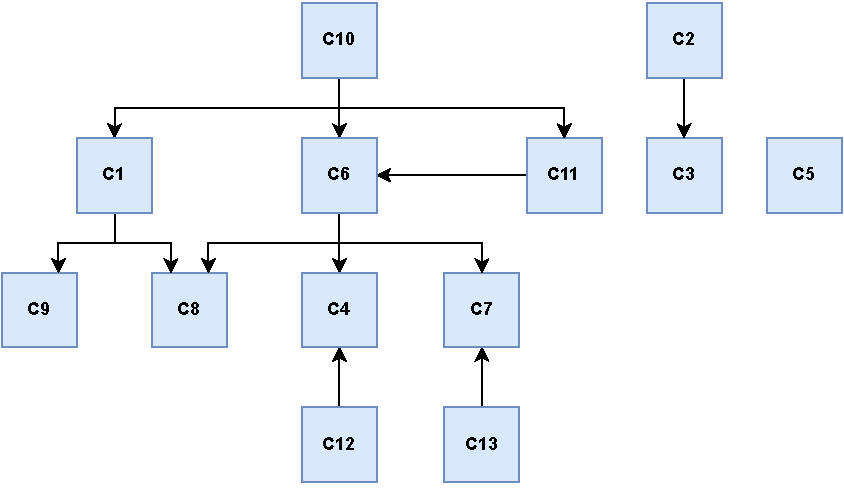
\includegraphics[width=0.87\linewidth]{figures/concept2concept.pdf}
    \caption[Dependencies between Conceptual Models]{Dependencies between
        Conceptual Models (Section~\ref{sec_conceptual})}
    \label{fig:conceptualdependencies}
\end{figure}
\vspace*{\fill}

\vspace*{\fill}
\begin{figure}[tbh]
    \centering
    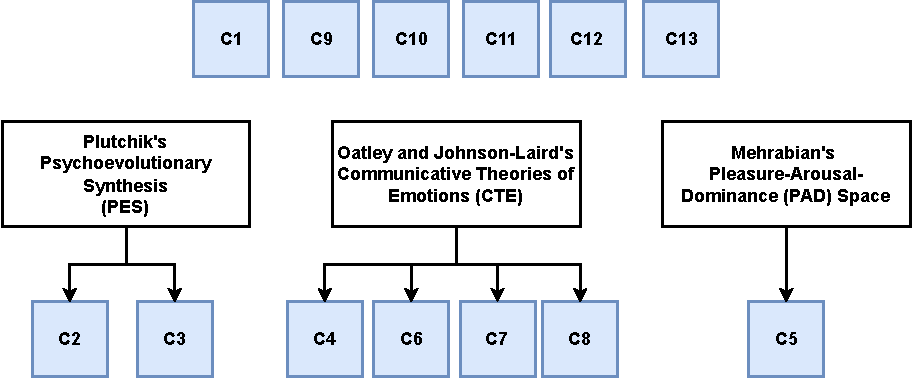
\includegraphics[width=\linewidth]{figures/theories2concept.pdf}
    \caption[Conceptual Model Dependencies on Affective
    Theories/Models]{Conceptual Model Dependencies on Affective Theories/Models
    (Section~\ref{sec_conceptual})}
    \label{fig:theories2conceptual}
\end{figure}
\vspace*{\fill}

\begin{figure}[tbh]
    \centering
    \includegraphics[height=0.96\textheight]{figures/assumptions2All.pdf}
    \caption[Dependencies on Assumptions]{Dependencies on Assumptions (Orange)
    (Section~\ref{sec_assumptions})}
    \label{fig:A2All}
\end{figure}

\begin{landscape}
    \begin{figure}[tbh]
        \centering
        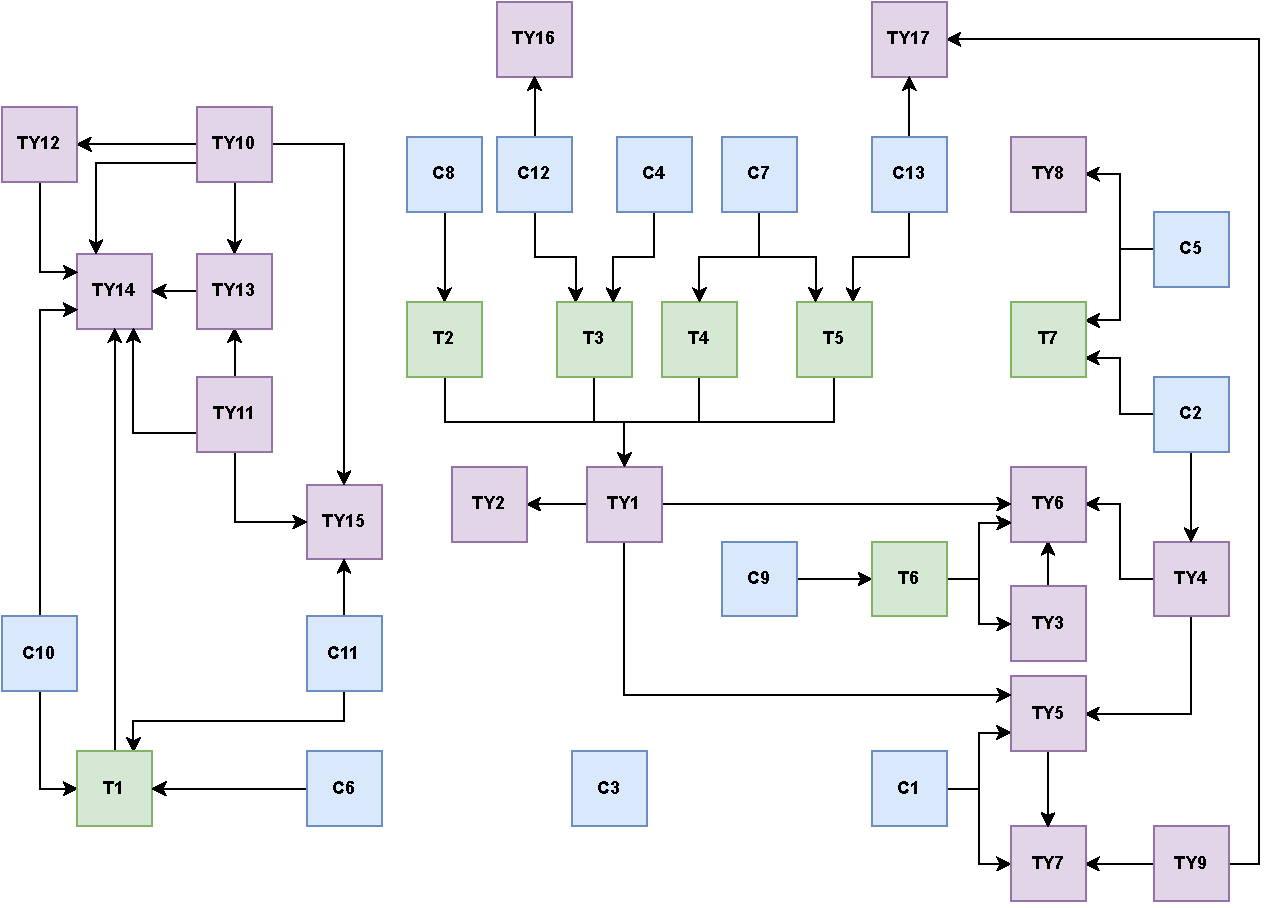
\includegraphics[width=\linewidth]{figures/concept2types_revised.pdf}
        \caption[Traceability between Theoretical Models and Data Types, and
        their dependencies on Conceptual Models]{Traceability between
        Theoretical Models (Green) and Data Types (Purple), and their
        dependencies on Conceptual Models (Blue)
        (Sections~\ref{sec_theoretical}, \ref{sec_typedefs},
        and~\ref{sec_conceptual})}
        \label{fig:C2TY}
    \end{figure}
\end{landscape}

\begin{landscape}
    \begin{figure}[tbh]
        \centering
        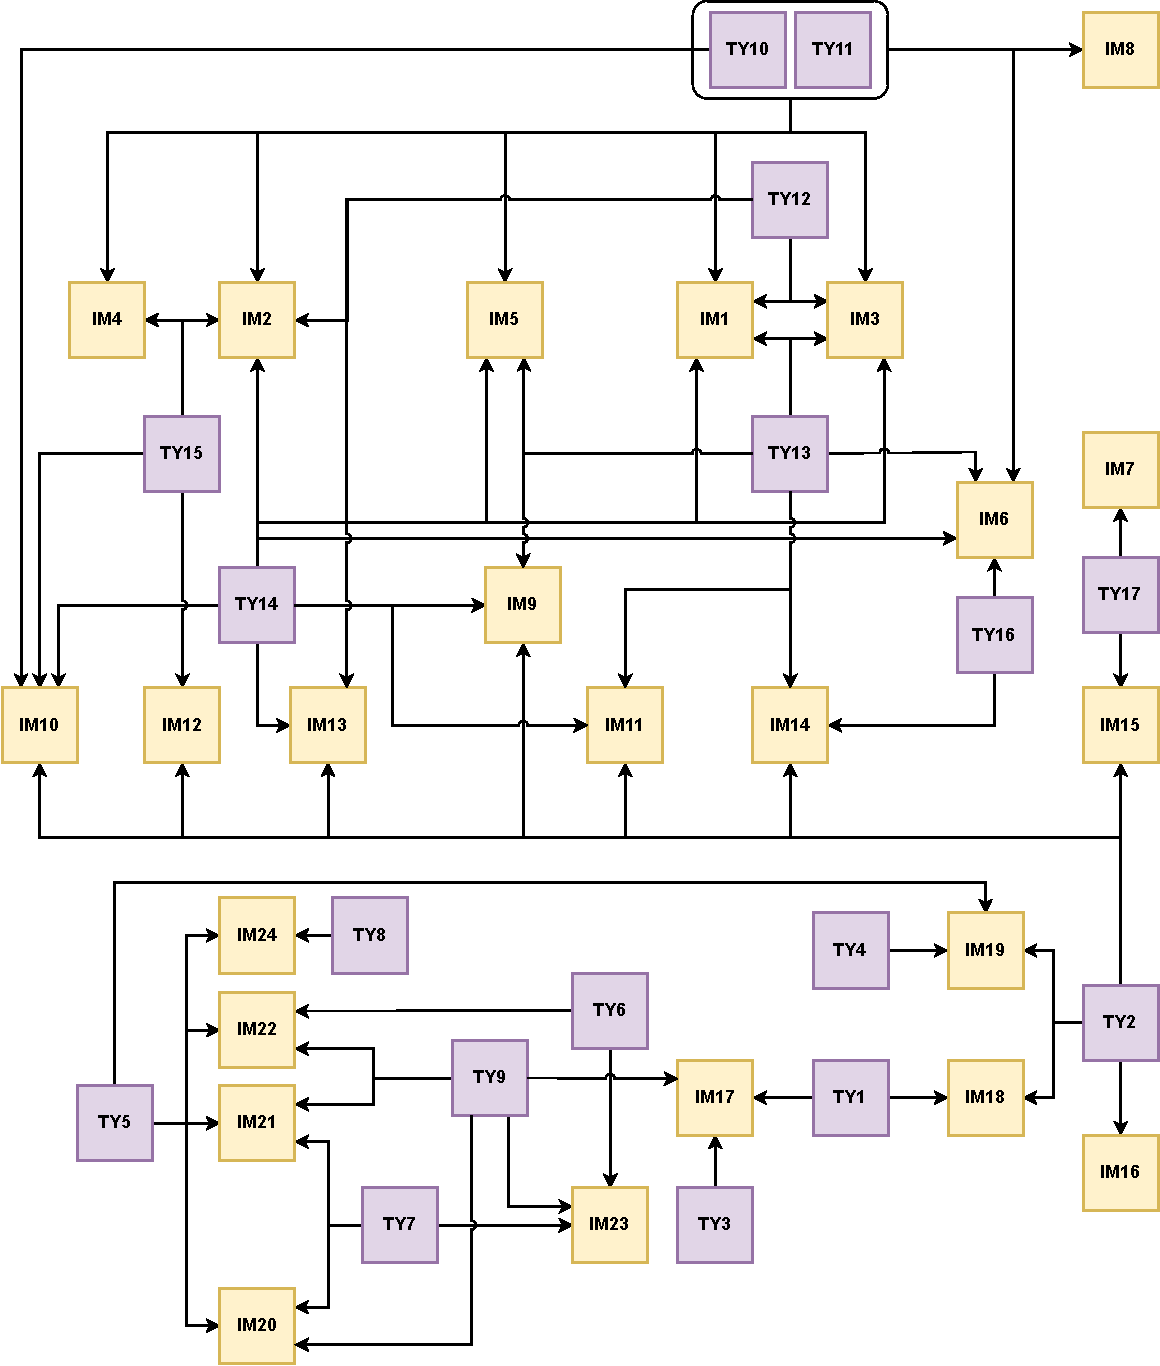
\includegraphics[width=0.88\linewidth]{figures/types2instance.pdf}
        \caption[Instance Models and their Dependencies on Theoretical Models
        and Data Types]{Instance Models (Yellow) and their Dependencies on
        Theoretical Models (Green) and Data Types (Purple)
        (Sections~\ref{sec_theoretical}, \ref{sec_typedefs},
        and~\ref{sec_instance})}
        \label{fig:T-TY2IM}
    \end{figure}
\end{landscape}

\vspace*{\fill}
\begin{figure}[tbh]
    \centering
    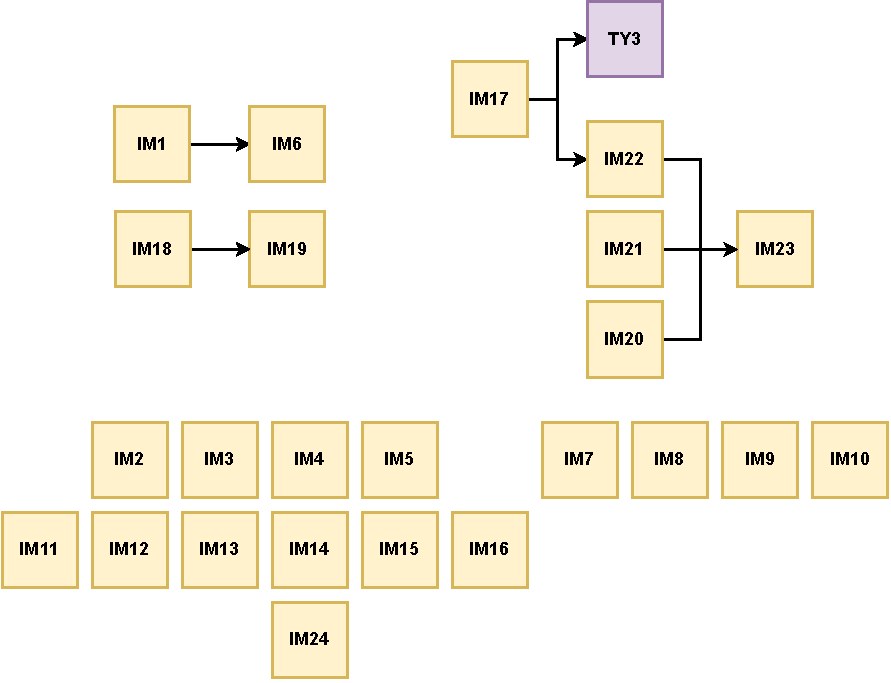
\includegraphics[width=0.5\linewidth]{figures/instance2instance.pdf}
    \caption[Dependencies between Instance Models]{Dependencies between
        Instance Models (Section~\ref{sec_instance})}
    \label{fig:IM}
\end{figure}
\vspace*{\fill}

\begin{figure}[tbh]
    \centering
    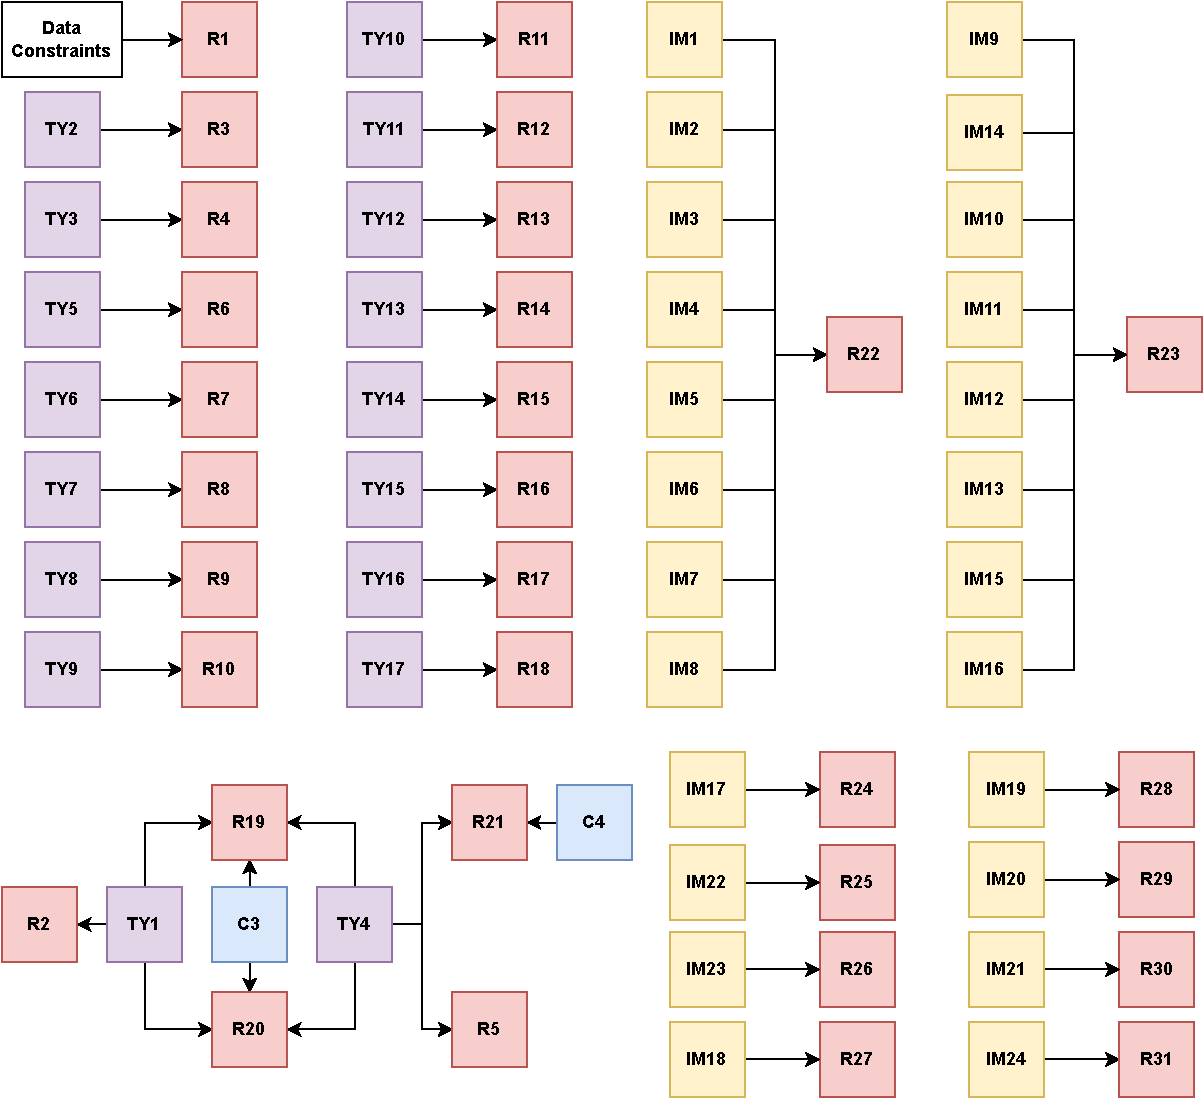
\includegraphics[width=\linewidth]{figures/reqs2All.pdf}
    \caption[Functional Requirements and their Dependencies on Conceptual
    Models, Data Types, Instance Models, and Data Constraints]{Functional
    Requirements (Red) and
    their Dependencies on Conceptual Models (Blue), Data Types (Purple),
    Instance Models (Yellow), and Data Constraints
    (Sections~\ref{sec_conceptual}, \ref{sec_typedefs}, \ref{sec_instance},
    \ref{sec_DataConstraints}, and \ref{sec_functionalreqs})}
    \label{fig:M2R}
\end{figure}

    \clearpage

    \section{Unit Test Description}
These tests exercise all functionality described in \progname{}'s Module
Interface Specification (Version~\misversion) not covered by the system-level
tests (Section~\ref{siutp_SystemTests}). They are organized by module.

\subsection{Tests for Functional Requirements}
\progname{}'s SRS clearly distinguishes between its data types and methods.
Therefore, the test plan separates tests into groups for \progname{}-defined
data types (Section~\ref{sec_sysDataTypes}) and methods
(Section~\ref{sec_sysMethods}).

\subsubsection{\progname{}-Defined Data Types}\label{sec_sysDataTypes}
These tests evaluate the correctness and precision of \progname{}-defined data
types as described in the SRS. Tests that check for adherence to data type
constraints (\rref{R_Types}) also address \progname{}'s response to recoverable
(Section~\ref{sec:sys-nf-recover}) %and non-recoverable
%(Section~\ref{sec:sys-nf-nonrecover})
 errors. Unless otherwise specified:
\begin{itemize}
    \item The NUnit Unit Testing Framework (Section~\ref{sec:tools}) automates
    all tests,
    \item Tests have an error tolerance $\epsilon = 1 \times 10^{-15}$, and
    \item All user messages are printed to the console.
\end{itemize}

\noindent Section~\ref{sec_unitFunctional} describes tests of other functions
necessary to manipulate data types that are \textit{not} described in the SRS.

\paragraph{\thesubsubsection.1 Emotion Intensity $\emotionintensitytype$ and
Intensity Change
$\responsestrength$}\label{sec_IntensityAndIntensityChg}
These tests check the satisfaction of \rref{R_IntensityTypeUse},
\rref{R_IntensityChangeType}, and adherence to the constraints on
$\emotionintensitytype$ and $\responsestrength$ (\rref{R_Types}). This includes
testing their constructors and comparison methods.

\begin{enumerate}

    \item{systemtest-IntensityConstructor\_GivenPositiveNumber}
    \begin{table}[H]
        \centering
        \begin{tabular}{P{0.25\linewidth}P{0.6\linewidth}}
            \toprule
            \textbf{Initial State} & New Session \\
            \textbf{Input} & $5 : \mathbb{R}$ \\ \midrule
            \textbf{Expected Output} & $5 : \emotionintensitytype$ \\
            \textbf{User Message} & -- \\ \bottomrule
        \end{tabular}
    \end{table}

    \item{systemtest-IntensityConstructor\_GivenPositiveNumberWithDecimals-1}
    \begin{table}[H]
        \centering
        \begin{tabular}{P{0.25\linewidth}P{0.6\linewidth}}
            \toprule
            \textbf{Initial State} & New Session \\
            \textbf{Input} & $5.8 : \mathbb{R}$ \\ \midrule
            \textbf{Expected Output} & $5.8 : \emotionintensitytype$ \\
            \textbf{User Message} & -- \\ \bottomrule
        \end{tabular}
    \end{table}

    \clearpage

    \item{systemtest-IntensityConstructor\_GivenPositiveNumberWithDecimals-2}
    \begin{table}[H]
        \centering
        \begin{tabular}{P{0.25\linewidth}P{0.6\linewidth}}
            \toprule
            \textbf{Initial State} & New Session \\
            \textbf{Input} & $2.000000000000001 : \mathbb{R}$ \\ \midrule
            \textbf{Expected Output} & $2.000000000000001 :
            \emotionintensitytype$ \\
            \textbf{User Message} & -- \\ \bottomrule
        \end{tabular}
    \end{table}

    \item{systemtest-IntensityConstructor\_GivenZero}
    \begin{table}[H]
        \centering
        \begin{tabular}{P{0.25\linewidth}P{0.6\linewidth}}
            \toprule
            \textbf{Initial State} & New Session \\
            \textbf{Input} & $0 : \mathbb{R}$ \\ \midrule
            \textbf{Expected Output} & $0 : \emotionintensitytype$ \\
            \textbf{User Message} & -- \\ \bottomrule
        \end{tabular}
    \end{table}

    \item{systemtest-IntensityConstructor\_GivenNegativeNumber}
    \begin{table}[H]
        \centering
        \begin{tabular}{P{0.25\linewidth}P{0.6\linewidth}}
            \toprule
            \textbf{Initial State} & New Session \\
            \textbf{Input} & $-5 : \mathbb{R}$ \\ \midrule
            \textbf{Expected Output} & $0 : \emotionintensitytype$ \\
            \textbf{Test Case Derivation} & When given a negative value,
            \progname{} sets the intensity value to $0$ because values of
            $\emotionintensitytype$ must be $\geq 0$.\\
            \textbf{User Message} & \texttt{Warning: Value for emotion
            intensity is out of bounds. Clamping to the range [0, infty).} \\
            \bottomrule
        \end{tabular}
    \end{table}

    \item{systemtest-IntensityChgConstructor\_GivenPositiveNumber}
    \begin{table}[H]
        \centering
        \begin{tabular}{P{0.25\linewidth}P{0.6\linewidth}}
            \toprule
            \textbf{Initial State} & New Session \\
            \textbf{Input} & $5 : \mathbb{R}$ \\ \midrule
            \textbf{Expected Output} & $5 : \responsestrength$ \\
            \textbf{User Message} & -- \\ \bottomrule
        \end{tabular}
    \end{table}

    \item{systemtest-IntensityChgConstructor\_GivenPositiveNumberWithDecimals-1}
    \begin{table}[H]
        \centering
        \begin{tabular}{P{0.25\linewidth}P{0.6\linewidth}}
            \toprule
            \textbf{Initial State} & New Session \\
            \textbf{Input} & $5.8 : \mathbb{R}$ \\ \midrule
            \textbf{Expected Output} & $5.8 : \responsestrength$ \\
            \textbf{User Message} & -- \\ \bottomrule
        \end{tabular}
    \end{table}

    \clearpage

    \item{systemtest-IntensityChgConstructor\_GivenPositiveNumberWithDecimals-2}
    \begin{table}[H]
        \centering
        \begin{tabular}{P{0.25\linewidth}P{0.6\linewidth}}
            \toprule
            \textbf{Initial State} & New Session \\
            \textbf{Input} & $2.000000000000001 : \mathbb{R}$ \\ \midrule
            \textbf{Expected Output} & $2.000000000000001 : \responsestrength$
            \\
            \textbf{User Message} & -- \\ \bottomrule
        \end{tabular}
    \end{table}

    \item{systemtest-IntensityChgConstructor\_GivenZero}
    \begin{table}[H]
        \centering
        \begin{tabular}{P{0.25\linewidth}P{0.6\linewidth}}
            \toprule
            \textbf{Initial State} & New Session \\
            \textbf{Input} & $0 : \mathbb{R}$ \\ \midrule
            \textbf{Expected Output} & $0 : \responsestrength$ \\
            \textbf{User Message} & -- \\ \bottomrule
        \end{tabular}
    \end{table}

    \item{systemtest-IntensityChgConstructor\_GivenNegativeNumber}
    \begin{table}[H]
        \centering
        \begin{tabular}{P{0.25\linewidth}P{0.6\linewidth}}
            \toprule
            \textbf{Initial State} & New Session \\
            \textbf{Input} & $-5 : \mathbb{R}$ \\ \midrule
            \textbf{Expected Output} & $-5 : \responsestrength$ \\
            \textbf{User Message} & -- \\ \bottomrule
        \end{tabular}
    \end{table}



    \item{systemtest-IntensityChgConstructor\_GivenNegativeNumberWithDecimals}
    \begin{table}[H]
        \centering
        \begin{tabular}{P{0.25\linewidth}P{0.6\linewidth}}
            \toprule
            \textbf{Initial State} & New Session \\
            \textbf{Input} & $-1.000000000000007 : \mathbb{R}$ \\ \midrule
            \textbf{Expected Output} & $-1.000000000000007 : \responsestrength$
            \\
            \textbf{User Message} & -- \\ \bottomrule
        \end{tabular}
    \end{table}

    \item{systemtest-CompareToIntensity\_FirstIsLarger-1}
    \begin{table}[H]
        \centering
        \begin{tabular}{P{0.25\linewidth}P{0.6\linewidth}}
            \toprule
            \textbf{Initial State} & $\mathit{i1} : \emotionintensitytype = 5$,
            $\mathit{i2} : \emotionintensitytype = 1$ \\
            \textbf{Input} & $\mathit{i1}$.CompareToIntensity($\mathit{i2}$) \\
            \midrule
            \textbf{Expected Output} & $1 : \mathbb{Z}$ \\
            \textbf{User Message} & -- \\ \bottomrule
        \end{tabular}
    \end{table}

    \item{systemtest-CompareToIntensity\_FirstIsLarger-2}
    \begin{table}[H]
        \centering
        \begin{tabular}{P{0.25\linewidth}P{0.6\linewidth}}
            \toprule
            \textbf{Initial State} & $\mathit{i1} : \emotionintensitytype = 5$,
            $\mathit{i2} : \emotionintensitytype = 2.1$ \\
            \textbf{Input} & $\mathit{i1}$.CompareToIntensity($\mathit{i2}$) \\
            \midrule
            \textbf{Expected Output} & $1 : \mathbb{Z}$ \\
            \textbf{User Message} & -- \\ \bottomrule
        \end{tabular}
    \end{table}

    \item{systemtest-CompareToIntensity\_FirstIsSmaller-1}
    \begin{table}[H]
        \centering
        \begin{tabular}{P{0.25\linewidth}P{0.6\linewidth}}
            \toprule
            \textbf{Initial State} & $\mathit{i1} : \emotionintensitytype = 1$,
            $\mathit{i2} : \emotionintensitytype = 5$ \\
            \textbf{Input} & $\mathit{i1}$.CompareToIntensity($\mathit{i2}$) \\
            \midrule
            \textbf{Expected Output} & $-1 : \mathbb{Z}$ \\
            \textbf{User Message} & -- \\ \bottomrule
        \end{tabular}
    \end{table}

    \item{systemtest-CompareToIntensity\_FirstIsSmaller-2}
    \begin{table}[H]
        \centering
        \begin{tabular}{P{0.25\linewidth}P{0.6\linewidth}}
            \toprule
            \textbf{Initial State} & $\mathit{i1} : \emotionintensitytype = 5$,
            $\mathit{i2} : \emotionintensitytype = 5.8$ \\
            \textbf{Input} & $\mathit{i1}$.CompareToIntensity($\mathit{i2}$) \\
            \midrule
            \textbf{Expected Output} & $-1 : \mathbb{Z}$ \\
            \textbf{User Message} & -- \\ \bottomrule
        \end{tabular}
    \end{table}

    \item{systemtest-CompareToIntensity\_FirstIsSmaller-3}
    \begin{table}[H]
        \centering
        \begin{tabular}{P{0.25\linewidth}P{0.6\linewidth}}
            \toprule
            \textbf{Initial State} & $\mathit{i1} : \emotionintensitytype = 2$,
            $\mathit{i2} : \emotionintensitytype = 2.000000000000001$ \\
            \textbf{Input} & $\mathit{i1}$.CompareToIntensity($\mathit{i2}$) \\
            \midrule
            \textbf{Expected Output} & $-1 : \mathbb{Z}$ \\
            \textbf{User Message} & -- \\ \bottomrule
        \end{tabular}
    \end{table}

    \item{systemtest-CompareToIntensity\_EqualValues}
    \begin{table}[H]
        \centering
        \begin{tabular}{P{0.25\linewidth}P{0.6\linewidth}}
            \toprule
            \textbf{Initial State} & $\mathit{i1} : \emotionintensitytype = 5$,
            $\mathit{i2} : \emotionintensitytype = 5$ \\
            \textbf{Input} & $\mathit{i1}$.CompareToIntensity($\mathit{i2}$) \\
            \midrule
            \textbf{Expected Output} & $0 : \mathbb{Z}$ \\
            \textbf{User Message} & -- \\ \bottomrule
        \end{tabular}
    \end{table}

    \item{systemtest-EqualsMinIntensity\_IntensityIsLarger-1}
    \begin{table}[H]
        \centering
        \begin{tabular}{P{0.25\linewidth}P{0.6\linewidth}}
            \toprule
            \textbf{Initial State} & $\mathit{i} : \emotionintensitytype = 5$,
            $\mathit{i_{min}} : \emotionintensitytype = 0$ \\
            \textbf{Input} & $\mathit{i}$.EqualsMinIntensity() \\ \midrule
            \textbf{Expected Output} & $\False : \mathbb{B}$ \\
            \textbf{User Message} & -- \\ \bottomrule
        \end{tabular}
    \end{table}



    \item{systemtest-EqualsMinIntensity\_IntensityIsLarger-2}
    \begin{table}[H]
        \centering
        \begin{tabular}{P{0.25\linewidth}P{0.6\linewidth}}
            \toprule
            \textbf{Initial State} & $\mathit{i} : \emotionintensitytype$ =
            2.3, $\mathit{i_{min}} : \emotionintensitytype = 0$ \\
            \textbf{Input} & $\mathit{i}$.EqualsMinIntensity() \\ \midrule
            \textbf{Expected Output} & $\False : \mathbb{B}$ \\
            \textbf{User Message} & -- \\ \bottomrule
        \end{tabular}
    \end{table}

    \item{systemtest-EqualsMinIntensity\_IntensityIsLarger-3}
    \begin{table}[H]
        \centering
        \begin{tabular}{P{0.25\linewidth}P{0.6\linewidth}}
            \toprule
            \textbf{Initial State} & $\mathit{i} : \emotionintensitytype =
            0.000000000000001$, $\mathit{i_{min}} : \emotionintensitytype = 0$
            \\
            \textbf{Input} & $\mathit{i}$.EqualsMinIntensity() \\
            \midrule
            \textbf{Expected Output} & $\False : \mathbb{B}$ \\
            \textbf{User Message} & -- \\ \bottomrule
        \end{tabular}
    \end{table}

    \item{systemtest-EqualsMinIntensity\_IntensityIsMin}
    \begin{table}[H]
        \centering
        \begin{tabular}{P{0.25\linewidth}P{0.6\linewidth}}
            \toprule
            \textbf{Initial State} & $\mathit{i} : \emotionintensitytype = 0$,
            $\mathit{i_{min}} : \emotionintensitytype = 0$ \\
            \textbf{Input} & $\mathit{i}$.EqualsMinIntensity() \\
            \midrule
            \textbf{Expected Output} & $\True : \mathbb{B}$ \\
            \textbf{User Message} & -- \\ \bottomrule
        \end{tabular}
    \end{table}

    \item{systemtest-CompareToIntensityChg\_FirstIsLarger-1}
    \begin{table}[H]
        \centering
        \begin{tabular}{P{0.25\linewidth}P{0.6\linewidth}}
            \toprule
            \textbf{Initial State} & $\mathit{d1} : \responsestrength = 5$,
            $\mathit{d2} : \responsestrength = 0$ \\
            \textbf{Input} & $\mathit{d1}$.CompareToIntensityChg($\mathit{d2}$)
            \\ \midrule
            \textbf{Expected Output} & $1 : \mathbb{Z}$ \\
            \textbf{User Message} & -- \\ \bottomrule
        \end{tabular}
    \end{table}

    \item{systemtest-CompareToIntensityChg\_FirstIsLarger-2}
    \begin{table}[H]
        \centering
        \begin{tabular}{P{0.25\linewidth}P{0.6\linewidth}}
            \toprule
            \textbf{Initial State} & $\mathit{d1} : \responsestrength = 5.8$,
            $\mathit{d2} : \responsestrength = 2.1$ \\
            \textbf{Input} & $\mathit{d1}$.CompareToIntensityChg($\mathit{d2}$)
            \\ \midrule
            \textbf{Expected Output} & $1 : \mathbb{Z}$ \\
            \textbf{User Message} & -- \\ \bottomrule
        \end{tabular}
    \end{table}

    \item{systemtest-CompareToIntensityChg\_FirstIsLarger-3}
    \begin{table}[H]
        \centering
        \begin{tabular}{P{0.25\linewidth}P{0.6\linewidth}}
            \toprule
            \textbf{Initial State} & $\mathit{d1} : \responsestrength = 5.8$,
            $\mathit{d2} : \responsestrength = -1.7$ \\
            \textbf{Input} & $\mathit{d1}$.CompareToIntensityChg($\mathit{d2}$)
            \\ \midrule
            \textbf{Expected Output} & $1 : \mathbb{Z}$ \\
            \textbf{User Message} & -- \\ \bottomrule
        \end{tabular}
    \end{table}

    \item{systemtest-CompareToIntensityChg\_FirstIsSmaller-1}
    \begin{table}[H]
        \centering
        \begin{tabular}{P{0.25\linewidth}P{0.6\linewidth}}
            \toprule
            \textbf{Initial State} & $\mathit{d1} : \responsestrength = 0$,
            $\mathit{d2} : \responsestrength = 5$ \\
            \textbf{Input} & $\mathit{d1}$.CompareToIntensityChg($\mathit{d2}$)
            \\ \midrule
            \textbf{Expected Output} & $-1 : \mathbb{Z}$ \\
            \textbf{User Message} & -- \\ \bottomrule
        \end{tabular}
    \end{table}

    \item{systemtest-CompareToIntensityChg\_FirstIsSmaller-2}
    \begin{table}[H]
        \centering
        \begin{tabular}{P{0.25\linewidth}P{0.6\linewidth}}
            \toprule
            \textbf{Initial State} & $\mathit{d1} : \responsestrength = 5$,
            $\mathit{d2} : \responsestrength = 5.8$ \\
            \textbf{Input} & $\mathit{d1}$.CompareToIntensityChg($\mathit{d2}$)
            \\ \midrule
            \textbf{Expected Output} & $-1 : \mathbb{Z}$ \\
            \textbf{User Message} & -- \\ \bottomrule
        \end{tabular}
    \end{table}

    \item{systemtest-CompareToIntensityChg\_FirstIsSmaller-3}
    \begin{table}[H]
        \centering
        \begin{tabular}{P{0.25\linewidth}P{0.6\linewidth}}
            \toprule
            \textbf{Initial State} & $\mathit{d1} : \responsestrength = -1.7$,
            $\mathit{d2} : \responsestrength = 5.8$ \\
            \textbf{Input} & $\mathit{d1}$.CompareToIntensityChg($\mathit{d2}$)
            \\ \midrule
            \textbf{Expected Output} & $-1 : \mathbb{Z}$ \\
            \textbf{User Message} & -- \\ \bottomrule
        \end{tabular}
    \end{table}

    \item{systemtest-CompareToIntensityChg\_FirstIsSmaller-4}
    \begin{table}[H]
        \centering
        \begin{tabular}{P{0.25\linewidth}P{0.6\linewidth}}
            \toprule
            \textbf{Initial State} & $\mathit{d1} : \responsestrength = -1.7$,
            $\mathit{d2} : \responsestrength = 0$ \\
            \textbf{Input} & $\mathit{d1}$.CompareToIntensityChg($\mathit{d2}$)
            \\ \midrule
            \textbf{Expected Output} & $-1 : \mathbb{Z}$ \\
            \textbf{User Message} & -- \\ \bottomrule
        \end{tabular}
    \end{table}

    \item{systemtest-CompareToIntensityChg\_FirstIsSmaller-5}
    \begin{table}[H]
        \centering
        \begin{tabular}{P{0.25\linewidth}P{0.6\linewidth}}
            \toprule
            \textbf{Initial State} & $\mathit{d1} : \responsestrength = 5$,
            $\mathit{d2} : \responsestrength = 5.000000000000001$ \\
            \textbf{Input} & $\mathit{d1}$.CompareToIntensityChg($\mathit{d2}$)
            \\ \midrule
            \textbf{Expected Output} & $-1 : \mathbb{Z}$ \\
            \textbf{User Message} & -- \\ \bottomrule
        \end{tabular}
    \end{table}

    \item{systemtest-CompareIntensityChg\_EqualValues}
    \begin{table}[H]
        \centering
        \begin{tabular}{P{0.25\linewidth}P{0.6\linewidth}}
            \toprule
            \textbf{Initial State} & $\mathit{d1} : \responsestrength = 5$,
            $\mathit{d2} : \responsestrength = 5$ \\
            \textbf{Input} & $\mathit{d1}$.CompareToIntensityChg($\mathit{d2}$)
            \\ \midrule
            \textbf{Expected Output} & $0 : \mathbb{Z}$ \\
            \textbf{User Message} & -- \\ \bottomrule
        \end{tabular}
    \end{table}


    \item{systemtest-CompareIntensityChgtoMinIntensity\_ChgIsLarger-1}
    \begin{table}[H]
        \centering
        \begin{tabular}{P{0.25\linewidth}P{0.6\linewidth}}
            \toprule
            \textbf{Initial State} & $\mathit{d} : \responsestrength = 5$,
            $\mathit{i_{min}} : \emotionintensitytype = 0$ \\
            \textbf{Input} & $\mathit{d}$.CompareToMinIntensity() \\ \midrule
            \textbf{Expected Output} & $1 : \mathbb{Z}$ \\
            \textbf{User Message} & -- \\ \bottomrule
        \end{tabular}
    \end{table}

    \item{systemtest-CompareIntensityChgtoMinIntensity\_ChgIsLarger-2}
    \begin{table}[H]
        \centering
        \begin{tabular}{P{0.25\linewidth}P{0.6\linewidth}}
            \toprule
            \textbf{Initial State} & $\mathit{d} : \responsestrength = 5.8$,
            $\mathit{i_{min}} : \emotionintensitytype = 0$ \\
            \textbf{Input} & $\mathit{d}$.CompareToMinIntensity() \\ \midrule
            \textbf{Expected Output} & $1 : \mathbb{Z}$ \\
            \textbf{User Message} & -- \\ \bottomrule
        \end{tabular}
    \end{table}

    \item{systemtest-CompareIntensityChgtoMinIntensity\_ChgIsLarger-3}
    \begin{table}[H]
        \centering
        \begin{tabular}{P{0.25\linewidth}P{0.6\linewidth}}
            \toprule
            \textbf{Initial State} & $\mathit{d} : \responsestrength = 2.1$,
            $\mathit{i_{min}} : \emotionintensitytype = 0$ \\
            \textbf{Input} & $\mathit{d}$.CompareToMinIntensity() \\ \midrule
            \textbf{Expected Output} & $1 : \mathbb{Z}$ \\
            \textbf{User Message} & -- \\ \bottomrule
        \end{tabular}
    \end{table}

    \item{systemtest-CompareIntensityChgtoMinIntensity\_ChgIsSmaller-1}
    \begin{table}[H]
        \centering
        \begin{tabular}{P{0.25\linewidth}P{0.6\linewidth}}
            \toprule
            \textbf{Initial State} & $\mathit{d} : \responsestrength = -5$,
            $\mathit{i_{min}} : \emotionintensitytype = 0$ \\
            \textbf{Input} & $\mathit{d}$.CompareToMinIntensity() \\ \midrule
            \textbf{Expected Output} & $-1 : \mathbb{Z}$ \\
            \textbf{User Message} & -- \\ \bottomrule
        \end{tabular}
    \end{table}

    \item{systemtest-CompareIntensityChgtoMinIntensity\_ChgIsSmaller-2}
    \begin{table}[H]
        \centering
        \begin{tabular}{P{0.25\linewidth}P{0.6\linewidth}}
            \toprule
            \textbf{Initial State} & $\mathit{d} : \responsestrength = -1.7$,
            $\mathit{i_{min}} : \emotionintensitytype = 0$ \\
            \textbf{Input} & $\mathit{d}$.CompareToMinIntensity() \\ \midrule
            \textbf{Expected Output} & $-1 : \mathbb{Z}$ \\
            \textbf{User Message} & -- \\ \bottomrule
        \end{tabular}
    \end{table}

    \item{systemtest-CompareIntensityChgtoMinIntensity\_ChgIsSmaller-3}
    \begin{table}[H]
        \centering
        \begin{tabular}{P{0.25\linewidth}P{0.6\linewidth}}
            \toprule
            \textbf{Initial State} & $\mathit{d} : \responsestrength =
            -0.000000000000001$, $\mathit{i_{min}} : \emotionintensitytype = 0$
            \\
            \textbf{Input} & $\mathit{d}$.CompareToMinIntensity() \\ \midrule
            \textbf{Expected Output} & $-1 : \mathbb{Z}$ \\
            \textbf{User Message} & -- \\ \bottomrule
        \end{tabular}
    \end{table}

    \item{systemtest-CompareIntensityChgtoMinIntensity\_ChgIsEqual}
    \begin{table}[H]
        \centering
        \begin{tabular}{P{0.25\linewidth}P{0.6\linewidth}}
            \toprule
            \textbf{Initial State} & $\mathit{d} : \responsestrength = 0$,
            $\mathit{i_{min}} : \emotionintensitytype = 0$ \\
            \textbf{Input} & $\mathit{d}$.CompareToMinIntensity() \\ \midrule
            \textbf{Expected Output} & $0 : \mathbb{Z}$ \\
            \textbf{User Message} & -- \\ \bottomrule
        \end{tabular}
    \end{table}

\end{enumerate}

%\clearpage\paragraph{Emotion Decay Rate $\emotiondecaytype$} These tests check
%the satisfaction of \rref{R_IntensityDecayType} and adherence to the
%constraints on $\emotiondecaytype$ (\rref{R_Types}). This only includes testing
%its constructor.
%
%\begin{enumerate}
%
%    \item{systemtest-DecayRateConstructor1}
%    \begin{table}[H]
%        \centering
%        \begin{tabular}{P{0.25\linewidth}P{0.6\linewidth}}
%            \toprule
%            \textbf{Initial State} & New Session \\
%            \textbf{Input} & $5 : \mathbb{R}$ \\ \midrule
%            \textbf{Expected Output} & $ 5 : \emotiondecaytype$ \\
%            \textbf{User Message} & -- \\ \bottomrule
%        \end{tabular}
%    \end{table}
%
%    \item{systemtest-DecayRateConstructor2}
%    \begin{table}[H]
%        \centering
%        \begin{tabular}{P{0.25\linewidth}P{0.6\linewidth}}
%            \toprule
%            \textbf{Initial State} & New Session \\
%            \textbf{Input} & $2.000000000000001 : \mathbb{R}$ \\ \midrule
%            \textbf{Expected Output} & $ 2.000000000000001 : \emotiondecaytype$
%            \\
%            \textbf{User Message} & -- \\ \bottomrule
%        \end{tabular}
%    \end{table}
%
%    \item{systemtest-DecayRateConstructor3}
%    \begin{table}[H]
%        \centering
%        \begin{tabular}{P{0.25\linewidth}P{0.6\linewidth}}
%            \toprule
%            \textbf{Initial State} & New Session \\
%            \textbf{Input} & $0.000000000000001 : \mathbb{R}$ \\ \midrule
%            \textbf{Expected Output} & $ 0.000000000000001 : \emotiondecaytype$
%            \\
%            \textbf{User Message} & -- \\ \bottomrule
%        \end{tabular}
%    \end{table}
%
%    \item{systemtest-DecayRateConstructorZeroInput}
%    \begin{table}[H]
%        \centering
%        \begin{tabular}{P{0.25\linewidth}P{0.6\linewidth}}
%            \toprule
%            \textbf{Initial State} & New Session \\
%            \textbf{Input} & $0 : \mathbb{R}$ \\ \midrule
%            \textbf{Expected Output} & EM\_DECAY\_RATE\_DEFAULT $ :
%            \emotiondecaytype$ \\
%            \textbf{Test Case Derivation} & When given a negative value,
%            \progname{} sets the decay rate to the default rate because values
%            of $\emotiondecaytype$ must be $> 0$.\\
%            \textbf{User Message} & \texttt{Warning: Emotion cannot decay at a
%                rate of zero or less. Setting to default decay rate of
%                EM\_DECAY\_RATE\_DEFAULT.} \\ \bottomrule
%        \end{tabular}
%    \end{table}
%
%    \clearpage
%
%    \item{systemtest-DecayRateConstructorNegativeInput}
%    \begin{table}[H]
%        \centering
%        \begin{tabular}{P{0.25\linewidth}P{0.6\linewidth}}
%            \toprule
%            \textbf{Initial State} & New Session \\
%            \textbf{Input} & $-5 : \mathbb{R}$ \\ \midrule
%            \textbf{Expected Output} & EM\_DECAY\_RATE\_DEFAULT $ :
%            \emotiondecaytype$ \\
%            \textbf{Test Case Derivation} & When given a negative value,
%            \progname{} sets the decay rate to the default rate because values
%            of $\emotiondecaytype$ must be $> 0$.\\
%            \textbf{User Message} & \texttt{Warning: Emotion cannot decay at a
%                rate of zero or less. Setting to default decay rate of
%                EM\_DECAY\_RATE\_DEFAULT.} \\ \bottomrule
%        \end{tabular}
%    \end{table}
%
%\end{enumerate}
%
%\clearpage\paragraph{Emotion Kinds $\emotionkindstype$} These tests check the
%satisfaction of \rref{R_EmotionKindsType} and adherence to the constraints on
%$\emotionkindstype$ (\rref{R_Types}). This means testing for the presence of
%the expected type, count, and order of emotion kinds.
%
%\begin{enumerate}
%
%    \item{systemtest-JoyKind}
%    \begin{table}[H]
%        \centering
%        \begin{tabular}{P{0.25\linewidth}P{0.6\linewidth}}
%            \toprule
%            \textbf{Initial State} & New Session \\
%            \textbf{Input} & $\emotionkindstype[0] = \mathtt{Joy}$ \\ \midrule
%            \textbf{Expected Output} & $ \True : \mathbb{B}$ \\
%            \textbf{User Message} & -- \\ \bottomrule
%        \end{tabular}
%    \end{table}
%
%    \item{systemtest-SadnessKind}
%    \begin{table}[H]
%        \centering
%        \begin{tabular}{P{0.25\linewidth}P{0.6\linewidth}}
%            \toprule
%            \textbf{Initial State} & New Session \\
%            \textbf{Input} & $\emotionkindstype[1] = \mathtt{Sadness}$ \\
%            \midrule
%            \textbf{Expected Output} & $ \True : \mathbb{B}$ \\
%            \textbf{User Message} & -- \\ \bottomrule
%        \end{tabular}
%    \end{table}
%
%    \item{systemtest-AngerKind}
%    \begin{table}[H]
%        \centering
%        \begin{tabular}{P{0.25\linewidth}P{0.6\linewidth}}
%            \toprule
%            \textbf{Initial State} & New Session \\
%            \textbf{Input} & $\emotionkindstype[2] = \mathtt{Anger}$ \\
%\midrule
%            \textbf{Expected Output} & $ \True : \mathbb{B}$ \\
%            \textbf{User Message} & -- \\ \bottomrule
%        \end{tabular}
%    \end{table}
%
%    \item{systemtest-FearKind}
%    \begin{table}[H]
%        \centering
%        \begin{tabular}{P{0.25\linewidth}P{0.6\linewidth}}
%            \toprule
%            \textbf{Initial State} & New Session \\
%            \textbf{Input} & $\emotionkindstype[3] = \mathtt{Fear}$ \\ \midrule
%            \textbf{Expected Output} & $ \True : \mathbb{B}$ \\
%            \textbf{User Message} & -- \\ \bottomrule
%        \end{tabular}
%    \end{table}
%
%    \item{systemtest-DisgustKind}
%    \begin{table}[H]
%        \centering
%        \begin{tabular}{P{0.25\linewidth}P{0.6\linewidth}}
%            \toprule
%            \textbf{Initial State} & New Session \\
%            \textbf{Input} & $\emotionkindstype[4] = \mathtt{Disgust}$ \\
%            \midrule
%            \textbf{Expected Output} & $ \True : \mathbb{B}$ \\
%            \textbf{User Message} & -- \\ \bottomrule
%        \end{tabular}
%    \end{table}
%
%    \clearpage
%
%    \item{systemtest-AcceptanceKind}
%    \begin{table}[H]
%        \centering
%        \begin{tabular}{P{0.25\linewidth}P{0.6\linewidth}}
%            \toprule
%            \textbf{Initial State} & New Session \\
%            \textbf{Input} & $\emotionkindstype[5] = \mathtt{Acceptance}$ \\
%            \midrule
%            \textbf{Expected Output} & $ \True : \mathbb{B}$ \\
%            \textbf{User Message} & -- \\ \bottomrule
%        \end{tabular}
%    \end{table}
%
%    \item{systemtest-SurpriseKind}
%    \begin{table}[H]
%        \centering
%        \begin{tabular}{P{0.25\linewidth}P{0.6\linewidth}}
%            \toprule
%            \textbf{Initial State} & New Session \\
%            \textbf{Input} & $\emotionkindstype[6] = \mathtt{Surprise}$ \\
%            \midrule
%            \textbf{Expected Output} & $ \True : \mathbb{B}$ \\
%            \textbf{User Message} & -- \\ \bottomrule
%        \end{tabular}
%    \end{table}
%
%    \item{systemtest-InterestKind}
%    \begin{table}[H]
%        \centering
%        \begin{tabular}{P{0.25\linewidth}P{0.6\linewidth}}
%            \toprule
%            \textbf{Initial State} & New Session \\
%            \textbf{Input} & $\emotionkindstype[7] = \mathtt{Interest}$ \\
%            \midrule
%            \textbf{Expected Output} & $ \True : \mathbb{B}$ \\
%            \textbf{User Message} & -- \\ \bottomrule
%        \end{tabular}
%    \end{table}
%
%    \item{systemtest-KindCount}
%    \begin{table}[H]
%        \centering
%        \begin{tabular}{P{0.25\linewidth}P{0.6\linewidth}}
%            \toprule
%            \textbf{Initial State} & New Session \\
%            \textbf{Input} & $| \emotionkindstype | = 8 $ \\ \midrule
%            \textbf{Expected Output} & $ \True : \mathbb{B}$ \\
%            \textbf{Test Case Derivation} & An additional test to ensure there
%            are no more than the eight expected emotion kinds. \\
%            \textbf{User Message} & -- \\ \bottomrule
%        \end{tabular}
%    \end{table}
%
%\end{enumerate}
%
%\clearpage\paragraph{Emotion State
%$\emotionstatetype$}\label{sec:sys-datatypes-emotionstate} These tests check
%the
%satisfaction of \rref{R_EmotionStateType} and adherence to the constraints on
%$\emotionstatetype$ (\rref{R_Types}). This only includes testing its
%constructor.
%
%\begin{enumerate}
%
%    \item{systemtest-EmotionStateConstructor}
%    \begin{table}[H]
%        \centering
%        \begin{tabular}{P{0.25\linewidth}P{0.6\linewidth}}
%            \toprule
%            \textbf{Initial State} & New Session \\
%            \textbf{Input} & $i = \langle \, 2 : \emotionintensitytype, 3.8 :
%            \emotionintensitytype, 40.89 : \emotionintensitytype, 67.3 :
%            \emotionintensitytype, 89.3 : \emotionintensitytype, 34.678 :
%            \emotionintensitytype,$ $ 4.678 : \emotionintensitytype, 78.4 :
%            \emotionintensitytype \, \rangle$, \newline $m = \langle \, 16 :
%            \emotionintensitytype, 10 : \emotionintensitytype, 100 :
%            \emotionintensitytype, 100.536 : \emotionintensitytype, 140.2 :
%            \emotionintensitytype,$ $ 50.7: \emotionintensitytype, 40.78 :
%            \emotionintensitytype, 80.234 : \emotionintensitytype \, \rangle$
%            \\ \midrule
%            \textbf{Expected Output} & $ \{ \mathit{intensities} = i,
%            \mathit{max} = m \} : \emotionstatetype $ \\
%            \textbf{User Message} & -- \\ \bottomrule
%        \end{tabular}
%    \end{table}
%
%    \item{systemtest-EmotionStateConstructorFirstIValueExceedsMValue}
%    \begin{table}[H]
%        \centering
%        \begin{tabular}{P{0.25\linewidth}P{0.6\linewidth}}
%            \toprule
%            \textbf{Initial State} & New Session \\
%            \textbf{Input} & $i = \langle \, 16.1 : \emotionintensitytype, 3.8
%:
%            \emotionintensitytype, 40.89 : \emotionintensitytype, 67.3 :
%            \emotionintensitytype, 89.3 : \emotionintensitytype, 34.678 :
%            \emotionintensitytype,$ $ 4.678 : \emotionintensitytype, 78.4 :
%            \emotionintensitytype \, \rangle$, \newline $m = \langle \, 16 :
%            \emotionintensitytype, 10 : \emotionintensitytype, 100 :
%            \emotionintensitytype, 100.536 : \emotionintensitytype, 140.2 :
%            \emotionintensitytype,$ $ 50.7: \emotionintensitytype, 40.78 :
%            \emotionintensitytype, 80.234 : \emotionintensitytype \, \rangle$
%            \\ \midrule
%            \textbf{Expected Output} & $ \{ \mathit{intensities} = i',
%            \mathit{max} = m \} : \emotionstatetype $, \newline where $i' = i$
%            with $i[0] = m[0]$ \\
%            \textbf{Test Case Derivation} & If $i.k > m.k$, \progname{} sets
%            $\mathit{intensities}.k$ to $m.k$ so that the invariant
%            $\mathit{intensities}.k < \mathit{max}.k$ holds. \\
%            \textbf{User Message} & \texttt{Warning: Value for
%            $\emotionkindstype[0]$ intensity is out of bounds. Clamping to the
%            range [$i[0].$MIN\_INTENTISTY, $m[0]$].} \\ \bottomrule
%        \end{tabular}
%    \end{table}
%
%    \clearpage
%
%    \item{systemtest-EmotionStateConstructorMultiIValueExceedsMValue}
%    \begin{table}[H]
%        \centering
%        \begin{tabular}{P{0.25\linewidth}P{0.6\linewidth}}
%            \toprule
%            \textbf{Initial State} & New Session \\
%            \textbf{Input} & $i = \langle \, 2 : \emotionintensitytype, 3.8 :
%            \emotionintensitytype, 101 : \emotionintensitytype, 67.3 :
%            \emotionintensitytype, 89.3 : \emotionintensitytype, 34.678 :
%            \emotionintensitytype,$ $ 4.678 : \emotionintensitytype, 80.235 :
%            \emotionintensitytype \, \rangle$, \newline $m = \langle \, 16 :
%            \emotionintensitytype, 10 : \emotionintensitytype, 100 :
%            \emotionintensitytype, 100.536 : \emotionintensitytype, 140.2 :
%            \emotionintensitytype,50.7: \emotionintensitytype,$ $  40.78 :
%            \emotionintensitytype, 80.234 : \emotionintensitytype \, \rangle$
%            \\ \midrule
%            \textbf{Expected Output} & $ \{ \mathit{intensities} = i',
%            \mathit{max} = m \} : \emotionstatetype $, \newline where $i' = i$
%            with $i[2] = m[2]$ \\
%            \textbf{Test Case Derivation} & If $i.k > m.k$, \progname{} sets
%            $\mathit{intensities}.k$ to $m.k$ so that the invariant
%            $\mathit{intensities}.k < \mathit{max}.k$ holds. \\
%            \textbf{User Message} & \texttt{Warning: Value for
%            $\emotionkindstype[2]$ intensity is out of bounds. Clamping to the
%            range [$i[2].$MIN\_INTENTISTY, $m[2]$].} \newline
%           \texttt{Warning: Value for $\emotionkindstype[7]$ intensity is out
%           of bounds. Clamping to the range [$i[7].$MIN\_INTENTISTY, $m[7]$].}
%           \\ \bottomrule
%        \end{tabular}
%    \end{table}
%
%    \item{systemtest-EmotionStateConstructorTooFewIntensitiesinI}
%    \begin{table}[H]
%        \centering
%        \begin{tabular}{P{0.25\linewidth}P{0.6\linewidth}}
%            \toprule
%            \textbf{Initial State} & New Session \\
%            \textbf{Input} & $i = \langle \, 2 : \emotionintensitytype, 3.8 :
%            \emotionintensitytype, 40.89 : \emotionintensitytype, 67.3 :
%            \emotionintensitytype, 89.3 : \emotionintensitytype, 34.678 :
%            \emotionintensitytype,$ $ 78.4 : \emotionintensitytype \, \rangle$,
%            \newline $m = \langle \, 16 : \emotionintensitytype, 10 :
%            \emotionintensitytype, 100 : \emotionintensitytype, 100.536 :
%            \emotionintensitytype, 140.2 : \emotionintensitytype,$ $ 50.7:
%            \emotionintensitytype, 40.78 : \emotionintensitytype, 80.234 :
%            \emotionintensitytype \, \rangle$ \\ \midrule
%            \textbf{Expected Output} & $ \{ \mathit{intensities} =
%            \mathtt{null}, \mathit{max} = \mathtt{null} \} : \emotionstatetype
%            $ \\
%            \textbf{Test Case Derivation} & The function $\emotionkindstype
%            \rightarrow \emotionintensitytype$ expects that there are exactly
%            the same number of values in $\emotionintensitytype$ as
%            $\emotionkindstype$. There is no way to know which values the user
%            intended to provide, so \progname{} makes no changes to
%            $\emotionstatetype$. \\
%            \textbf{User Message} & \texttt{Error: 7 intensity values given,
%            but there are exactly 8 types in the emotion state. Emotion state
%            intensities are unchanged.} \\ \bottomrule
%        \end{tabular}
%    \end{table}
%
%    \clearpage
%
%    \item{systemtest-EmotionStateConstructorTooManyIntensitiesinI}
%    \begin{table}[H]
%        \centering
%        \begin{tabular}{P{0.25\linewidth}P{0.6\linewidth}}
%            \toprule
%            \textbf{Initial State} & New Session \\
%            \textbf{Input} & $i = \langle \, 2 : \emotionintensitytype, 3.8 :
%            \emotionintensitytype, 40.89 : \emotionintensitytype, 67.3 :
%            \emotionintensitytype, 89.3 : \emotionintensitytype, 34.678 :
%            \emotionintensitytype,$ $ 4.678 : \emotionintensitytype, 78.4 :
%            \emotionintensitytype, 78.4 : \emotionintensitytype \, \rangle$,
%            \newline $m = \langle \, 16 : \emotionintensitytype, 10 :
%            \emotionintensitytype, 100 : \emotionintensitytype, 100.536 :
%            \emotionintensitytype, 140.2 : \emotionintensitytype,$ $ 50.7:
%            \emotionintensitytype, 40.78 : \emotionintensitytype, 80.234 :
%            \emotionintensitytype \, \rangle$ \\ \midrule
%            \textbf{Expected Output} & $ \{ \mathit{intensities} =
%            \mathtt{null}, \mathit{max} = \mathtt{null} \} : \emotionstatetype
%            $ \\
%            \textbf{Test Case Derivation} & The function $\emotionkindstype
%            \rightarrow \emotionintensitytype$ expects that there are exactly
%            the same number of values in $\emotionintensitytype$ as
%            $\emotionkindstype$. There is no way to know which values the user
%            intended to provide, so \progname{} makes no changes to
%            $\emotionstatetype$. \\
%            \textbf{User Message} & \texttt{Error: 9 intensity values given,
%            but there are exactly 8 types in the emotion state. Emotion state
%            intensities are unchanged.} \\ \bottomrule
%        \end{tabular}
%    \end{table}
%
%    \item{systemtest-EmotionStateConstructorTooFewIntensitiesinM}
%    \begin{table}[H]
%        \centering
%        \begin{tabular}{P{0.25\linewidth}P{0.6\linewidth}}
%            \toprule
%            \textbf{Initial State} & New Session \\
%            \textbf{Input} & $i = \langle \, 2 : \emotionintensitytype, 3.8 :
%            \emotionintensitytype, 40.89 : \emotionintensitytype, 67.3 :
%            \emotionintensitytype, 89.3 : \emotionintensitytype, 34.678 :
%            \emotionintensitytype,$ $ 4.678 : \emotionintensitytype, 78.4 :
%            \emotionintensitytype \, \rangle$, \newline $m = \langle \, 16 :
%            \emotionintensitytype, 10 : \emotionintensitytype, 100 :
%            \emotionintensitytype, 100.536 : \emotionintensitytype, 140.2 :
%            \emotionintensitytype,$ $ 50.7: \emotionintensitytype, 40.78 :
%            \emotionintensitytype \, \rangle$ \\ \midrule
%            \textbf{Expected Output} & $ \{ \mathit{intensities} =
%            \mathtt{null}, \mathit{max} = \mathtt{null} \} : \emotionstatetype
%            $ \\
%            \textbf{Test Case Derivation} & The function $\emotionkindstype
%            \rightarrow \emotionintensitytype$ expects that there are exactly
%            the same number of values in $\emotionintensitytype$ as
%            $\emotionkindstype$. There is no way to know which values the user
%            intended to provide, so \progname{} makes no changes to
%            $\emotionstatetype$. \\
%            \textbf{User Message} & \texttt{Error: 7 maximum values given, but
%            there are exactly 8 types in the emotion state. Emotion state max
%            intensities are unchanged.} \\ \bottomrule
%        \end{tabular}
%    \end{table}
%
%    \clearpage
%
%    \item{systemtest-EmotionStateConstructorTooManyIntensitiesinM}
%    \begin{table}[H]
%        \centering
%        \begin{tabular}{P{0.25\linewidth}P{0.6\linewidth}}
%            \toprule
%            \textbf{Initial State} & New Session \\
%            \textbf{Input} & $i = \langle \, 2 : \emotionintensitytype, 3.8 :
%            \emotionintensitytype, 40.89 : \emotionintensitytype, 67.3 :
%            \emotionintensitytype, 89.3 : \emotionintensitytype, 34.678 :
%            \emotionintensitytype,$ $ 4.678 : \emotionintensitytype, 78.4 :
%            \emotionintensitytype \, \rangle$, \newline $m = \langle \, 16 :
%            \emotionintensitytype, 10 : \emotionintensitytype, 100 :
%            \emotionintensitytype, 100.536 : \emotionintensitytype, 140.2 :
%            \emotionintensitytype,$ $ 50.7: \emotionintensitytype, 40.78 :
%            \emotionintensitytype, 80.234 : \emotionintensitytype, 80.234 :
%            \emotionintensitytype \, \rangle$ \\ \midrule
%            \textbf{Expected Output} & $ \{ \mathit{intensities} =
%            \mathtt{null}, \mathit{max} = \mathtt{null} \} : \emotionstatetype
%            $ \\
%            \textbf{Test Case Derivation} & The function $\emotionkindstype
%            \rightarrow \emotionintensitytype$ expects that there are exactly
%            the same number of values in $\emotionintensitytype$ as
%            $\emotionkindstype$. There is no way to know which values the user
%            intended to provide, so \progname{} makes no changes to
%            $\emotionstatetype$. \\
%            \textbf{User Message} & \texttt{Error: 9 maximum values given, but
%            there are exactly 8 types in the emotion state. Emotion state max
%            intensities are unchanged.} \\ \bottomrule
%        \end{tabular}
%    \end{table}
%
%\end{enumerate}
%
%\clearpage\paragraph{Emotion Decay State $\emotionstatedecaytype$} These tests
%check the satisfaction of \rref{R_EmotionDecayStateType} and adherence to the
%constraints on $\emotionstatedecaytype$ (\rref{R_Types}). This only includes
%testing its constructor (?).
%
%\clearpage\paragraph{Emotion $\emotiontype$} These tests check the satisfaction
%of \rref{R_EmotionType} and adherence to the constraints on $\emotiontype$
%(\rref{R_Types}). This only includes testing its constructor (?).
%
%\clearpage\paragraph{PAD Point $\padpoint$} These tests check the satisfaction
%of \rref{R_PADPointType} and adherence to the constraints on $\padpoint$
%(\rref{R_Types}). This only includes testing its constructor.
%
%\begin{enumerate}
%
%    \item{systemtest-PADPntConstructor1}
%    \begin{table}[H]
%        \centering
%        \begin{tabular}{P{0.25\linewidth}P{0.6\linewidth}}
%            \toprule
%            \textbf{Initial State} & New Session \\
%            \textbf{Input} & $-1 : \mathbb{R}$, $-1 : \mathbb{R}$, $-1 :
%            \mathbb{R}$ \\ \midrule
%            \textbf{Expected Output} & $(-1, -1, -1) : \padpoint$ \\
%            \textbf{User Message} & -- \\ \bottomrule
%        \end{tabular}
%    \end{table}
%
%    \item{systemtest-PADPntConstructor2}
%    \begin{table}[H]
%        \centering
%        \begin{tabular}{P{0.25\linewidth}P{0.6\linewidth}}
%            \toprule
%            \textbf{Initial State} & New Session \\
%            \textbf{Input} & $0 : \mathbb{R}$, $0 : \mathbb{R}$, $0 :
%            \mathbb{R}$ \\ \midrule
%            \textbf{Expected Output} & $(0, 0, 0) : \padpoint$ \\
%            \textbf{User Message} & -- \\ \bottomrule
%        \end{tabular}
%    \end{table}
%
%    \item{systemtest-PADPntConstructor3}
%    \begin{table}[H]
%        \centering
%        \begin{tabular}{P{0.25\linewidth}P{0.6\linewidth}}
%            \toprule
%            \textbf{Initial State} & New Session \\
%            \textbf{Input} & $1 : \mathbb{R}$, $1 : \mathbb{R}$, $1 :
%            \mathbb{R}$ \\ \midrule
%            \textbf{Expected Output} & $(1, 1, 1) : \padpoint$ \\
%            \textbf{User Message} & -- \\ \bottomrule
%        \end{tabular}
%    \end{table}
%
%    \item{systemtest-PADPntConstructor4}
%    \begin{table}[H]
%        \centering
%        \begin{tabular}{P{0.25\linewidth}P{0.6\linewidth}}
%            \toprule
%            \textbf{Initial State} & New Session \\
%            \textbf{Input} & $-0.000000000000001 : \mathbb{R}$,
%            $-0.000000000000001 : \mathbb{R}$, $-0.000000000000001 :
%            \mathbb{R}$ \\ \midrule
%            \textbf{Expected Output} & $(-0.000000000000001,
%            -0.000000000000001,$ $-0.000000000000001) : \padpoint$ \\
%            \textbf{User Message} & -- \\ \bottomrule
%        \end{tabular}
%    \end{table}
%
%    \item{systemtest-PADPntConstructor5}
%    \begin{table}[H]
%        \centering
%        \begin{tabular}{P{0.25\linewidth}P{0.6\linewidth}}
%            \toprule
%            \textbf{Initial State} & New Session \\
%            \textbf{Input} & $0.000000000000001 : \mathbb{R}$,
%            $0.000000000000001 : \mathbb{R}$, $0.000000000000001 :
%            \mathbb{R}$ \\ \midrule
%            \textbf{Expected Output} & $(0.000000000000001,
%            0.000000000000001,$ $0.000000000000001) : \padpoint$ \\
%            \textbf{User Message} & -- \\ \bottomrule
%        \end{tabular}
%    \end{table}
%
%    \item{systemtest-PADPntConstructor6}
%    \begin{table}[H]
%        \centering
%        \begin{tabular}{P{0.25\linewidth}P{0.6\linewidth}}
%            \toprule
%            \textbf{Initial State} & New Session \\
%            \textbf{Input} & $0.999999999999999 : \mathbb{R}$,
%            $0.999999999999999 : \mathbb{R}$, $0.999999999999999 :
%            \mathbb{R}$ \\ \midrule
%            \textbf{Expected Output} & $(0.999999999999999,
%            0.999999999999999,$ $0.999999999999999) : \padpoint$ \\
%            \textbf{User Message} & -- \\ \bottomrule
%        \end{tabular}
%    \end{table}
%
%    \item{systemtest-PADPntConstructor7}
%    \begin{table}[H]
%        \centering
%        \begin{tabular}{P{0.25\linewidth}P{0.6\linewidth}}
%            \toprule
%            \textbf{Initial State} & New Session \\
%            \textbf{Input} & $-0.999999999999999 : \mathbb{R}$,
%            $-0.999999999999999 : \mathbb{R}$, $-0.999999999999999 :
%            \mathbb{R}$ \\ \midrule
%            \textbf{Expected Output} & $(-0.999999999999999,
%            -0.999999999999999,$ $-0.999999999999999) : \padpoint$ \\
%            \textbf{User Message} & -- \\ \bottomrule
%        \end{tabular}
%    \end{table}
%
%    \item{systemtest-PADPntConstructorExceedMinBound}
%    \begin{table}[H]
%        \centering
%        \begin{tabular}{P{0.25\linewidth}P{0.6\linewidth}}
%            \toprule
%            \textbf{Initial State} & New Session \\
%            \textbf{Input} & $-1.000000000000001 : \mathbb{R}$,
%            $-1.000000000000001 : \mathbb{R}$, $-1.000000000000001 :
%            \mathbb{R}$ \\ \midrule
%            \textbf{Expected Output} & $(-1, -1, -1) : \padpoint$ \\
%            \textbf{Test Case Derivation} & When given values that are outside
%            the range $[-1, 1]$, \progname{} sets the dimension to the closest
%            bound.\\
%            \multirow{6}{*}{\textbf{User Message}} & \texttt{Warning: Value for
%            P dimension (-1.000000000000001) is out of bounds. Clamping to the
%            range [-1, 1].} \\
%            & \texttt{Warning: Value for A dimension (-1.000000000000001) is
%            out of bounds. Clamping to the range [-1, 1].} \\
%            & \texttt{Warning: Value for D dimension (-1.000000000000001) is
%            out of bounds. Clamping to the range [-1, 1].} \\ \bottomrule
%        \end{tabular}
%    \end{table}
%
%    \clearpage
%
%    \item{systemtest-PADPntConstructorExceedMaxBound}
%    \begin{table}[H]
%        \centering
%        \begin{tabular}{P{0.25\linewidth}P{0.6\linewidth}}
%            \toprule
%            \textbf{Initial State} & New Session \\
%            \textbf{Input} & $1.000000000000001 : \mathbb{R}$,
%            $1.000000000000001 : \mathbb{R}$, $1.000000000000001 :
%            \mathbb{R}$ \\ \midrule
%            \textbf{Expected Output} & $(1, 1, 1) : \padpoint$ \\
%            \textbf{Test Case Derivation} & When given values that are outside
%            the range $[-1, 1]$, \progname{} sets the dimension to the closest
%            bound.\\
%            \multirow{6}{*}{\textbf{User Message}} & \texttt{Warning: Value for
%            P dimension (1.000000000000001) is out of bounds. Clamping to the
%            range [-1, 1].} \\
%            & \texttt{Warning: Value for A dimension (1.000000000000001) is out
%            of bounds. Clamping to the range [-1, 1].} \\
%            & \texttt{Warning: Value for D dimension (1.000000000000001) is out
%            of bounds. Clamping to the range [-1, 1].} \\ \bottomrule
%        \end{tabular}
%    \end{table}
%
%    \item{systemtest-PADPntConstructorExceedBoundsMixed}
%    \begin{table}[H]
%        \centering
%        \begin{tabular}{P{0.25\linewidth}P{0.6\linewidth}}
%            \toprule
%            \textbf{Initial State} & New Session \\
%            \textbf{Input} & $-0.000000000000001 : \mathbb{R}$,
%            $-1.000000000000001 : \mathbb{R}$, $1 : \mathbb{R}$ \\ \midrule
%            \textbf{Expected Output} & $(-0.000000000000001, -1,$ $1) :
%            \padpoint$ \\
%            \textbf{Test Case Derivation} & When given values that are outside
%            the range $[-1, 1]$, \progname{} sets the dimension to the closest
%            bound.\\
%            \textbf{User Message} & \texttt{Warning: Value for A dimension
%            (-1.000000000000001) is out of bounds. Clamping to the range [-1,
%            1].} \\ \bottomrule
%        \end{tabular}
%    \end{table}
%
%\end{enumerate}
%
%\clearpage\paragraph{Goal $\goaltype$} These tests check the satisfaction of
%\rref{R_GoalType} and adherence to the constraints on $\goaltype$
%(\rref{R_Types}).
%
%\clearpage\paragraph{Plan $\plantype$} These tests check the satisfaction of
%\rref{R_PlanType} and adherence to the constraints on $\plantype$
%(\rref{R_Types}).
%
%\clearpage\paragraph{Attention $\attentiontype$} These tests check the
%satisfaction of \rref{R_Attention} and adherence to the constraints on
%$\attentiontype$ (\rref{R_Types}). This only includes testing its constructor.
%
%\begin{enumerate}
%
%    \item{systemtest-AttentionConstructorPositiveStepSize1}
%    \begin{table}[H]
%        \centering
%        \begin{tabular}{P{0.25\linewidth}P{0.6\linewidth}}
%            \toprule
%            \textbf{Initial State} & New Session \\
%            \textbf{Input} & $5 : \mathbb{Z}$, $\mathit{dt} : \deltatimetype >
%            0$ \\ \midrule
%            \textbf{Expected Output} & $\{ 5, \mathit{dt} \} : \attentiontype$
%            \\
%            \textbf{User Message} & -- \\ \bottomrule
%        \end{tabular}
%    \end{table}
%
%    \item{systemtest-AttentionConstructorPositiveStepSize2}
%    \begin{table}[H]
%        \centering
%        \begin{tabular}{P{0.25\linewidth}P{0.6\linewidth}}
%            \toprule
%            \textbf{Initial State} & New Session \\
%            \textbf{Input} & $0 : \mathbb{Z}$, $\mathit{dt} : \deltatimetype >
%            0$ \\ \midrule
%            \textbf{Expected Output} & $\{ 0, \mathit{dt} \} : \attentiontype$
%            \\
%            \textbf{User Message} & -- \\ \bottomrule
%        \end{tabular}
%    \end{table}
%
%    \item{systemtest-AttentionConstructorZeroStepSize1}
%    \begin{table}[H]
%        \centering
%        \begin{tabular}{P{0.25\linewidth}P{0.6\linewidth}}
%            \toprule
%            \textbf{Initial State} & New Session \\
%            \textbf{Input} & $5 : \mathbb{Z}$, $\mathit{dt} : \deltatimetype =
%            0$ \\ \midrule
%            \textbf{Expected Output} & $\{ 5, \mathit{dt} \} : \attentiontype$
%            \\
%            \textbf{User Message} & -- \\ \bottomrule
%        \end{tabular}
%    \end{table}
%
%    \item{systemtest-AttentionConstructorZeroStepSize2}
%    \begin{table}[H]
%        \centering
%        \begin{tabular}{P{0.25\linewidth}P{0.6\linewidth}}
%            \toprule
%            \textbf{Initial State} & New Session \\
%            \textbf{Input} & $0 : \mathbb{Z}$, $\mathit{dt} : \deltatimetype =
%            0$ \\ \midrule
%            \textbf{Expected Output} & $\{ 0, \mathit{dt} \} : \attentiontype$
%            \\
%            \textbf{User Message} & -- \\ \bottomrule
%        \end{tabular}
%    \end{table}
%
%    \item{systemtest-AttentionConstructorPositiveStepSizeNegativeInput}
%    \begin{table}[H]
%        \centering
%        \begin{tabular}{P{0.25\linewidth}P{0.6\linewidth}}
%            \toprule
%            \textbf{Initial State} & New Session \\
%            \textbf{Input} & $-5 : \mathbb{Z}$, $\mathit{dt} : \deltatimetype >
%            0$ \\ \midrule
%            \textbf{Expected Output} & $\{ 0, \mathit{dt} \} : \attentiontype$
%            \\
%            \textbf{Test Case Derivation} & When given negative values for
%            elapsed steps, \progname{} sets it to 0 because allocated attention
%            cannot be negative.\\
%            \textbf{User Message} & \texttt{Warning: Cannot allocate fewer than
%                zero steps of attention. Setting to zero.} \\ \bottomrule
%        \end{tabular}
%    \end{table}
%
%    \clearpage
%
%    \item{systemtest-AttentionConstructorZeroStepSizeNegativeInput}
%    \begin{table}[H]
%        \centering
%        \begin{tabular}{P{0.25\linewidth}P{0.6\linewidth}}
%            \toprule
%            \textbf{Initial State} & New Session \\
%            \textbf{Input} & $-5 : \mathbb{Z}$, $\mathit{dt} : \deltatimetype =
%            0$ \\ \midrule
%            \textbf{Expected Output} & $\{ 0, \mathit{dt} \} : \attentiontype$
%            \\
%            \textbf{Test Case Derivation} & When given negative values for
%            elapsed steps, \progname{} sets it to 0 because allocated attention
%            cannot be negative.\\
%            \textbf{User Message} & \texttt{Warning: Cannot allocate fewer than
%                zero steps of attention. Setting to zero.} \\ \bottomrule
%        \end{tabular}
%    \end{table}
%
%    \item{systemtest-AttentionConstructorNegativeStepSize1}
%    \begin{table}[H]
%        \centering
%        \begin{tabular}{P{0.25\linewidth}P{0.6\linewidth}}
%            \toprule
%            \textbf{Initial State} & New Session \\
%            \textbf{Input} & $5 : \mathbb{Z}$, $\mathit{dt} : \deltatimetype <
%            0$ \\ \midrule
%            \textbf{Expected Output} & $\{ 5, 0 : \deltatimetype \} :
%            \attentiontype$ \\
%            \textbf{Test Case Derivation} & When given negative values for
%            step size, \progname{} sets it to 0 because attention grows by
%            default.\\
%            \textbf{User Message} & \texttt{Warning: Step size cannot be
%                negative. Setting to zero.} \\ \bottomrule
%        \end{tabular}
%    \end{table}
%
%    \item{systemtest-AttentionConstructorNegativeStepSize2}
%    \begin{table}[H]
%        \centering
%        \begin{tabular}{P{0.25\linewidth}P{0.6\linewidth}}
%            \toprule
%            \textbf{Initial State} & New Session \\
%            \textbf{Input} & $0 : \mathbb{Z}$, $\mathit{dt} : \deltatimetype <
%            0$ \\ \midrule
%            \textbf{Expected Output} & $\{ 0, 0 : \deltatimetype \} :
%            \attentiontype$ \\
%            \textbf{Test Case Derivation} & When given negative values for
%            step size, \progname{} sets it to 0 because attention grows by
%            default.\\
%            \textbf{User Message} & \texttt{Warning: Step size cannot be
%                negative. Setting to zero.} \\ \bottomrule
%        \end{tabular}
%    \end{table}
%
%    \item{systemtest-AttentionConstructorPositiveStepSize3}
%    \begin{table}[H]
%        \centering
%        \begin{tabular}{P{0.25\linewidth}P{0.6\linewidth}}
%            \toprule
%            \textbf{Initial State} & New Session \\
%            \textbf{Input} & $-5 : \mathbb{Z}$, $\mathit{dt} : \deltatimetype <
%            0$ \\ \midrule
%            \textbf{Expected Output} & $\{ 0, 0 : \deltatimetype \} :
%            \attentiontype$ \\
%            \textbf{Test Case Derivation} & When given negative values for
%            step size, \progname{} sets it to 0 because attention grows by
%            default.\\
%            \textbf{User Message} & \texttt{Warning: Cannot allocate fewer than
%                zero steps of attention. Setting to zero.} \newline
%            \texttt{Warning: Step size cannot be negative. Setting to zero.} \\
%            \bottomrule
%        \end{tabular}
%    \end{table}
%
%\end{enumerate}
%
%\clearpage
%
%\paragraph{Social Attachment $\socialattachmenttype$} These tests check the
%satisfaction of \rref{R_SocialAttachment} and adherence to the constraints on
%$\socialattachmenttype$ (\rref{R_Types}). This only includes testing its
%constructor.
%
%\begin{enumerate}
%
%    \item{systemtest-SocialAttachmentConstructor1}
%    \begin{table}[H]
%        \centering
%        \begin{tabular}{P{0.25\linewidth}P{0.6\linewidth}}
%            \toprule
%            \textbf{Initial State} & New Session \\
%            \textbf{Input} & $0 : \mathbb{Z}$ \\ \midrule
%            \textbf{Expected Output} & $0 : \socialattachmenttype$ \\
%            \textbf{User Message} & -- \\ \bottomrule
%        \end{tabular}
%    \end{table}
%
%    \item{systemtest-SocialAttachmentConstructor2}
%    \begin{table}[H]
%        \centering
%        \begin{tabular}{P{0.25\linewidth}P{0.6\linewidth}}
%            \toprule
%            \textbf{Initial State} & New Session \\
%            \textbf{Input} & $1 : \mathbb{Z}$ \\ \midrule
%            \textbf{Expected Output} & $1 : \socialattachmenttype$ \\
%            \textbf{User Message} & -- \\ \bottomrule
%        \end{tabular}
%    \end{table}
%
%    \item{systemtest-SocialAttachmentConstructor3}
%    \begin{table}[H]
%        \centering
%        \begin{tabular}{P{0.25\linewidth}P{0.6\linewidth}}
%            \toprule
%            \textbf{Initial State} & New Session \\
%            \textbf{Input} & $-1 : \mathbb{Z}$ \\ \midrule
%            \textbf{Expected Output} & $-1 : \socialattachmenttype$ \\
%            \textbf{User Message} & -- \\ \bottomrule
%        \end{tabular}
%    \end{table}
%
%    \item{systemtest-SocialAttachmentConstructor4}
%    \begin{table}[H]
%        \centering
%        \begin{tabular}{P{0.25\linewidth}P{0.6\linewidth}}
%            \toprule
%            \textbf{Initial State} & New Session \\
%            \textbf{Input} & max$(\mathbb{Z})$ \\ \midrule
%            \textbf{Expected Output} & max$(\mathbb{Z}) :
%            \socialattachmenttype$ \\
%            \textbf{User Message} & -- \\ \bottomrule
%        \end{tabular}
%    \end{table}
%
%    \item{systemtest-SocialAttachmentConstructor5}
%    \begin{table}[H]
%        \centering
%        \begin{tabular}{P{0.25\linewidth}P{0.6\linewidth}}
%            \toprule
%            \textbf{Initial State} & New Session \\
%            \textbf{Input} & min$(\mathbb{Z})$ \\ \midrule
%            \textbf{Expected Output} & min$(\mathbb{Z}) :
%            \socialattachmenttype$ \\
%            \textbf{User Message} & -- \\ \bottomrule
%        \end{tabular}
%    \end{table}
%
%\end{enumerate}

\clearpage

\subsubsection{\progname{} Methods}\label{sec_sysMethods}
These tests evaluate the correctness and precision of \progname{}'s methods as
described in the SRS. Unless otherwise specified:
\begin{itemize}
    \item The NUnit Unit Testing Framework (Section~\ref{sec:tools}) automates
    all tests,
    \item Tests have an error tolerance $\epsilon = 1 \times 10^{-15}$, and
    \item All user messages are printed to the console.
\end{itemize}

\paragraph{\thesubsubsection.1 Manipulating Emotion
Intensities}\label{sec:sys-methods-emotionintensity}
These tests check the satisfaction of \rref{R_UpdateAnIntensity}.

\begin{enumerate}

    \item{systemtest-UpdateWithChg\_GivenPositiveChg-1}
    \begin{table}[H]
        \centering
        \begin{tabular}{P{0.25\linewidth}P{0.6\linewidth}}
            \toprule
            \textbf{Initial State} & $ \mathit{i} : \emotionintensitytype = 2
            $, $ \mathit{d} : \responsestrength = 1 $ \\
            \textbf{Input} & $\mathit{i}.
            $UpdateWithChg$(\mathit{d}) $ \\ \midrule
            \textbf{Expected Output} & $ \mathit{i}' = 0.1 \cdot \log_2(2^{20}
            + 2^{10}) $ \\
            \textbf{User Message} & -- \\ \bottomrule
        \end{tabular}
    \end{table}

    \item{systemtest-UpdateWithChg\_GivenPositiveChg-2}
    \begin{table}[H]
        \centering
        \begin{tabular}{P{0.25\linewidth}P{0.6\linewidth}}
            \toprule
            \textbf{Initial State} & $ \mathit{i} : \emotionintensitytype =
            40.89 $, $ \mathit{d} : \responsestrength = 1 $ \\
            \textbf{Input} & $\mathit{i}.
            $UpdateWithChg$(\mathit{d}) $ \\ \midrule
            \textbf{Expected Output} & $ \mathit{i}' = 0.1 \cdot
            \log_2(2^{408.9} + 2^{10}) $ \\
            \textbf{User Message} & -- \\ \bottomrule
        \end{tabular}
    \end{table}

    \item{systemtest-UpdateWithChg\_GivenNegativeChg-1}
    \begin{table}[H]
        \centering
        \begin{tabular}{P{0.25\linewidth}P{0.6\linewidth}}
            \toprule
            \textbf{Initial State} & $ \mathit{i} : \emotionintensitytype = 2
            $, $ \mathit{d} : \responsestrength = -1 $ \\
            \textbf{Input} & $\mathit{i}.
            $UpdateWithChg$(\mathit{d}) $ \\ \midrule
            \textbf{Expected Output} & $ \mathit{i}' = 0.1 \cdot \log_2(2^{20}
            - 2^{10}) $ \\
            \textbf{User Message} & -- \\ \bottomrule
        \end{tabular}
    \end{table}

    \item{systemtest-UpdateWithChg\_GivenNegativeChg-2}
    \begin{table}[H]
        \centering
        \begin{tabular}{P{0.25\linewidth}P{0.6\linewidth}}
            \toprule
            \textbf{Initial State} & $ \mathit{i} : \emotionintensitytype =
            40.89 $, $ \mathit{d} : \responsestrength = -1 $ \\
            \textbf{Input} & $\mathit{i}.
            $UpdateWithChg$(\mathit{d}) $ \\ \midrule
            \textbf{Expected Output} & $ \mathit{i}' = 0.1 \cdot
            \log_2(2^{408.9} - 2^{10}) $ \\
            \textbf{User Message} & -- \\ \bottomrule
        \end{tabular}
    \end{table}

    \clearpage

    \item{systemtest-UpdateWithChg\_GivenZeroChg-1}
    \begin{table}[H]
        \centering
        \begin{tabular}{P{0.25\linewidth}P{0.6\linewidth}}
            \toprule
            \textbf{Initial State} & $ \mathit{i} : \emotionintensitytype =
            2 $, $ \mathit{d} : \responsestrength = 0 $ \\
            \textbf{Input} & $\mathit{i}.
            $UpdateWithChg$(\mathit{d}) $ \\ \midrule
            \textbf{Expected Output} & $ \mathit{i}' = \mathit{i} $ \\
            \textbf{User Message} & -- \\ \bottomrule
        \end{tabular}
    \end{table}

    \item{systemtest-UpdateWithChg\_GivenZeroChg-2}
    \begin{table}[H]
        \centering
        \begin{tabular}{P{0.25\linewidth}P{0.6\linewidth}}
            \toprule
            \textbf{Initial State} & $ \mathit{i} : \emotionintensitytype =
            40.89 $, $ \mathit{d} : \responsestrength = 0 $ \\
            \textbf{Input} & $\mathit{i}.
            $UpdateWithChg$(\mathit{d}) $ \\ \midrule
            \textbf{Expected Output} & $ \mathit{i}' = \mathit{i} $ \\
            \textbf{User Message} & -- \\ \bottomrule
        \end{tabular}
    \end{table}

    \item{systemtest-UpdateWithChg\_IntensityZero}
    \begin{table}[H]
        \centering
        \begin{tabular}{P{0.25\linewidth}P{0.6\linewidth}}
            \toprule
            \textbf{Initial State} & $ \mathit{i} : \emotionintensitytype =
            0 $, $ \mathit{d} : \responsestrength = 1 $ \\
            \textbf{Input} & $\mathit{i}.
            $UpdateWithChg$(\mathit{d}) $ \\ \midrule
            \textbf{Expected Output} & $ \mathit{i}' = 0.1 \cdot
            \log_2(1 + 2^{10}) $ \\
            \textbf{User Message} & -- \\ \bottomrule
        \end{tabular}
    \end{table}

\end{enumerate}

%\paragraph{Emotion Generation} These tests check the satisfaction of
%\rref{R_GenerateEmotionCTE}.
%
%\clearpage\paragraph{Evaluating Emotion Intensity} These tests check the
%satisfaction of \rref{R_CalculateIntensity}.
%
%\clearpage\paragraph{Decaying Emotion Intensity}\label{sec_sysMethods_emDecay}
%These tests check the satisfaction of \rref{R_DecayIntensity} and
%\rref{R_DecayEmotion}. They rely on concrete implementations of $\timetype$ and
%$\deltatimetype$ ($\timetype^T$ and $\deltatimetype^T$) to see how these
%functions behave when given concrete values.
%\begin{enumerate}
%
%    \item{systemtest-DecayIntensityOverdamped}
%    \begin{table}[H]
%        \centering
%        \begin{tabular}{P{0.25\linewidth}P{0.6\linewidth}}
%            \toprule
%            \textbf{Initial State} & $i_0 : \emotionintensitytype = 1$,
%            $\mathit{dt} : \deltatimetype^T = 1$, $d : \emotiondecaytype = 1$,
%            $\zeta : \mathbb{R} = 2.0$, $i_{Eq} : \emotionintensitytype = 0$ \\
%            \textbf{Input} & DecayIntensity$(i_0, \mathit{dt}, d, \zeta,
%            i_{Eq})$ \\ \midrule
%            \textbf{Expected Output} & $ \left(0.5 + \dfrac{1}{\sqrt{3}}
%            \right) \cdot e^{-\mbox{\footnotesize $\left(2 - \sqrt{3}\right)$}}
%            + \left(0.5 - \dfrac{1}{\sqrt{3}} \right) \cdot
%            e^{-\mbox{\footnotesize $\left(2 + \sqrt{3}\right)$}} :
%            \emotionintensitytype$ \\
%            \textbf{User Message} & -- \\ \bottomrule
%        \end{tabular}
%    \end{table}
%
%    \item{systemtest-DecayIntensityUnderdamped}
%    \begin{table}[H]
%        \centering
%        \begin{tabular}{P{0.25\linewidth}P{0.6\linewidth}}
%            \toprule
%            \textbf{Initial State} & $i_0 : \emotionintensitytype = 1$,
%            $\mathit{dt} : \deltatimetype^T = 1$, $d : \emotiondecaytype = 1$,
%            $\zeta : \mathbb{R} = 0.5$, $i_{Eq} : \emotionintensitytype = 0$ \\
%            \textbf{Input} & DecayIntensity$(i_0, \mathit{dt}, d, \zeta,
%            i_{Eq})$ \\ \midrule
%            \textbf{Expected Output} & $e^{-\mbox{\footnotesize $0.5$}} \cdot
%            \cos\left(\dfrac{\sqrt{3}}{2}\right) + \dfrac{1}{\sqrt{3}} \cdot
%            \sin\left(\dfrac{\sqrt{3}}{2}\right) : \emotionintensitytype$ \\
%            \textbf{User Message} & -- \\ \bottomrule
%        \end{tabular}
%    \end{table}
%
%    \item{systemtest-DecayIntensityCriticallyDamped}
%    \begin{table}[H]
%        \centering
%        \begin{tabular}{P{0.25\linewidth}P{0.6\linewidth}}
%            \toprule
%            \textbf{Initial State} & $i_0 : \emotionintensitytype = 1$,
%            $\mathit{dt} : \deltatimetype^T = 1$, $d : \emotiondecaytype = 1$,
%            $\zeta : \mathbb{R} = 1.0$, $i_{Eq} : \emotionintensitytype
%            = 0$ \\
%            \textbf{Input} & DecayIntensity$(i_0, \mathit{dt}, d,
%            \zeta, i_{Eq})$ \\ \midrule
%            \textbf{Expected Output} & $e^{-\mbox{\footnotesize $1.0$}} \cdot 2
%            : \emotionintensitytype$ \\
%            \textbf{User Message} & -- \\ \bottomrule
%        \end{tabular}
%    \end{table}
%
%    \item{systemtest-DecayIntensityIisEquilibrium}
%    \begin{table}[H]
%        \centering
%        \begin{tabular}{P{0.25\linewidth}P{0.6\linewidth}}
%            \toprule
%            \textbf{Initial State} & $i_0 : \emotionintensitytype = 1$,
%            $\mathit{dt} : \deltatimetype^T = 1$, $d : \emotiondecaytype = 1$,
%            $\zeta : \mathbb{R} = 1$, $i_{Eq} : \emotionintensitytype =
%            1$ \\
%            \textbf{Input} & DecayIntensity$(i_0, \mathit{dt}, d,
%            \zeta, i_{Eq})$ \\ \midrule
%            \textbf{Expected Output} & $1 : \emotionintensitytype$ \\
%            \textbf{Test Case Derivation} & If $i_0 = i_{Eq}$, the function
%            should return an intensity equal to $i_{Eq}$, not zero (0). \\
%            \textbf{User Message} & -- \\ \bottomrule
%        \end{tabular}
%    \end{table}
%
%    \clearpage
%
%    \item{systemtest-DecayIntensityNegativeZeta}
%    \begin{table}[H]
%        \centering
%        \begin{tabular}{P{0.25\linewidth}P{0.6\linewidth}}
%            \toprule
%            \textbf{Initial State} & $i_0 : \emotionintensitytype = 1$,
%            $\mathit{dt} : \deltatimetype^T = 1$, $d : \emotiondecaytype = 1$,
%            $\zeta : \mathbb{R} = 0$, $i_{Eq} : \emotionintensitytype =
%            0$ \\
%            \textbf{Input} & DecayIntensity$(i_0, \mathit{dt}, d,
%            \zeta, i_{Eq})$ \\ \midrule
%            \textbf{Expected Output} & \texttt{null} \\
%            \textbf{User Message} & \texttt{Error: Zeta must be greater than
%            zero. Cannot complete evaluation.} \\ \bottomrule
%        \end{tabular}
%    \end{table}
%
%    \item{systemtest-DecayIntensityTimeZero}
%    \begin{table}[H]
%        \centering
%        \begin{tabular}{P{0.25\linewidth}P{0.6\linewidth}}
%            \toprule
%            \textbf{Initial State} & $i_0 : \emotionintensitytype = 1$,
%            $\mathit{dt} : \deltatimetype^T = 0$, $d : \emotiondecaytype = 1$,
%            $\zeta : \mathbb{R}_{>0}$, $i_{Eq} : \emotionintensitytype =
%            0$ \\
%            \textbf{Input} & DecayIntensity$(i_0, \mathit{dt}, d,
%            \zeta, i_{Eq})$ \\ \midrule
%            \textbf{Expected Output} & $i_0 : \emotionintensitytype$ \\
%            \textbf{User Message} & -- \\ \bottomrule
%        \end{tabular}
%    \end{table}
%
%    \item{systemtest-DecayIntensityTimeNegative}
%    \begin{table}[H]
%        \centering
%        \begin{tabular}{P{0.25\linewidth}P{0.6\linewidth}}
%            \toprule
%            \textbf{Initial State} & $i_0 : \emotionintensitytype = 1$,
%            $\mathit{dt} : \deltatimetype^T = -1$, $d : \emotiondecaytype = 1$,
%            $\zeta : \mathbb{R}_{>0}$, $i_{Eq} : \emotionintensitytype =
%            0$ \\
%            \textbf{Input} & DecayIntensity$(i_0, \mathit{dt}, d,
%            \zeta, i_{Eq})$ \\ \midrule
%            \textbf{Expected Output} & $i_0 : \emotionintensitytype$ \\
%            \textbf{User Message} & \texttt{Warning: Cannot evaluate emotion
%            decay prior to time = 0. Evaluating at time = 0.} \\ \bottomrule
%        \end{tabular}
%    \end{table}
%
%    \item{systemtest-DecayGraphOverdampingAboveEq}
%    \begin{table}[H]
%        \centering
%        \begin{tabular}{P{0.25\linewidth}P{0.6\linewidth}}
%            \toprule
%            \textbf{Type} & Manual, Graphing \\
%            \textbf{Initial State} & $i_0 : \emotionintensitytype = 10$,
%            Seq. $\mathit{dt} : \deltatimetype^T = \{ 0..25 \}$, $d :
%            \emotiondecaytype = 1$, Seq. $\zeta : \mathbb{R} = \{ 1.5,
%            1.75, 2\}$, $i_{Eq} : \emotionintensitytype = 5$ \\
%            \textbf{Input} & DecayIntensity$(i_0, \mathit{dt}, d,
%            \zeta, i_{Eq})$ \\ \midrule
%            \textbf{Expected Output} & Figure~\ref{fig:overdamping} \\
%            \textbf{Test Case Derivation} & A graph of emotion decay over time
%            for different values of $\zeta$ is a way to visually check
%            that the function is behaving as expected. \\
%            \textbf{User Message} & -- \\ \bottomrule
%        \end{tabular}
%    \end{table}
%
%    \clearpage
%
%    \item{systemtest-DecayGraphUnderdampingAboveEq}
%    \begin{table}[H]
%        \centering
%        \begin{tabular}{P{0.25\linewidth}P{0.6\linewidth}}
%            \toprule
%            \textbf{Type} & Manual, Graphing \\
%            \textbf{Initial State} & $i_0 : \emotionintensitytype = 10$,
%            Seq. $\mathit{dt} : \deltatimetype^T = \{ 0..50 \}$, $d :
%            \emotiondecaytype = 1$, Seq. $\zeta : \mathbb{R} = \{ 0.05,
%            0.125, 0.25, 0.5\}$, $i_{Eq} : \emotionintensitytype = 5$ \\
%            \textbf{Input} & DecayIntensity$(i_0, \mathit{dt}, d,
%            \zeta, i_{Eq})$ \\ \midrule
%            \textbf{Expected Output} & Figure~\ref{fig:underdamping} \\
%            \textbf{Test Case Derivation} & A graph of emotion decay over time
%            for different values of $\zeta$ is a way to visually check
%            that the function is behaving as expected. \\
%            \textbf{User Message} & -- \\ \bottomrule
%        \end{tabular}
%    \end{table}
%
%    \item{systemtest-DecayGraphCriticaldampingAboveEq}
%    \begin{table}[H]
%        \centering
%        \begin{tabular}{P{0.25\linewidth}P{0.6\linewidth}}
%            \toprule
%            \textbf{Type} & Manual, Graphing \\
%            \textbf{Initial State} & $i_0 : \emotionintensitytype = 10$,
%            Seq. $\mathit{dt} : \deltatimetype^T = \{ 0..25 \}$, $d :
%            \emotiondecaytype = 1$, $\zeta : \mathbb{R} = 1$, $i_{Eq} :
%            \emotionintensitytype = 5$ \\
%            \textbf{Input} & DecayIntensity$(i_0, \mathit{dt}, d,
%            \zeta, i_{Eq})$ \\ \midrule
%            \textbf{Expected Output} & Figure~\ref{fig:criticallydamping} \\
%            \textbf{Test Case Derivation} & A graph of emotion decay over time
%            is a way to visually check that the function is behaving as
%            expected for $\zeta = 1$. \\
%            \textbf{User Message} & -- \\ \bottomrule
%        \end{tabular}
%    \end{table}
%
%    \item{systemtest-DecayGraphOverdampingBelowEq}
%    \begin{table}[H]
%        \centering
%        \begin{tabular}{P{0.25\linewidth}P{0.6\linewidth}}
%            \toprule
%            \textbf{Type} & Manual, Graphing \\
%            \textbf{Initial State} & $i_0 : \emotionintensitytype = 2.5$,
%            Seq. $\mathit{dt} : \deltatimetype^T = \{ 0..25 \}$, $d :
%            \emotiondecaytype = 1$, Seq. $\zeta : \mathbb{R} = \{ 1.5,
%            1.75, 2\}$, $i_{Eq} : \emotionintensitytype = 5$ \\
%            \textbf{Input} & DecayIntensity$(i_0, \mathit{dt}, d,
%            \zeta, i_{Eq})$ \\ \midrule
%            \textbf{Expected Output} & Figure~\ref{fig:overdamping2} \\
%            \textbf{Test Case Derivation} & A graph of emotion decay over time
%            for different values of $\zeta$ is a way to visually check
%            that the function is behaving as expected. \\
%            \textbf{User Message} & -- \\ \bottomrule
%        \end{tabular}
%    \end{table}
%
%    \clearpage
%
%    \item{systemtest-DecayGraphUnderdampingBelowEq}
%    \begin{table}[H]
%        \centering
%        \begin{tabular}{P{0.25\linewidth}P{0.6\linewidth}}
%            \toprule
%            \textbf{Type} & Manual, Graphing \\
%            \textbf{Initial State} & $i_0 : \emotionintensitytype = 2.5$,
%            Seq. $\mathit{dt} : \deltatimetype^T = \{ 0..50 \}$, $d :
%            \emotiondecaytype = 1$, Seq. $\zeta : \mathbb{R} = \{ 0.05,
%            0.125, 0.25, 0.5\}$, $i_{Eq} : \emotionintensitytype = 5$ \\
%            \textbf{Input} & DecayIntensity$(i_0, \mathit{dt}, d,
%            \zeta, i_{Eq})$ \\ \midrule
%            \textbf{Expected Output} & Figure~\ref{fig:underdamping2} \\
%            \textbf{Test Case Derivation} & A graph of emotion decay over time
%            for different values of $\zeta$ is a way to visually check
%            that the function is behaving as expected. \\
%            \textbf{User Message} & -- \\ \bottomrule
%        \end{tabular}
%    \end{table}
%
%    \item{systemtest-DecayGraphCriticaldampingBelowEq}
%    \begin{table}[H]
%        \centering
%        \begin{tabular}{P{0.25\linewidth}P{0.6\linewidth}}
%            \toprule
%            \textbf{Type} & Manual, Graphing \\
%            \textbf{Initial State} & $i_0 : \emotionintensitytype = 2.5$,
%            Seq. $\mathit{dt} : \deltatimetype^T = \{ 0..25 \}$, $d :
%            \emotiondecaytype = 1$, $\zeta : \mathbb{R} = 1$, $i_{Eq} :
%            \emotionintensitytype = 5$ \\
%            \textbf{Input} & DecayIntensity$(i_0, \mathit{dt}, d,
%            \zeta, i_{Eq})$ \\ \midrule
%            \textbf{Expected Output} & Figure~\ref{fig:criticallydamping2} \\
%            \textbf{Test Case Derivation} & A graph of emotion decay over time
%            is a way to visually check that the function is behaving as
%            expected for $\zeta = 1$. \\
%            \textbf{User Message} & -- \\ \bottomrule
%        \end{tabular}
%    \end{table}
%
%    \item{systemtest-DecayGraphNegativePoints}
%    \begin{table}[H]
%        \centering
%        \begin{tabular}{P{0.25\linewidth}P{0.6\linewidth}}
%            \toprule
%            \textbf{Type} & Manual, Graphing \\
%            \textbf{Initial State} & $i_0 : \emotionintensitytype = 3$,
%            Seq. $\mathit{dt} : \deltatimetype^T = \{ 0..25 \}$, $d :
%            \emotiondecaytype = 1$, $\zeta : \mathbb{R} = 0.05$,
%            $i_{Eq} : \emotionintensitytype = 1$ \\
%            \textbf{Input} & DecayIntensity$(i_0, \mathit{dt}, d,
%            \zeta, i_{Eq})$ \\ \midrule
%            \textbf{Expected Output} & Figure~\ref{fig:dampingNegative} \\
%            \textbf{Test Case Derivation} & It is possible for under damped
%            emotion decay to fall below the minimum value of
%            $\emotionintensitytype$ due to its oscillatory behaviour. When it
%            does, those values should be the minimum value and the remaining
%            values should remain unchanged. \\
%            \textbf{User Message} & -- \\ \bottomrule
%        \end{tabular}
%    \end{table}
%
%    \clearpage
%
%    \item{systemtest-DecayGraphMaxedOutPoints}
%    \begin{table}[H]
%        \centering
%        \begin{tabular}{P{0.25\linewidth}P{0.6\linewidth}}
%            \toprule
%            \textbf{Type} & Manual, Graphing \\
%            \textbf{Initial State} & $i_0 : \emotionintensitytype = ?$,
%            Seq. $\mathit{dt} : \deltatimetype^T = \{ 0..25 \}$, $d :
%            \emotiondecaytype = 1$, $\zeta : \mathbb{R} = 0.05$,
%            $i_{Eq} : \emotionintensitytype = ?$ \\
%            \textbf{Input} & DecayIntensity$(i_0, \mathit{dt}, d,
%            \zeta, i_{Eq})$ \\ \midrule
%            \textbf{Expected Output} & Figure~\ref{fig:dampingMaxed} \\
%            \textbf{Test Case Derivation} & It is possible for under damped
%            emotion decay to exceed the maximum value of
%            $\emotionintensitytype$ due to its oscillatory behaviour. When it
%            does, those values should be the maximum value and the remaining
%            values should remain unchanged. \\
%            \textbf{User Message} & -- \\ \bottomrule
%        \end{tabular}
%    \end{table}
%
%\end{enumerate}
%
%\begin{landscape}
%    \vspace*{\fill}
%    \begin{figure}[!ht]
%        \centering
%        \includegraphics[width=\linewidth]{figures/emotionDecay_overdamped.png}
%        \caption{Expected Graph of Over-damped Emotion Decay ($i_0 > i_{Eq}$)}
%        \label{fig:overdamping}
%    \end{figure}
%    \vspace*{\fill}
%
%    \vspace*{\fill}
%    \begin{figure}[!ht]
%        \centering
%
%\includegraphics[width=\linewidth]{figures/emotionDecay_underdamped.png}
%        \caption{Expected Graph of Under-damped Emotion Decay ($i_0 > i_{Eq}$)}
%        \label{fig:underdamping}
%    \end{figure}
%    \vspace*{\fill}
%
%    \vspace*{\fill}
%    \begin{figure}[!ht]
%        \centering
%
%\includegraphics[width=\linewidth]{figures/emotionDecay_criticallydamped.png}
%        \caption{Expected Graph of Critically Damped Emotion Decay ($i_0 >
%        i_{Eq}$)}
%        \label{fig:criticallydamping}
%    \end{figure}
%    \vspace*{\fill}
%\end{landscape}
%
%\begin{landscape}
%    \vspace*{\fill}
%    \begin{figure}[!ht]
%        \centering
%
%\includegraphics[width=\linewidth]{figures/emotionDecay_overdamped2.png}
%        \caption{Expected Graph of Over-damped Emotion Decay ($i_0 < i_{Eq}$)}
%        \label{fig:overdamping2}
%    \end{figure}
%    \vspace*{\fill}
%
%    \vspace*{\fill}
%    \begin{figure}[!ht]
%        \centering
%
%\includegraphics[width=\linewidth]{figures/emotionDecay_underdamped2.png}
%        \caption{Expected Graph of Under-damped Emotion Decay ($i_0 < i_{Eq}$)}
%        \label{fig:underdamping2}
%    \end{figure}
%    \vspace*{\fill}
%
%    \vspace*{\fill}
%    \begin{figure}[!ht]
%        \centering
%
%\includegraphics[width=\linewidth]{figures/emotionDecay_criticallydamped2.png}
%        \caption{Expected Graph of Critically Damped Emotion Decay ($i_0 <
%        i_{Eq}$)}
%        \label{fig:criticallydamping2}
%    \end{figure}
%    \vspace*{\fill}
%
%    \vspace*{\fill}
%    \begin{figure}[!ht]
%        \centering
%
%\includegraphics[width=\linewidth]{figures/emotionDecay_constrained.png}
%        \caption{Expected Graph of Under-Damped Emotion Decay ($\exists i :
%        \emotionintensitytype < \text{min}(\emotionintensitytype)$)}
%        \label{fig:dampingNegative}
%    \end{figure}
%    \vspace*{\fill}
%
%    \vspace*{\fill}
%    \begin{figure}[!ht]
%        \centering
%
%%%\includegraphics[width=\linewidth]{figures/emotionDecay_constrained.png}
%        \caption{Expected Graph of Under-Damped Emotion Decay ($\exists i :
%            \emotionintensitytype > \text{max}(\emotionintensitytype)$)}
%        \label{fig:dampingMaxed}
%    \end{figure}
%    \vspace*{\fill}
%\end{landscape}

%\clearpage\paragraph{Manipulating Emotion
%States}\label{sec:sys-methods-emotionstate} These tests check the satisfaction
%of \rref{R_UpdateEmotionState}.
%
%\begin{enumerate}
%
%    \item{systemtest-EmotionStateUpdateAllIntensitiesWithChg}
%    \begin{table}[H]
%        \centering
%        \begin{tabular}{P{0.25\linewidth}P{0.6\linewidth}}
%            \toprule
%            \textbf{Initial State} & $ \mathit{es} : \emotionstatetype = \{
%            \mathit{intensities} = i, \mathit{max} = m \} $, \newline where $i
%            = \langle \, 2 : \emotionintensitytype, 3.8 :
%            \emotionintensitytype, 40.89 : \emotionintensitytype, 67.3 :
%            \emotionintensitytype, 89.3 : \emotionintensitytype, 34.678 :
%            \emotionintensitytype,$ $ 4.678 : \emotionintensitytype, 78.4 :
%            \emotionintensitytype \, \rangle$, \newline $m = \langle \, 16 :
%            \emotionintensitytype, 10 : \emotionintensitytype, 100 :
%            \emotionintensitytype, 100.536 : \emotionintensitytype, 140.2 :
%            \emotionintensitytype,$ $ 50.7: \emotionintensitytype, 40.78 :
%            \emotionintensitytype, 80.234 : \emotionintensitytype \, \rangle$,
%            $\mathit{chgs} = \langle -36, -22, -19, 0, 16, 27, 33, 49 \rangle :
%            \langle \responsestrength \rangle $ \\
%            \textbf{Input} &
%            $\mathit{es}.$UpdateAllIntensities$(\mathit{chgs}) $ \\
%            \midrule
%            \textbf{Expected Output} & $ \mathit{es}' = \mathit{es}$ with
%            $\mathit{es}.\mathit{intensities} = \langle 0, 0,$ $0.1 \cdot
%            \log_2(2^{408.9} - 2^{190}),
%            \mathit{es}.\mathit{intensities}[\emotionkindstype.\mathtt{Fear}],$
%             $0.1 \cdot \log_2(2^{893} + 2^{160}), 0.1 \cdot \log_2(2^{346.78}
%             + 2^{270}),$ $0.1 \cdot \log_2(2^{46.78} + 2^{330}), 0.1 \cdot
%             \log_2(2^{784} + 2^{490}) \rangle$ \\
%            \textbf{User Message} & -- \\ \bottomrule
%        \end{tabular}
%    \end{table}
%
%    \item{systemtest-EmotionStateUpdateAllIntensitiesWithTooFewChg}
%    \begin{table}[H]
%        \centering
%        \begin{tabular}{P{0.25\linewidth}P{0.6\linewidth}}
%            \toprule
%            \textbf{Initial State} & $ \mathit{es} : \emotionstatetype = \{
%            \mathit{intensities} = i, \mathit{max} = m \} $, \newline where $i
%            = \langle \, 2 : \emotionintensitytype, 3.8 :
%            \emotionintensitytype, 40.89 : \emotionintensitytype, 67.3 :
%            \emotionintensitytype, 89.3 : \emotionintensitytype, 34.678 :
%            \emotionintensitytype,$ $ 4.678 : \emotionintensitytype, 78.4 :
%            \emotionintensitytype \, \rangle$, \newline $m = \langle \, 16 :
%            \emotionintensitytype, 10 : \emotionintensitytype, 100 :
%            \emotionintensitytype, 100.536 : \emotionintensitytype, 140.2 :
%            \emotionintensitytype,$ $ 50.7: \emotionintensitytype, 40.78 :
%            \emotionintensitytype, 80.234 : \emotionintensitytype \, \rangle$,
%            $\mathit{chgs} = \langle -36, -22, -19, 0, 16, 27, 33 \rangle :
%            \langle \responsestrength \rangle $ \\
%            \textbf{Input} &
%            $\mathit{es}.$UpdateAllIntensities$(\mathit{chgs}) $ \\
%            \midrule
%            \textbf{Expected Output} & $ \mathit{es}' = \mathit{es}$ \\
%            \textbf{User Message} & \texttt{Error: 7 intensity changes given,
%            but there are exactly 8 types in the emotion state. Emotion state
%            intensities are unchanged.} \\ \bottomrule
%        \end{tabular}
%    \end{table}
%
%    \item{systemtest-EmotionStateUpdateAllIntensitiesWithTooManyChg}
%    \begin{table}[H]
%        \centering
%        \begin{tabular}{P{0.25\linewidth}P{0.6\linewidth}}
%            \toprule
%            \textbf{Initial State} & $ \mathit{es} : \emotionstatetype = \{
%            \mathit{intensities} = i, \mathit{max} = m \} $, \newline where $i
%            = \langle \, 2 : \emotionintensitytype, 3.8 :
%            \emotionintensitytype, 40.89 : \emotionintensitytype, 67.3 :
%            \emotionintensitytype, 89.3 : \emotionintensitytype, 34.678 :
%            \emotionintensitytype,$ $ 4.678 : \emotionintensitytype, 78.4 :
%            \emotionintensitytype \, \rangle$, \newline $m = \langle \, 16 :
%            \emotionintensitytype, 10 : \emotionintensitytype, 100 :
%            \emotionintensitytype, 100.536 : \emotionintensitytype, 140.2 :
%            \emotionintensitytype,$ $ 50.7: \emotionintensitytype, 40.78 :
%            \emotionintensitytype, 80.234 : \emotionintensitytype \, \rangle$,
%            $\mathit{chgs} = \langle -36, -22, -19, 0, 16, 27, 33, 49, 49
%            \rangle : \langle \responsestrength \rangle $ \\
%            \textbf{Input} &
%            $\mathit{es}.$UpdateAllIntensities$(\mathit{chgs}) $ \\
%            \midrule
%            \textbf{Expected Output} & $ \mathit{es}' = \mathit{es}$ \\
%            \textbf{User Message} & \texttt{Error: 9 intensity changes given,
%            but there are exactly 8 types in the emotion state. Emotion state
%            intensities are unchanged.} \\ \bottomrule
%        \end{tabular}
%    \end{table}
%
%\end{enumerate}
%
%\clearpage\paragraph{Manipulating Emotion} These tests check the satisfaction
%of
%\rref{R_UpdateEmotion} and \rref{R_GetEmotionState}.
%
%\clearpage\paragraph{Translating Emotion States to PAD Space} These tests check
%the satisfaction of \rref{R_Convert2PAD}.

\clearpage

\section{Traceability Matrices and Graphs}
\label{sec_trace}

The purpose of the traceability matrices is to provide easy references on what
has to be additionally modified if a certain component is changed.  Every time a
component is changed, the items in the column of that component that are marked
with an ``X'' may have to be modified as well.
\begin{itemize}
    \item Table~\ref{tab:traceA} shows the dependencies of Theoretical Models,
    Instance Models, and Likely Changes on the Assumptions
    (\aref{A_TotalFunctions}, \aref{A_formal}, \aref{A_Cognition}, and
    \aref{A_Modular} are excluded from the matrix because they are generally
    applicable)

    \item Table~\ref{tab:traceC} shows the dependencies between Conceptual
    Models

    \item Table~\ref{tab:traceC2Other} shows the dependencies between
    Conceptual Models, Theoretical Models, and Data Types

    \item Table~\ref{tab:traceTY} shows the dependencies between Data Types

    \item Table~\ref{tab:traceIM2T} shows the dependencies of Instance Models
    on Theoretical Models

    \item Table~\ref{tab:traceIM2TY} shows the dependencies of Instance Models
    on Data Types

    \item Table~\ref{tab:traceIM} shows the dependencies between Instance Models

    \item Table~\ref{tab:traceCTY2Reqs} shows the dependencies of Functional
    Requirements on Conceptual Models and Type Definitions

    \item Table~\ref{tab:traceIM2Reqs} shows the dependencies of Functional
    Requirements on Data Constraints and Instance Models

\end{itemize}

\begin{landscape}
    \vspace*{\fill}
    \begin{table}[tbh]
        \centering
        \resizebox{\linewidth}{!}{%
        \begin{tabular}{|c|c|c|c|c|c|c|c|c|c|c|c|c|c|c|c|c|c|c|c|c|c|c|c|}
        \hline

            & \aref{A_Subgoal} & \aref{A_Goal2Emotion} & \aref{A_OneState}
            & \aref{A_EmotionTypeIntensity} & \aref{A_AppraisalProcess} &
            \aref{A_Goal2Intensity} & \aref{A_Surprise} &
            \aref{A_Surprise2} & \aref{A_Interest} & \aref{A_Acceptance} &
            \aref{A_DecaySpeed} & \aref{A_Equilibrium} & \aref{A_DecayRate}
            & \aref{A_DecayUnique} & \aref{A_OnePADPoint} &
            \aref{A_EmotionTerms} & \aref{A_PADStats} &
            \aref{A_LimitIntensity} & \aref{A_PositiveIntensity} &
            \aref{A_EmotionPairs} & \aref{A_Events} &
            \aref{A_GustatoryGoal} & \aref{A_UpdateEmotionState} \\\hline

            \tref{T_CalculateEmotionGP} & X & X & X & X & X &  &  &  &  &
            &  &  &  &  &  &  &  &  &  &  &  & &  \\\hline

            \tref{T_CalculateEmotionIntensity} &  &  &  &  &  & X &  &  &
            &  &  &  &  &  &  &  &  &  &  &  &  & &  \\\hline

            \tref{T_CalculateEmotionSurprise} &  &  &  &  &  &  & X & X &
            &  &  &  &  &  &  &  &  &  &  &  &  & &  \\\hline

            \tref{T_CalculateEmotionInterest} &  &  &  &  &  &  &  &  & X
            &  &  &  &  &  &  &  &  &  &  &  &  & &  \\\hline

            \tref{T_CalculateEmotionAcceptance} &  &  &  &  &  &  &  &  &
            & X &  &  &  &  &  &  &  &  &  &  &  & &  \\\hline

            \tref{T_DecayEmotionState} &  &  &  &  &  &  &  &  &  &  & X &
            X & X & X &  &  &  &  &  &  &  & &  \\\hline

            \tref{T_GetEmotionStatePAD} &  &  &  &  &  &  &  &  &  &  &  &
            &  &  & X & X & X &  &  &  &  & &  \\\hline

            \tyref{TY_EmotionIntensity} &  &  &  &  &  &  &  &  &  &  &  &
            &  &  &  &  &  &  & X &  &  & &  \\\hline

            \tyref{TY_EmotionState} &  &  &  &  &  &  &  &  &  &  &  &
            &  &  &  &  &  & X &  & X &  & &  \\\hline

            \tyref{TY_EmotionDecayState} &  &  &  &  &  &  &  &  &  &  &
            &  &  &  &  &  &  &  & X &  &  & &  \\\hline

            \tyref{TY_Goal} &  &  &  &  &  &  &  &  &  &  &  &  &  &  &  &
            &  &  &  &  & X & &  \\\hline

            \iref{IM_CalculateEmotionGP} &  &  &  &  &  &  &  &  &  &  &
            &  &  &  &  &  &  &  &  &  &  & X &  \\\hline

            \iref{IM_UpdateEmotionState} &  &  &  &  &  &  &  &  &  &  &
            &  &  &  &  &  &  &  &  &  &  & & X \\\hline

            \lcref{LC_Subgoal} & X &  &  &  &  &  &  &  &  &  &  &  &  &
            &  &  &  &  &  &  &  & &  \\\hline

            \lcref{LC_Goal2Emotion} &  & X &  &  &  &  &  &  &  &  &  &  &
            &  &  &  &  &  &  &  &  & &  \\\hline

            \lcref{LC_EmotionTypeIntensity} &  &  &  & X &  &  &  &  &  &
            &  &  &  &  &  &  &  &  &  &  &  & &  \\\hline

            \lcref{LC_Goal2Intensity} &  &  &  &  &  & X &  &  &  &  &  &
            &  &  &  &  &  &  &  &  &  & &  \\\hline

            \lcref{LC_Surprise} &  &  &  &  &  &  & X & X &  &  &  &  &  &
            &  &  &  &  &  &  &  & &  \\\hline

            \lcref{LC_Interest} &  &  &  &  &  &  &  &  & X &  &  &  &  &
            &  &  &  &  &  &  &  & &  \\\hline

            \lcref{LC_DecaySpeed} &  &  &  &  &  &  &  &  &  &  & X &  &
            &  &  &  &  &  &  &  &  & &  \\\hline

            \lcref{LC_Equilibrium} &  &  &  &  &  &  &  &  &  &  &  & X &
            &  &  &  &  &  &  &  &  & &  \\\hline

            \lcref{LC_DecayRate} &  &  &  &  &  &  &  &  &  &  &  &  & X &
            &  &  &  &  &  &  &  & &  \\\hline

            \lcref{LC_EmotionTerms} &  &  &  &  &  &  &  &  &  &  &  &  &
            &  &  & X &  &  &  &  &  & &  \\\hline

            \lcref{LC_PADStats} &  &  &  &  &  &  &  &  &  &  &  &  &  &
            &  &  & X &  &  &  &  & &  \\\hline

            \lcref{LC_PositiveIntensity} &  &  &  &  &  &  &  &  &  &  &
            &  &  &  &  &  &  &  & X &  &  & &  \\\hline

            \lcref{LC_EmotionPairs} &  &  &  &  &  &  &  &  &  &  &  &  &
            &  &  &  &  &  &  & X &  & &  \\\hline

            \lcref{LC_UpdateEmotionState} &  &  &  &  &  &  &  &  &  &  &
            &  &  &  &  &  &  &  &  &  &  & & X \\\hline

        \end{tabular}%
        }
        \caption{Traceability between Assumptions and Other Items}
        \label{tab:traceA}
    \end{table}
    \vspace*{\fill}
\end{landscape}

\vspace*{\fill}
\begin{table}[tbh]
    \centering
    \begin{tabular}{|c|c|c|c|c|c|c|c|c|c|c|c|c|c|}
        \hline

        & \cref{C_Emotion} & \cref{C_EmotionStruct} &
        \cref{C_ComplexEmotion} & \cref{C_ComplexEmotions-CTE} &
        \cref{C_PAD} & \cref{C_Appraisal-CTE} & \cref{C_EmOther} &
        \cref{C_EmIntensity-CTE} & \cref{C_EmDecay} & \cref{C_Goals} &
        \cref{C_Plans} & \cref{C_Attention} & \cref{C_Relation-CTE} \\
        \hline

        \cref{C_Emotion} & X &  &  &  &  &  &  &  &  & X &  &  &  \\ \hline

        \cref{C_EmotionStruct} &  & X &  &  &  &  &  &  &  &  &  &  &  \\
        \hline

        \cref{C_ComplexEmotion} &  & X & X &  &  &  &  &  &  &  &  &  &  \\
        \hline

        \cref{C_ComplexEmotions-CTE} &  &  &  & X &  & X &  &  &  &  &  &
        & X \\ \hline

        \cref{C_PAD} &  &  &  &  & X &  &  &  &  &  &  &  &  \\ \hline

        \cref{C_Appraisal-CTE} &  &  &  &  &  & X &  &  &  & X & X &  &  \\
        \hline

        \cref{C_EmOther} &  &  &  &  &  & X & X &  &  &  &  & X &  \\ \hline

        \cref{C_EmIntensity-CTE} & X &  &  &  &  & X &  & X &  &  &  &  &
        \\ \hline

        \cref{C_EmDecay} & X &  &  &  &  &  &  &  & X &  &  &  &  \\ \hline

        \cref{C_Goals} &  &  &  &  &  &  &  &  &  & X &  &  &  \\ \hline

        \cref{C_Plans} &  &  &  &  &  &  &  &  &  & X & X &  &  \\ \hline

        \cref{C_Attention} &  &  &  &  &  &  &  &  &  &  &  & X &  \\ \hline

        \cref{C_Relation-CTE} &  &  &  &  &  &  &  &  &  &  &  &  & X \\
        \hline
    \end{tabular}
    \caption{Traceability between Conceptual Models}
    \label{tab:traceC}
\end{table}
\vspace*{\fill}

\begin{landscape}
    \vspace*{\fill}
    \begin{table}[tbh]
        \centering
        \begin{tabular}{|c|c|c|c|c|c|c|c|c|c|c|c|c|c|c|c|c|c|c|c|c|}
            \hline

            & \cref{C_Emotion} & \cref{C_EmotionStruct} &
            \cref{C_ComplexEmotion} & \cref{C_ComplexEmotions-CTE} &
            \cref{C_PAD} & \cref{C_Appraisal-CTE} & \cref{C_EmOther} &
            \cref{C_EmIntensity-CTE} & \cref{C_EmDecay} & \cref{C_Goals} &
            \cref{C_Plans} & \cref{C_Attention} & \cref{C_Relation-CTE} &
            \tref{T_CalculateEmotionGP} & \tref{T_CalculateEmotionIntensity} &
            \tref{T_CalculateEmotionSurprise} &
            \tref{T_CalculateEmotionInterest} &
            \tref{T_CalculateEmotionAcceptance} & \tref{T_DecayEmotionState} &
            \tref{T_GetEmotionStatePAD} \\ \hline

            \tref{T_CalculateEmotionGP} &  &  &  &  &  & X &  &  &  & X & X &
            &  & X &  &  &  &  &  & \\ \hline

            \tref{T_CalculateEmotionIntensity} &  &  &  &  &  &  &  & X &  &
            &  &  & &  & X &  &  &  &  &  \\ \hline

            \tref{T_CalculateEmotionSurprise} &  &  &  &  &  &  & X &  &  &  &
            &  & &  &  & X &  &  &  &  \\ \hline

            \tref{T_CalculateEmotionInterest} &  &  &  &  &  &  & X &  &  &  &
            &  & &  &  &  & X &  &  &  \\ \hline

            \tref{T_CalculateEmotionAcceptance} &  &  &  & X &  &  &  &  &  &
            &  &  & X &  &  &  &  & X &  & \\ \hline

            \tref{T_DecayEmotionState} &  &  &  &  &  &  &  &  & X &  &  &  &
            &  &  &  &  &  & X &  \\ \hline

            \tref{T_GetEmotionStatePAD} &  & X &  &  & X &  &  &  &  &  &  &  &
             &  &  &  &  &  &  &  \\ \hline

            \tyref{TY_EmotionIntensity} &  &  &  &  &  &  &  &  &  &  &  &  &
            &  & X & X & X & X &  &  \\ \hline

            \tyref{TY_EmotionDecay} &  &  &  &  &  &  &  &  &  &  &  &  &  &
            &  &  &  &  & X &  \\ \hline

            \tyref{TY_EmotionKind} &  & X &  &  &  &  &  &  &  &  &  &  &  &
            &  &  &  &  &  &  \\ \hline

            \tyref{TY_EmotionState} & X &  &  &  &  &  &  &  &  &  &  &  & &
            &  &  &  &  &  &  \\\hline

            \tyref{TY_EmotionDecayState} &  &  &  &  &  &  &  &  &  &  &  &  &
            &  &  &  &  &  & X &  \\\hline

            \tyref{TY_Emotion} & X &  &  &  &  &  &  &  &  &  &  &  & &  &  &
            &  &  &  &  \\ \hline

            \tyref{TY_PAD} &  &  &  &  & X &  &  &  &  &  &  &  & &  &  &
            &  &  &  &  \\ \hline

            \tyref{TY_WorldState} &  &  &  &  &  &  &  &  &  &  &  &  & &  &
            &  & &  &  &  \\ \hline

            \tyref{TY_WorldStateChange} &  &  &  &  &  &  &  &  &  &  &  &  &
            &  &  &  &  &  &  &  \\ \hline

            \tyref{TY_DistanceBetweenWorldStates} &  &  &  &  &  &  &  &  &  &
            &  &  & &  &  &  &  &  &  &  \\ \hline

            \tyref{TY_DistanceBetweenWorldStatesChange} &  &  &  &  &  &  &  &
            &  & X &  &  & &  &  &  &  &  &  &  \\ \hline

            \tyref{TY_Goal} &  &  &  &  &  &  &  &  &  & X &  &  & &  &  &  &
            &  &  &  \\ \hline

            \tyref{TY_Plan} &  &  &  &  &  &  &  &  &  &  & X &  & &  &  &  &
            &  &  &  \\ \hline

            \tyref{TY_Attention} &  &  &  &  &  &  &  &  &  &  &  & X & &  &
            &  &  &  &  &  \\ \hline

            \tyref{TY_Relation-CTE} &  &  &  &  &  &  &  &  &  &  &  &  & X &
            &  &  &  &  &  &  \\ \hline

        \end{tabular}
        \caption{Traceability between Conceptual Models, Theoretical Models,
        and Data Types}
        \label{tab:traceC2Other}
    \end{table}
    \vspace*{\fill}
\end{landscape}

\begin{landscape}
    \vspace*{\fill}
    \begin{table}[tbh]
        \centering
        \resizebox{\linewidth}{!}{%
        \begin{tabular}{|c|c|c|c|c|c|c|c|c|c|c|c|c|c|c|c|c|c|}
            \hline

            & \tyref{TY_Time} & \tyref{TY_EmotionIntensity} &
            \tyref{TY_DeltaIntensity} & \tyref{TY_EmotionDecay} &
            \tyref{TY_EmotionKind} & \tyref{TY_EmotionState} &
            \tyref{TY_EmotionDecayState} & \tyref{TY_Emotion} & \tyref{TY_PAD}
            & \tyref{TY_WorldState} & \tyref{TY_WorldStateChange} &
            \tyref{TY_DistanceBetweenWorldStates} &
            \tyref{TY_DistanceBetweenWorldStatesChange} & \tyref{TY_Goal} &
            \tyref{TY_Plan} & \tyref{TY_Attention} & \tyref{TY_Relation-CTE}
            \\\hline

            \tyref{TY_Time} & X &  &  &  &  & && &  & & & & & & & & \\\hline

            \tyref{TY_EmotionIntensity} && X &&  &  &  &&  &  &  && & & & & &
            \\\hline

            \tyref{TY_DeltaIntensity} && X & X & &  &  &  & &  &  &  & & & & &
            & \\\hline

            \tyref{TY_EmotionDecay} & &&& X &  &  &  &  &&  &  & & & & & &
            \\\hline

            \tyref{TY_EmotionKind}  && & & & X &  &  &  &&  & & & & & & &
            \\\hline

            \tyref{TY_EmotionState} && X &  &  & X & X &  & &  &  &  & & & & & &
            \\\hline

            \tyref{TY_EmotionDecayState} && X &  & X & X &  & X & &  &  &  & & &
            & & & \\\hline

            \tyref{TY_Emotion} & X &  &&&  & X &  & X & &  &  & & & & & &
            \\\hline

            \tyref{TY_PAD} &  &  &&&  &  &  &  & X &  &  & & & & & &\\\hline

            \tyref{TY_WorldState} &  &  &  &  &  & && &  & X & & & && & &
            \\\hline

            \tyref{TY_WorldStateChange} &  &  &  &  &  & && &  &  & X & & && &
            & \\\hline

            \tyref{TY_DistanceBetweenWorldStates} &  &  &  &  &  & && &  & X &
            & X & && & & \\\hline

            \tyref{TY_DistanceBetweenWorldStatesChange} &  &  &  &  &  & && &
            & X & X &  & X & & && \\\hline

            \tyref{TY_Goal} &&  &  &  & && & &  & X & X & X & X & X &
            &&\\\hline

            \tyref{TY_Plan} &  &  &&&  &  &  & &  & X & X &  &  & X & X & &
            \\\hline

            \tyref{TY_Attention} & X & &  &  &  &  & & & & &  &&& & & X
            & \\\hline

            \tyref{TY_Relation-CTE} &  &  &  &  &  &&&& & & & &  & &&& X
            \\\hline

        \end{tabular}%
        }
        \caption{Traceability between Data Types}
        \label{tab:traceTY}
    \end{table}
    \vspace*{\fill}
\end{landscape}

\vspace*{\fill}
\begin{table}[tbh]
    \centering
        \begin{tabular}{|c|c|c|c|c|c|c|c|}
            \hline

            & \tref{T_CalculateEmotionGP} &
            \tref{T_CalculateEmotionIntensity} &
            \tref{T_CalculateEmotionSurprise} &
            \tref{T_CalculateEmotionInterest} &
            \tref{T_CalculateEmotionAcceptance} &
            \tref{T_DecayEmotionState} & \tref{T_GetEmotionStatePAD} \\\hline

            \iref{IM_CalculateEmotionGP} & X &  &  &  &  & & \\\hline

            \iref{IM_CalculateEmotionSurpriseElicit} &  &  & X &  & & &
            \\\hline

            \iref{IM_CalculateEmotionInterestElicit} &  &  &  & X &  &  &
            \\\hline

            \iref{IM_CalculateEmotionAcceptanceElicit} &  &  &  &  & X & &
            \\\hline

            \iref{IM_CalculateEmotionIntensity} &  & X &  &  &  &  & \\\hline

            \iref{IM_CalculateEmotionSurprise} &  &  & X &  &  & & \\\hline

            \iref{IM_CalculateEmotionInterest} &  &  &  & X &  & & \\\hline

            \iref{IM_CalculateEmotionAcceptance} &  &  &  &  & X & & \\\hline

            \iref{IM_DecayEmotionState} & &  & &  &  & X & \\\hline

            \iref{IM_UpdateEmotionState} &&  & & &  &  &  \\\hline

            \iref{IM_UpdateEmotionState2} & &&&  &  &  &   \\\hline

            \iref{IM_UpdateEmotion}  && & & &  &  &  \\\hline

            \iref{IM_GetEmotionState} &&  &  &  &  &  &  \\\hline

            \iref{IM_DecayEmotion} &&  &  &  &  &  &   \\\hline

            \iref{IM_GetEmotionStatePAD} &  &  &&&  &  & X \\\hline

        \end{tabular}
    \caption{Traceability between Instance and Theoretical Models}
    \label{tab:traceIM2T}
\end{table}
\vspace*{\fill}

\begin{landscape}
    \vspace*{\fill}
    \begin{table}[tbh]
        \centering
        \begin{tabular}{|c|c|c|c|c|c|c|c|c|c|c|c|c|c|c|c|c|c|}
            \hline

            & \tyref{TY_Time} & \tyref{TY_EmotionIntensity} &
            \tyref{TY_DeltaIntensity} & \tyref{TY_EmotionDecay} &
            \tyref{TY_EmotionKind} & \tyref{TY_EmotionState} &
            \tyref{TY_EmotionDecayState} & \tyref{TY_Emotion} & \tyref{TY_PAD}
            & \tyref{TY_WorldState} & \tyref{TY_WorldStateChange} &
            \tyref{TY_DistanceBetweenWorldStates} &
            \tyref{TY_DistanceBetweenWorldStatesChange} & \tyref{TY_Goal} &
            \tyref{TY_Plan} & \tyref{TY_Attention} & \tyref{TY_Relation-CTE}
            \\\hline

            \iref{IM_CalculateEmotionGP} &  &  &  &  & X & && &  & X & X & X &
            X & X & X & & \\\hline

            \iref{IM_CalculateEmotionSurpriseElicit} & X &  &  &  &  & &&
            &  & &  & & & & & &  \\\hline

            \iref{IM_CalculateEmotionInterestElicit} &  &  &  &  &  & &&
            &  & & & & & & & X & \\\hline

            \iref{IM_CalculateEmotionAcceptanceElicit} &  & X & X &  &  &
            && &  & & & & & & & & X \\\hline

            \iref{IM_CalculateEmotionIntensity} &  &  & X &  &  & && &  & X
            & X & & & X & & &  \\\hline

            \iref{IM_CalculateEmotionSurprise} & X &  & X &  &  & && &  & &
            & & & & & & \\\hline

            \iref{IM_CalculateEmotionInterest} &  &  & X &  &  & && &  & &
            & & & & & X & \\\hline

            \iref{IM_CalculateEmotionAcceptance} &  &  & X &  &  & && &  &
            & & & & & & & X \\\hline

            \iref{IM_DecayEmotionState} & X & X && X &  &  &&  &  &  && & & &
            & &  \\\hline

            \iref{IM_UpdateEmotionState} && X & X & & X &  &  & &  &  &  & &
            && & & \\\hline

            \iref{IM_UpdateEmotionState2} & & X &&  & X & X &  &  &&  &  & & &
            &  & & \\\hline

            \iref{IM_UpdateEmotion} & X & & & &  & X &  & X &&  & & & & &  & &
            \\\hline

            \iref{IM_GetEmotionState} & X &  &  &  & & X &  & X &  &  &  & &
            &  & & & \\\hline

            \iref{IM_DecayEmotion} & X &  &  &  & X & X & X & X &  &  &
            & & & & & & \\\hline

            \iref{IM_GetEmotionStatePAD} &  &  &&& X & X &  &  & X &  &  & &
            & &  & &  \\\hline

        \end{tabular}
        \caption{Traceability between Instance Models and Data Types}
        \label{tab:traceIM2TY}
    \end{table}
    \vspace*{\fill}
\end{landscape}

\begin{landscape}
    \vspace*{\fill}
    \begin{table}[tbh]
        \centering
        \begin{tabular}{|c|c|c|c|c|c|c|c|c|c|c|c|c|c|c|c|}
            \hline

            & \iref{IM_CalculateEmotionGP} &
            \iref{IM_CalculateEmotionSurpriseElicit} &
            \iref{IM_CalculateEmotionInterestElicit} &
            \iref{IM_CalculateEmotionAcceptanceElicit} &
            \iref{IM_CalculateEmotionIntensity} &
            \iref{IM_CalculateEmotionSurprise} &
            \iref{IM_CalculateEmotionInterest} &
            \iref{IM_CalculateEmotionAcceptance} & \iref{IM_DecayEmotionState}
            & \iref{IM_UpdateEmotionState} & \iref{IM_UpdateEmotionState2} &
            \iref{IM_UpdateEmotion} & \iref{IM_GetEmotionState} &
            \iref{IM_DecayEmotion} & \iref{IM_GetEmotionStatePAD} \\\hline

            \iref{IM_CalculateEmotionGP} & X &  &  &  &  & && &  &  &  &  &  &
            & \\\hline

            \iref{IM_CalculateEmotionSurpriseElicit} &  & X &  &  &  & &&
            &  & &  & & & & \\\hline

            \iref{IM_CalculateEmotionInterestElicit} &  &  & X &  &  & &&
            &  & & & & & & \\\hline

            \iref{IM_CalculateEmotionAcceptanceElicit} &  &  &  & X &  &
            && &  & & & & & & \\\hline

            \iref{IM_CalculateEmotionIntensity} &  &  &  &  & X & && &  &
            &  & & &  & \\\hline

            \iref{IM_CalculateEmotionSurprise} &  &  &  &  &  & X && &  & &
            & & & & \\\hline

            \iref{IM_CalculateEmotionInterest} &  &  &  &  &  & & X & &  & &
            & & & & \\\hline

            \iref{IM_CalculateEmotionAcceptance} &  &  &  &  &  & && X &  &
            & & & & & \\\hline

            \iref{IM_DecayEmotionState} &  &  &&  &  &  &&  & X &  && & & &
            \\\hline

            \iref{IM_UpdateEmotionState} &&  &  & &  &  &  & &  & X &  & &
            && \\\hline

            \iref{IM_UpdateEmotionState2} & &  &&  &  &  &  &  &&  & X & & &
            & \\\hline

            \iref{IM_UpdateEmotion} &  & & & &  &  &  &  &&  & & X & & &
            \\\hline

            \iref{IM_GetEmotionState} &  &  &  &  & &  &  &  &  &  &  & & X &
            & \\\hline

            \iref{IM_DecayEmotion} &  &  &  &  &  &  &  &  & X &  & X & & X & X
            & \\\hline

            \iref{IM_GetEmotionStatePAD} &  &  &&&  &  &  &  &  &  &  & & & & X
            \\\hline

        \end{tabular}
        \caption{Traceability between Instance Models}
        \label{tab:traceIM}
    \end{table}
    \vspace*{\fill}
\end{landscape}

\begin{landscape}
    \vspace*{\fill}
\begin{table}[tbh]
    \centering
    \resizebox{\linewidth}{!}{%
    \begin{tabular}{|c|c|c|c|c|c|c|c|c|c|c|c|c|c|c|c|c|c|c|c|}
        \hline

        & \cref{C_ComplexEmotion} & \cref{C_ComplexEmotions-CTE} &
        \tyref{TY_Time} & \tyref{TY_EmotionIntensity} &
        \tyref{TY_DeltaIntensity} & \tyref{TY_EmotionDecay} &
        \tyref{TY_EmotionKind} & \tyref{TY_EmotionState} &
        \tyref{TY_EmotionDecayState} & \tyref{TY_Emotion} & \tyref{TY_PAD} &
        \tyref{TY_WorldState} & \tyref{TY_WorldStateChange} &
        \tyref{TY_DistanceBetweenWorldStates} &
        \tyref{TY_DistanceBetweenWorldStatesChange} & \tyref{TY_Goal} &
        \tyref{TY_Plan} & \tyref{TY_Attention} & \tyref{TY_Relation-CTE}
        \\\hline

        \rref{R_TimeType} &  &  & X &  &  & &  & &  & & & && & & & & & \\\hline

        \rref{R_IntensityTypeUse} &  &  &  & X &  & &  & &  & & & && & & & & &
        \\\hline

        \rref{R_IntensityChangeType} &  &  &  &  & X & &  & &  & & & && & & & &
        & \\\hline

        \rref{R_IntensityDecayType} &  &  &  &  &  & X &  & &  & & & && & & & &
        & \\\hline

        \rref{R_EmotionKindsType} &  &  &  &  &  &  & X & &  & & & && & & & &
        & \\\hline

        \rref{R_EmotionStateType} &  &  &  &  &  &  &  & X &  & & & && & & & &
        & \\\hline

        \rref{R_EmotionDecayStateType} &  &  &  &  &  &  &  &  & X & & & && & &
        & & &  \\\hline

        \rref{R_EmotionType} &  &  &  &  &  &  &  &  &  & X & & && & &  & &  &
        \\\hline

        \rref{R_PADPointType} &  &  &  &  &  &  &  &  &  &  & X & && & &  & &
        & \\\hline

        \rref{R_WorldType} &  &  &  &  &  &  &  &  &  &  &  & X && & & & &  &
        \\\hline

        \rref{R_WorldChangeType} &  &  &  &  &  &  &  &  &  &  &  &  & X & & &
        & &  &  \\\hline

        \rref{R_DistanceType} &  &  &  &  &  &  &  &  &  &  &  &  &  & X & &
        & &  & \\\hline

        \rref{R_DistanceChangeType} &  &  &  &  &  &  &  &  &  &  &  &  &  & &
        X &  & &  & \\\hline

        \rref{R_GoalType} &  &  &  &  &  &  &  &  &  &  &  &  &  & &  & X & &
        & \\\hline

        \rref{R_PlanType} &  &  &  &  &  &  &  &  &  &  &  &  &  & &  &  & X &
        &  \\\hline

        \rref{R_Attention} &  &  &  &  &  &  &  &  &  &  &  &  &  & &  &  &  &
        X &  \\\hline

        \rref{R_SocialAttachment} &  &  &  &  &  & &  & &  & & & && & & & & & X
        \\\hline

        \rref{R_MixingEmotionsPES} & X &  &  & X &  & & X & &  & & & && & & & &
        & \\\hline

        \rref{R_PartitionEmotions} & X &  &  & X &  & & X & &  & & & && & & & &
        &  \\\hline

        \rref{R_MixingEmotionsCTE} &  & X &  &  &  & & X & &  & & & && & & & &
        & \\\hline

    \end{tabular}%
}
    \caption{Traceability between Conceptual Models, Type Definitions, and
    Requirements}
    \label{tab:traceCTY2Reqs}
    \end{table}
\vspace*{\fill}
\end{landscape}

\begin{landscape}
    \vspace*{\fill}
\begin{table}[tbh]
    \centering
    \begin{tabular}{|c|c|c|c|c|c|c|c|c|c|c|c|c|c|c|c|c|}
        \hline

        & \ref{sec_DataConstraints} & \iref{IM_CalculateEmotionGP} &
        \iref{IM_CalculateEmotionSurpriseElicit} &
        \iref{IM_CalculateEmotionInterestElicit} &
        \iref{IM_CalculateEmotionAcceptanceElicit} &
        \iref{IM_CalculateEmotionIntensity} &
        \iref{IM_CalculateEmotionSurprise} &
        \iref{IM_CalculateEmotionInterest} &
        \iref{IM_CalculateEmotionAcceptance} & \iref{IM_DecayEmotionState}
        & \iref{IM_UpdateEmotionState} & \iref{IM_UpdateEmotionState2} &
        \iref{IM_UpdateEmotion} & \iref{IM_GetEmotionState} &
        \iref{IM_DecayEmotion} & \iref{IM_GetEmotionStatePAD} \\\hline

        \rref{R_Types} & X &  &  &  &  &  &  &  &  &  &  &  && & & \\\hline

        \rref{R_GenerateEmotionCTE} &  & X & X & X & X & &  & &  & & & && & &
        \\\hline

        \rref{R_CalculateIntensity} &  &  &  &  &  & X & X & X & X & & & && &
        &  \\\hline

        \rref{R_DecayIntensity} &  &  &  &  &  & &  & &  & X & & && & &
        \\\hline

        \rref{R_DecayEmotion} &  &  &  &  &  & &  & &  & & & && & X &  \\\hline

        \rref{R_UpdateAnIntensity} &  &  &  &  &  & &  & &  & & X & && & &
        \\\hline

        \rref{R_UpdateEmotionState} &  &  &  &  &  & &  & &  & &  & X && & &
        \\\hline

        \rref{R_UpdateEmotion} &  &  &  &  &  & &  & &  & &  &  & X & & &
        \\\hline

        \rref{R_GetEmotionState} &  &  &  &  &  & &  & &  & &  &  &  & X & &
        \\\hline

        \rref{R_Convert2PAD} &  &  &  &  &  & &  & &  & & & && & & X \\\hline

    \end{tabular}
    \caption{Traceability between Data Constraints, Instance Models, and
    Requirements}
    \label{tab:traceIM2Reqs}
\end{table}
\vspace*{\fill}
\end{landscape}

The purpose of the traceability graphs is to provide a difference view of
traceability between components. Arrows represent dependencies such that the
component at the arrow's head depends on the component at its tail. Therefore,
if a component is changed, the components that it points to might also need to
be changed.
\begin{itemize}

    \item Figure~\ref{fig:conceptualdependencies} shows Conceptual Model
    dependencies on each other

    \item Figure~\ref{fig:theories2conceptual} shows the dependencies between
    Conceptual Models and Affective Theories/Models

    \item Figure~\ref{fig:A2All} shows the dependencies on the Assumptions

    \item Figure~\ref{fig:C2TY} shows Data Type dependencies on Conceptual
    Models, Theoretical Models and other Data Types, and Theoretical Model
    dependencies on Conceptual Models

    \item Figure~\ref{fig:T-TY2IM} shows Instance Model dependencies on
    Theoretical Models and Data Types

    \item Figure~\ref{fig:IM} shows Instance Model dependencies on each other

    \item Figure~\ref{fig:M2R} shows the dependencies of Functional
    Requirements on Conceptual Models, Data Types, and Instance Models

\end{itemize}

\vspace*{\fill}
\begin{figure}[tbh]
    \centering
    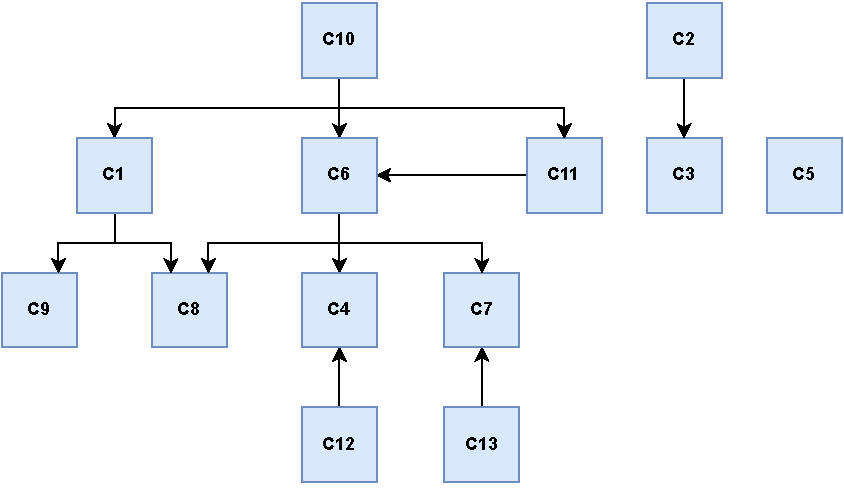
\includegraphics[width=0.87\linewidth]{figures/concept2concept.pdf}
    \caption[Dependencies between Conceptual Models]{Dependencies between
        Conceptual Models (Section~\ref{sec_conceptual})}
    \label{fig:conceptualdependencies}
\end{figure}
\vspace*{\fill}

\vspace*{\fill}
\begin{figure}[tbh]
    \centering
    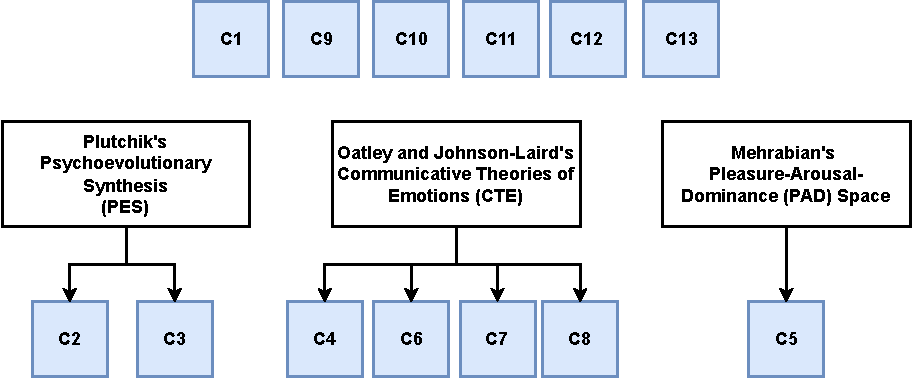
\includegraphics[width=\linewidth]{figures/theories2concept.pdf}
    \caption[Conceptual Model Dependencies on Affective
    Theories/Models]{Conceptual Model Dependencies on Affective Theories/Models
    (Section~\ref{sec_conceptual})}
    \label{fig:theories2conceptual}
\end{figure}
\vspace*{\fill}

\begin{figure}[tbh]
    \centering
    \includegraphics[height=0.96\textheight]{figures/assumptions2All.pdf}
    \caption[Dependencies on Assumptions]{Dependencies on Assumptions (Orange)
    (Section~\ref{sec_assumptions})}
    \label{fig:A2All}
\end{figure}

\begin{landscape}
    \begin{figure}[tbh]
        \centering
        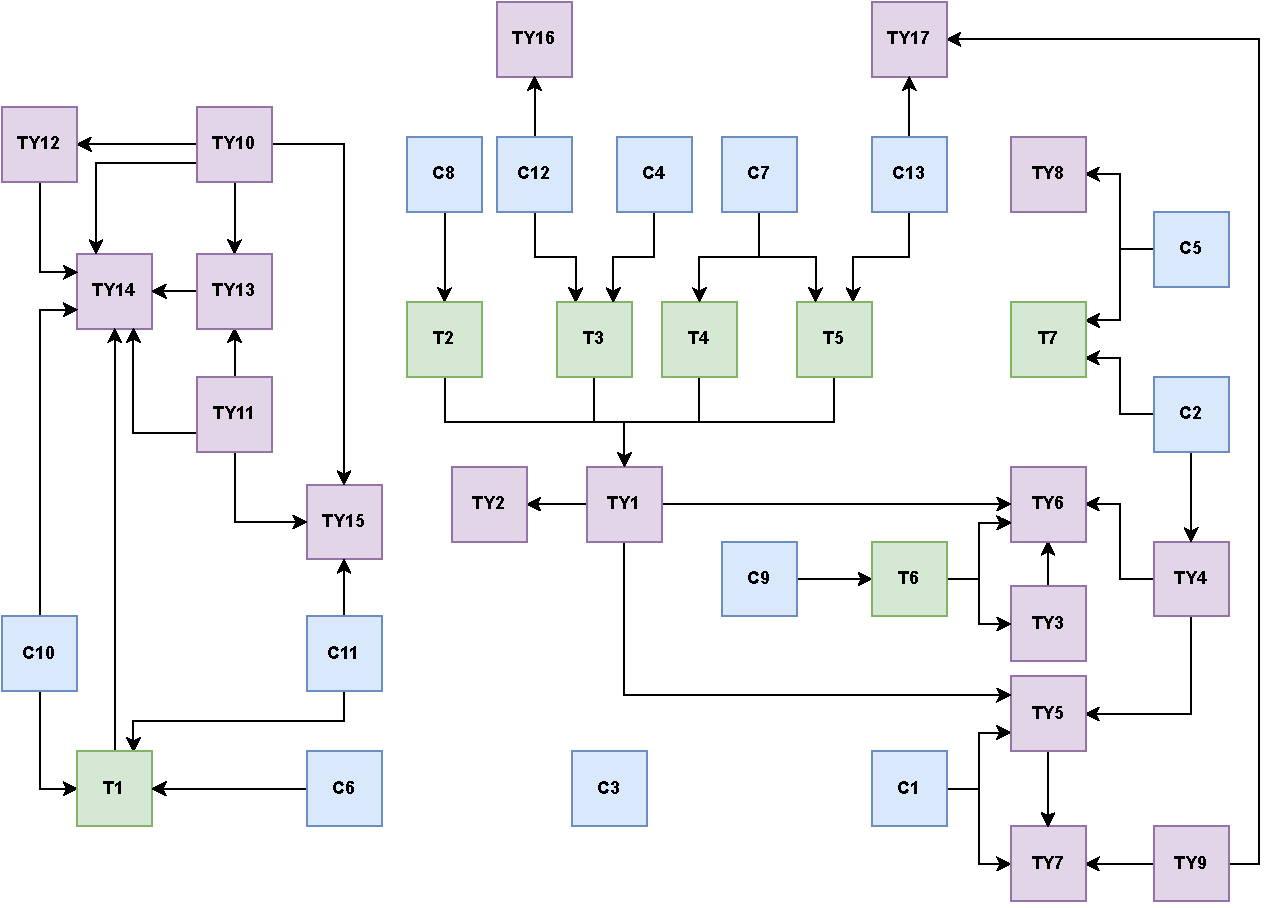
\includegraphics[width=\linewidth]{figures/concept2types_revised.pdf}
        \caption[Traceability between Theoretical Models and Data Types, and
        their dependencies on Conceptual Models]{Traceability between
        Theoretical Models (Green) and Data Types (Purple), and their
        dependencies on Conceptual Models (Blue)
        (Sections~\ref{sec_theoretical}, \ref{sec_typedefs},
        and~\ref{sec_conceptual})}
        \label{fig:C2TY}
    \end{figure}
\end{landscape}

\begin{landscape}
    \begin{figure}[tbh]
        \centering
        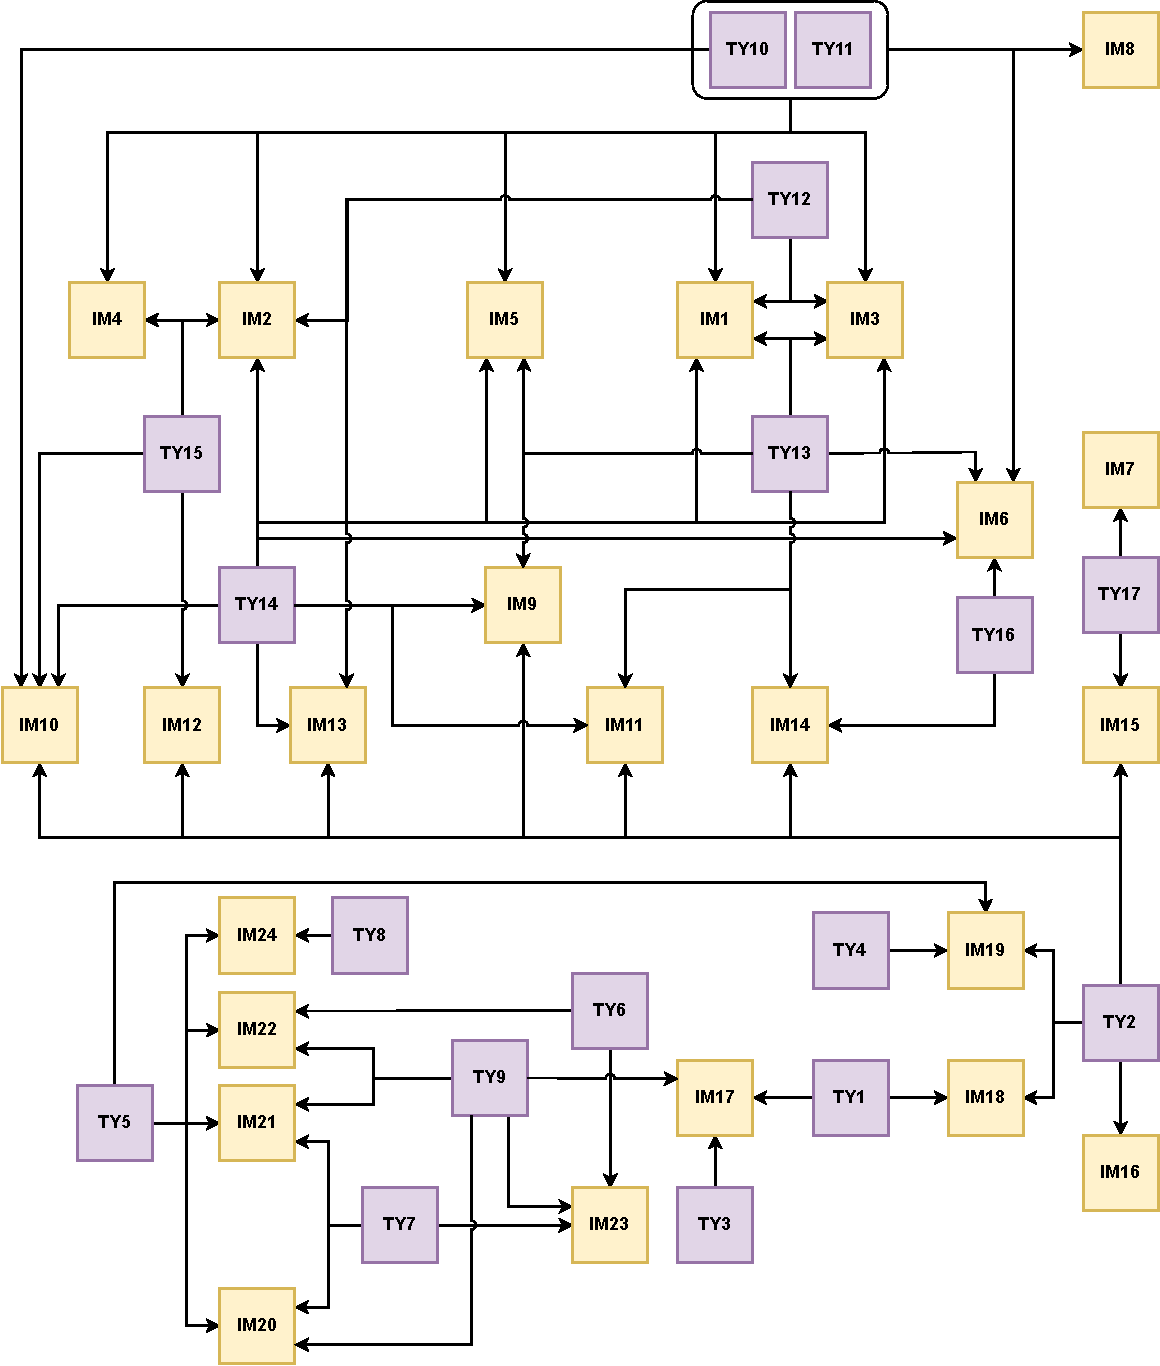
\includegraphics[width=0.88\linewidth]{figures/types2instance.pdf}
        \caption[Instance Models and their Dependencies on Theoretical Models
        and Data Types]{Instance Models (Yellow) and their Dependencies on
        Theoretical Models (Green) and Data Types (Purple)
        (Sections~\ref{sec_theoretical}, \ref{sec_typedefs},
        and~\ref{sec_instance})}
        \label{fig:T-TY2IM}
    \end{figure}
\end{landscape}

\vspace*{\fill}
\begin{figure}[tbh]
    \centering
    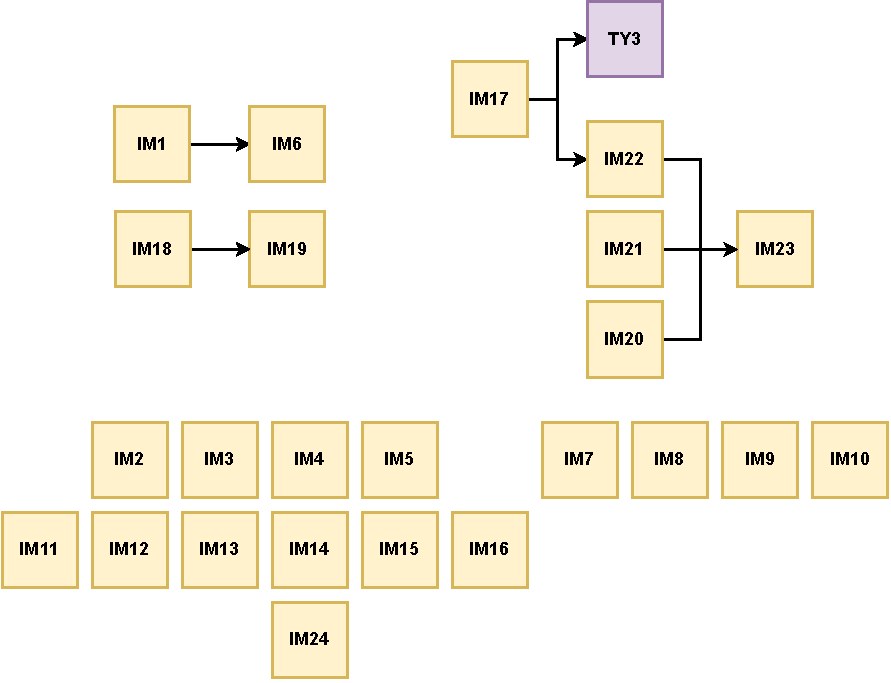
\includegraphics[width=0.5\linewidth]{figures/instance2instance.pdf}
    \caption[Dependencies between Instance Models]{Dependencies between
        Instance Models (Section~\ref{sec_instance})}
    \label{fig:IM}
\end{figure}
\vspace*{\fill}

\begin{figure}[tbh]
    \centering
    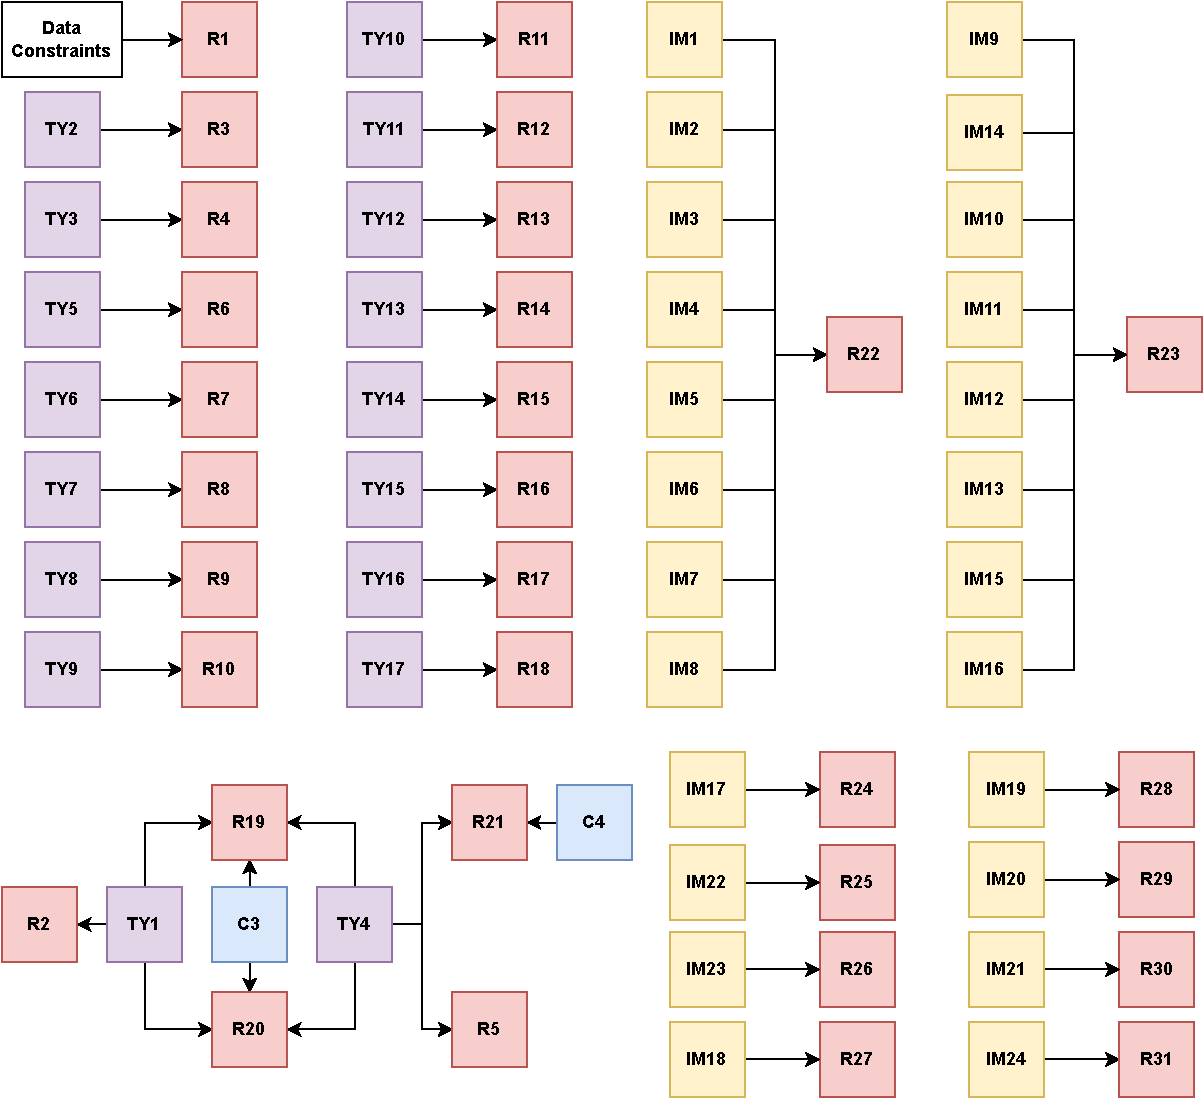
\includegraphics[width=\linewidth]{figures/reqs2All.pdf}
    \caption[Functional Requirements and their Dependencies on Conceptual
    Models, Data Types, Instance Models, and Data Constraints]{Functional
    Requirements (Red) and
    their Dependencies on Conceptual Models (Blue), Data Types (Purple),
    Instance Models (Yellow), and Data Constraints
    (Sections~\ref{sec_conceptual}, \ref{sec_typedefs}, \ref{sec_instance},
    \ref{sec_DataConstraints}, and \ref{sec_functionalreqs})}
    \label{fig:M2R}
\end{figure}

    \clearpage

    \bibliographystyle {ACM-Reference-Format}
    \bibliography{../../../refs/references_test,
    ../../../refs/references_gamedesign}

    \setcounter{pages}{\totalpages}

\end{document}